\section{问题重述}
\subsection{问题背景}
热风干燥通过烘房与药材之间的热量交换促进水分排出，是药材加工中的重要环节。作业通常经历升温预热和持续干燥两个阶段，温湿环境的设置及持续时间会影响脱水效率、能源消耗与成品状态。因此，需要掌握药材内部温度和水分的演化规律，为干燥进程控制和结束时间的判断提供依据。

药材内部的传热与水分迁移并不同步，表面和中心可能处于不同的干燥状态。随着水分减少，材料物性和外形尺寸也会变化，增加了过程预测的难度。依靠多次试验比较工况需要较多时间和成本，结合环境记录及材料参数建立数学模型，有助于分析局部温湿变化与整体干燥程度之间的关系。

\subsection{问题提出}
研究对象为一根初始长度0.25 m、半径0.02 m的圆柱形药材，初始温度为28\tempunit，干基含水率为2.55\cunit。附件1提供烘房环境随时间的记录，附件2给出药材半径的变化，各问所需热物性和扩散系数由相应附录给定。根据这些已知条件，需要完成以下四项任务。

\textbf{问题一：}采用附录2的参数，描述预热阶段药材内部温度与含水率的变化。计算前30 min的径向分布，在指定时刻和位置列示结果，并以1 s的时间间隔、0.1 cm的径向间隔保存完整数据。

\textbf{问题二：}统一采用附录3中随状态变化的物性关系，建立覆盖整个烘干过程的温湿变化模型。给出前3 h内每隔0.5 h、径向每隔0.5 cm的温度与含水率，同时按1 s和0.1 cm的间隔记录该时段的完整结果。

\textbf{问题三：}在问题二的条件下，以药材所有位置的含水率均小于0.15\cunit 为要求，确定所需烘干时间。每隔6 h展示径向间隔0.5 cm的含水率，补充结束时刻的分布，并按60 s和0.1 cm的间隔保存干燥历程。

\textbf{问题四：}考虑药材失水后的尺寸变化，结合附件2的半径记录和附录4的物性关系，重新预测达到相同含水率限值所需的时间。按问题三的时空间隔给出含水率结果，并记录实际表面状态，区分药材内部测点与收缩后已处于药材外的位置。

四问结果均保留四位小数，详细数据依照附件3的模板分别写入\texttt{result1.xlsx}--\texttt{result4.xlsx}。正文表1至表6汇列各问要求的代表性时空位置结果。

\newpage
\section{模型假设}
\begin{enumerate}[label=\arabic*、,ref=\arabic*,leftmargin=2em,labelsep=0pt,itemsep=0.5em,topsep=0.3em]
\item\label{assumption:radial} \textbf{只考虑径向传热传质：}忽略周向差异和轴向端部效应，认为同一半径处温度与含水率相同。
\item\label{assumption:continuum} \textbf{将药材视为连续有效介质：}不区分孔隙、液态水和水汽等微观迁移形式，其综合影响统一计入有效物性。
\item\label{assumption:equilibrium} \textbf{将环境水分浓度视为药材表面水分变化的平衡终点：}以药材表面含水率与环境水分浓度之差作为传质驱动力。
\item\label{assumption:sensible-heat} \textbf{忽略其他次要热效应：}不考虑辐射、化学反应、蒸发潜热及收缩做功，仅考虑热传导和表面对流换热。
\item\label{assumption:shrinkage} \textbf{假设药材发生同源径向收缩：}问题四中药材保持圆柱形且长度不变，各物质点随半径同比例收缩。
\end{enumerate}

\section{问题分析}
四问的区别在于模型逐步增加了什么：问题一计算预热分布，问题二引入温湿耦合，问题三增加达标判据，问题四再考虑半径收缩。图\ref{fig:framework}给出各问之间的衔接关系，具体方程与算法放在对应问题中说明。

\begin{figure}[!htbp]
\centering
% 图1：与图5统一浅灰填充、宋体字号、圆角和箭头样式。
% 虚线表示各问模型的逐步扩展，不表示初始状态的传递。
\begin{tikzpicture}[
  box/.style={draw,rounded corners=2pt,fill=black!3,align=center,
    minimum height=1.05cm,inner sep=5pt,font=\small},
  task/.style={box,text width=3.05cm,minimum height=2.55cm},
  flow/.style={-{Stealth[length=2mm]},semithick},
  connector/.style={semithick},
  every node/.append style={font=\small}
]
  \node[box,text width=8.0cm] (input) at (0,0)
    {烘干条件与药材参数\\整理温湿记录、物性关系和半径变化};
  \node[box,text width=14.45cm] (model) at (0,-1.5)
    {建立径向传热传质模型\\结合中心对称与表面交换条件，用有限体积法求解};

  \node[task] (p1) at (-5.7,-3.95)
    {问题一\\[4pt]分析预热过程\\采用常热物性\\
     分别求解温湿场\\给出前30分钟分布};
  \node[task] (p2) at (-1.9,-3.95)
    {问题二\\[4pt]分析全程温湿变化\\计入物性变化\\
     联立求解温湿场\\给出前3小时分布};
  \node[task] (p3) at (1.9,-3.95)
    {问题三\\[4pt]确定烘干时间\\沿用问题二模型\\
     检查最大含水率\\求得整体达标时刻};
  \node[task] (p4) at (5.7,-3.95)
    {问题四\\[4pt]考虑药材收缩\\由记录确定半径\\
     转至物质坐标求解\\计算所需烘干时间};

  \node[box,text width=14.45cm] (check) at (0,-6.4)
    {检验结果并分析误差\\与半解析解对照，检查网格与步长影响，考察参数变化};

  \draw[flow] (input.south) -- (model.north);
  \draw[connector] (model.south) -- (0,-2.32);
  \draw[connector] (-5.7,-2.32) -- (5.7,-2.32);
  \foreach \x/\p in {-5.7/p1,-1.9/p2,1.9/p3,5.7/p4} {
    \draw[flow] (\x,-2.32) -- (\p.north);
    \draw[connector] (\p.south) -- (\x,-5.6);
  }
  \draw[connector] (-5.7,-5.6) -- (5.7,-5.6);
  \draw[flow] (0,-5.6) -- (check.north);
  \draw[flow,dashed] (p1.east) -- (p2.west);
  \draw[flow,dashed] (p2.east) -- (p3.west);
  \draw[flow,dashed] (p3.east) -- (p4.west);
\end{tikzpicture}

\caption{药材烘干问题的总体求解框架}
\label{fig:framework}
\end{figure}

\subsection{问题一分析}
问题一需要研究预热阶段药材内部温度与含水率的径向分布。由于药材内部存在不可忽略的传热传质阻力，不能将其视为均匀状态，因此需分别建立径向热传导和水分扩散模型。结合题目给定的常热物性参数，采用有限体积法对空间进行离散，并逐步计算不同时间、不同位置的温度和含水率。

\subsection{问题二分析}
问题二进一步考虑物性随状态变化，使温度影响水分扩散、水分变化又反过来影响传热，原有两个独立过程转变为热质耦合过程。因此在问题一模型基础上，引入变物性关系，并在每个时间步同步更新温度、含水率及相关物性，研究前3 h内两场的共同演化。

\subsection{问题三分析}
问题三需要确定药材整体达到含水率要求的时间，其关键在于不能仅以表面或平均含水率作为判据，而应保证所有位置均低于$0.15\cunit$。因此沿用问题二的热质耦合模型继续计算，并实时跟踪全域最大含水率，通过阈值穿越确定最终烘干时刻。

\subsection{问题四分析}
问题四进一步考虑药材失水引起的尺寸收缩，使计算区域由固定区域转变为随时间变化的移动区域。为便于计算，可将变化的物理区域映射到固定坐标区间，并结合附录4的物性关系重新描述传热传质过程，最终仍以全域含水率是否达标作为烘干终点判据。

\section{符号说明}
\begingroup
\setlength{\LTpre}{6pt}
\setlength{\LTpost}{6pt}
\begin{longtable*}{@{}>{\centering\arraybackslash}m{0.16\textwidth}>{\centering\arraybackslash}m{\dimexpr0.56\textwidth-4\tabcolsep\relax}>{\centering\arraybackslash}m{0.28\textwidth}@{}}
\toprule
符号 & 含义 & 单位\\\midrule
\endfirsthead
\toprule
符号 & 含义 & 单位\\\midrule
\endhead
\bottomrule
\endfoot
$t$ & 时间 & s\\
$r$ & 距圆柱轴线的径向距离 & m\\
$R_0$ & 药材初始半径 & m\\
$R(t)$ & 药材当前半径 & m\\
$L$ & 药材长度 & m\\
$T$ & 药材温度 & $^{\circ}$C\\
$T_a$ & 烘房环境温度 & $^{\circ}$C\\
$T_K$ & 药材绝对温度 & K\\
$C$ & 药材干基含水率 & kg/kg\\
$C_a$ & 表面传质的有效平衡含水率 & kg/kg\\
$C_*$ & 干燥达标含水率限值 & kg/kg\\
$\rho$ & 药材有效密度 & kg/m$^3$\\
$c_p$ & 比热容 & J/(kg K)\\
$k$ & 热传导系数 & W/(m K)\\
$D$ & 有效水分扩散系数 & m$^2$/s\\
$h$ & 表面对流换热系数 & W/(m$^2$ K)\\
$h_m$ & 表面对流传质系数 & m/s\\
$\xi$ & 随骨架运动的归一化径向坐标 & 1\\
$V_i$ & 物理坐标下的径向控制体积分权重 & m$^2$\\
$G_{i+1/2}$ & 控制面导通系数 & \shortstack{W/(m K)（传热）\\m$^2$/s（传质）}\\
$\theta$ & 时间格式权重 & 1\\
$\Delta t$ & 计算时间步长 & s\\
$t_*$ & 临界达标时刻 & s\\
$\overline C$ & 截面加权平均含水率 & kg/kg\\
\end{longtable*}
\addtocounter{table}{-1}% 无标题符号表不占用题目规定的结果表编号。
\endgroup
热方程中的温差可用摄氏温度计算；所有指数式中的温度严格取$T_K=T+273.15$。输入半径由cm换算为m，输出时再换回cm。为避免混淆，场量的偏导数均以分式书写，$s$、$a$等物理标记与$i$等离散索引保留为下标。

\section{问题一模型的建立与求解}
\label{sec:p1}
% 本文件包含第五节的5.1；模型求解与结果分析分别见同目录下的对应文件。
\subsection{模型建立}
\label{sec:p1-model}

问题一要求描述预热阶段药材内部的温度和含水率分布。依据前述假设，首先利用几何尺度确定空间描述的维度，再比较内部传递与表面交换的相对强弱，判断是否需要保留内部梯度；在此基础上，由能量守恒和水质量连续性建立控制方程，并结合环境记录确定初边值条件。

\subsubsection{径向分布模型的选择}

药材长度$L=0.25\ \mathrm{m}$、半径$R_0=0.02\ \mathrm{m}$，长径比
$L/(2R_0)=6.25$，两端面积占总表面积的比例为$R_0/(L+R_0)=7.41\%$。
依据假设\ref{assumption:radial}，忽略轴向影响，只考虑径向传热传质，以远离端部的中部截面为代表，建立径向模型$T(r,t)$、$C(r,t)$。

毕渥数用于比较内部传递阻力与表面交换阻力\cite{heat}。
题给$h=25\ \mathrm{W/(m^2 K)}$、$k=0.36\ \mathrm{W/(m K)}$、
$h_m=8\times10^{-7}\ \mathrm{m/s}$，水分扩散系数为
\begin{equation}
  D(C)=7\times10^{-9}\exp\!\left(-\frac{0.89}{C}\right)\ \mathrm{m^2/s},
  \label{eq:p1-diffusivity}
\end{equation}
初始含水率$C_0=2.55\cunit$对应$D(C_0)=4.9377\times10^{-9}\ \mathrm{m^2/s}$。
以半径为特征长度，热、质毕渥数分别为
\begin{equation}
  Bi_T=\frac{hR_0}{k}=1.3889,\qquad
  Bi_C(C_0)=\frac{h_mR_0}{D(C_0)}=3.2404.
  \label{eq:p1-biot}
\end{equation}
两者均达到单位量级；即使用圆柱体积与侧面积之比$L_c=R_0/2$作为集总判据的特征长度，
热毕渥数仍为$0.6944>0.1$。失水还会减小$D(C)$、增大传质毕渥数，故须保留内部径向梯度。

\subsubsection{由守恒关系建立热量与水分传递方程}

设$\rho_d$为单位药材体积中的干物质质量，水质量密度为$w=\rho_d C$。
固定、静止且均匀的干骨架近似下，$\rho_d$为常数；它与热容量中的有效密度$\rho$含义不同。
取径向向外为水质量通量$j_w$的正方向，由圆柱壳层的水质量收支及菲克定律\cite{fick}得
\begin{equation}
\begin{aligned}
  \frac{\partial w}{\partial t}
    +\frac{1}{r}\frac{\partial}{\partial r}(rj_w)&=0,\\
  j_w=-D(C)\frac{\partial w}{\partial r}
    &=-\rho_dD(C)\frac{\partial C}{\partial r}.
\end{aligned}
  \label{eq:p1-water-continuity}
\end{equation}
式\eqref{eq:p1-water-continuity}中第一式为水质量连续性方程。
将$w=\rho_d C$及通量关系代入该式，约去$\rho_d$，得到
\begin{equation}
  \boxed{\frac{\partial C}{\partial t}
  =\frac{1}{r}\frac{\partial}{\partial r}
    \left[rD(C)\frac{\partial C}{\partial r}\right].}
  \label{eq:p1-mass}
\end{equation}
由于$D(C)$随局部含水率变化，须将其保留在空间导数内部。

按照假设\ref{assumption:sensible-heat}，仅计显热储存和导热。
以$q_T$表示径向向外的热流密度，能量守恒与傅里叶定律为\cite{heat}
\begin{equation}
  \rho c_p\frac{\partial T}{\partial t}
  +\frac{1}{r}\frac{\partial}{\partial r}(rq_T)=0,\qquad
  q_T=-k\frac{\partial T}{\partial r}.
  \label{eq:p1-energy-fourier}
\end{equation}
代入常热物性$\rho=820\ \mathrm{kg/m^3}$、$c_p=2600\ \mathrm{J/(kg\,K)}$、
$k=0.36\ \mathrm{W/(m\,K)}$及热流关系，得
\begin{equation}
  \boxed{\rho c_p\frac{\partial T}{\partial t}
  =\frac{k}{r}\frac{\partial}{\partial r}
    \left(r\frac{\partial T}{\partial r}\right).}
  \label{eq:p1-heat}
\end{equation}
两场的求解区域均为$0<r<R_0$、$0<t\le1800\ \mathrm{s}$。

\subsubsection{初始条件与时变边界条件的确立}

药材初始温湿状态均匀，取
\begin{equation}
  T(r,0)=28\tempunit,\qquad
  C(r,0)=2.55\cunit,\qquad 0\le r\le R_0.
  \label{eq:p1-initial}
\end{equation}
中心满足轴对称条件：
\begin{equation}
  \left.\frac{\partial T}{\partial r}\right|_{r=0}=0,\qquad
  \left.\frac{\partial C}{\partial r}\right|_{r=0}=0.
  \label{eq:p1-center}
\end{equation}

记表面值$T_s=T(R_0,t)$、$C_s=C(R_0,t)$。
按假设\ref{assumption:equilibrium}，将环境水分浓度视为有效平衡含水率$C_a(t)$，
表面水质量交换通量为$\rho_dh_m[C_s-C_a(t)]$。
令内部通量与表面对流交换相等，并在传质关系中约去$\rho_d$，得到第三类边界条件
\begin{align}
  -k\left.\frac{\partial T}{\partial r}\right|_{r=R_0}
    &=h[T_s-T_a(t)],\label{eq:p1-boundary-heat}\\
  -D(C_s)\left.\frac{\partial C}{\partial r}\right|_{r=R_0}
    &=h_m[C_s-C_a(t)].\label{eq:p1-boundary-mass}
\end{align}
表面值由环境交换与内部传递共同确定，仍是模型的未知量。
图\ref{fig:p1-schematic}概括了药材内部的径向传递过程及表面与烘房之间的热质交换关系。

\pfig{图2.png}{0.82}{问题一圆柱药材径向传热传质模型示意图}{fig:p1-schematic}

为给上述边界条件提供任意时刻的环境值，需要进一步处理附件1的离散记录。
附件1每隔$60\ \mathrm{s}$记录环境状态。为获取中间时刻信息并减小误差，
记记录时刻及对应环境值为$t_j$、$y_{a,j}$，对$y_a\in\{T_a,C_a\}$作分段线性插值\cite{num}：
\begin{equation}
  y_a(t)=y_{a,j}
  +\frac{t-t_j}{t_{j+1}-t_j}(y_{a,j+1}-y_{a,j}),
  \qquad t_j\le t\le t_{j+1}.
  \label{eq:p1-environment}
\end{equation}
如图\ref{fig:p1-environment}所示，前$4\ \mathrm{h}$采用记录插值，
此后恒定延拓为$T_a=50\tempunit$、$C_a=0.05\cunit$。
本问的$0$--$1800\ \mathrm{s}$均位于记录区间内，直接以插值结果驱动表面边界。

\pfig{图3.pdf}{0.88}{烘房环境记录的分段线性插值及恒定延拓}{fig:p1-environment}

式\eqref{eq:p1-mass}、式\eqref{eq:p1-heat}及上述初边值条件构成完整模型。
本问热方程及其边界不含$C$，水分方程及其边界不含$T$，两场相互独立，可分别求解。

% 5.2：参考先前独立求解稿，压缩为离散边界处理、线性系统及题目规定结果。
% 表1、表2沿用结果/p1_论文表格.md；本次写作未重算生产解。
\subsection{模型求解}
\label{sec:p1-solution}

上节建立的温度方程与水分方程具有相同的扩散结构。以$u$表示待求场量，
两个初边值问题的一般形式为
\begin{equation*}
\begin{gathered}
  a\frac{\partial u}{\partial t}
    =\frac{1}{r}\frac{\partial}{\partial r}
      \left(r\Gamma\frac{\partial u}{\partial r}\right),
    \qquad 0<r<R_0,\quad 0<t\le1800\ \mathrm{s},\\
  u(r,0)=u_0,\qquad
  \left.\frac{\partial u}{\partial r}\right|_{r=0}=0,\qquad
  -\left.\Gamma\frac{\partial u}{\partial r}\right|_{r=R_0}
    =\beta[u(R_0,t)-u_a(t)].
\end{gathered}
\end{equation*}
其中，温度场取$u=T$、$(a,\Gamma,\beta,u_a)=(\rho c_p,k,h,T_a)$、
$u_0=28\tempunit$；水分场取$u=C$、$(a,\Gamma,\beta,u_a)=(1,D(C),h_m,C_a)$、
$u_0=2.55\cunit$。式\eqref{eq:p1-environment}已将离散记录转化为任意时刻可取值的环境函数。
有限体积法以控制体上的积分守恒关系为基础，能够在离散层面较好地体现热量与水分的局部及整体守恒\cite{nht}。
因此，本文采用有限体积法进行空间离散，将上述偏微分方程化为节点值的常微分方程组，
再通过隐式时间推进形成可求解的线性系统。

\subsubsection{将边界条件纳入空间离散}

取节点$0=r_0<r_1<\cdots<r_N=R_0$，令$u_i(t)\approx u(r_i,t)$。
以相邻节点中点$r_{i+1/2}=(r_i+r_{i+1})/2$为内部控制面，并令
$r_{-1/2}=0$、$r_{N+1/2}=R_0$，则第$i$个控制体对应区间
$[r_{i-1/2},r_{i+1/2}]$，中心和表面处的控制体由边界截断。
按圆柱体积元$2\pi Lr\,\dd r$在该控制体上对一般方程积分，
并约去公共因子$2\pi L$，得到
\begin{equation*}
  \int_{r_{i-1/2}}^{r_{i+1/2}}
    a\frac{\partial u}{\partial t}\,r\,\dd r
  =\left.r\Gamma\frac{\partial u}{\partial r}\right|_{r_{i+1/2}}
   -\left.r\Gamma\frac{\partial u}{\partial r}\right|_{r_{i-1/2}}.
\end{equation*}
这一步仍是精确的控制体收支关系：左端为储存率，右端为通过两个控制面的净输入。
空间散度已化为面值之差，接下来只需用离散节点值近似储存项和面通量。
为此定义
\begin{equation}
\begin{gathered}
  V_i=\frac{r_{i+1/2}^{2}-r_{i-1/2}^{2}}{2},\qquad
  G_{i+1/2}=\frac{r_{i+1/2}\Gamma_{i+1/2}}{r_{i+1}-r_i},\\
  \Gamma_{i+1/2}=\frac{\Gamma_i+\Gamma_{i+1}}{2},\qquad B=R_0\beta.
\end{gathered}
\label{eq:p1-fvm-coefficients}
\end{equation}
其中$V_i=\int_{r_{i-1/2}}^{r_{i+1/2}}r\,\dd r$为控制体积权重，
$G_{i+1/2}$合并了控制面半径、面物性及节点间距。
用节点$i$处的变化率代表控制体内的储存率，左端近似为
\begin{equation*}
  \int_{r_{i-1/2}}^{r_{i+1/2}}
    a\frac{\partial u}{\partial t}\,r\,\dd r
  \approx aV_i\frac{\dd u_i}{\dd t}.
\end{equation*}
对内部控制面，用跨越该面的相邻节点差商近似梯度，便有
\begin{equation*}
  \left.r\Gamma\frac{\partial u}{\partial r}\right|_{r_{i+1/2}}
  \approx
  r_{i+1/2}\Gamma_{i+1/2}\frac{u_{i+1}-u_i}{r_{i+1}-r_i}
  =G_{i+1/2}(u_{i+1}-u_i),\qquad 0\le i<N.
\end{equation*}
内侧控制面的对应项为$G_{i-1/2}(u_i-u_{i-1})$。
将外、内两个面值相减，内部控制体的净输入即化为
$G_{i-1/2}(u_{i-1}-u_i)+G_{i+1/2}(u_{i+1}-u_i)$。

两个边界面按已建立的边界条件处理。中心处的对称条件给出零通量，且该面的面积为零；
表面处则直接将第三类边界代入积分式，得到
\begin{equation*}
  \left.r\Gamma\frac{\partial u}{\partial r}\right|_{r=R_0}
  =R_0\beta[u_a(t)-u_N]
  =B[u_a(t)-u_N].
\end{equation*}
该项表示环境向表面控制体的净输入，环境值$u_a(t)$已知，表面值$u_N(t)$仍需与内部节点一同求解。
将储存项、内部面通量及边界通量合并，对全部控制体统一写为
\begin{equation}
  aV_i\frac{\dd u_i}{\dd t}
  =G_{i-1/2}(u_{i-1}-u_i)+G_{i+1/2}(u_{i+1}-u_i)
    +\delta_{iN}B[u_a(t)-u_N].
  \label{eq:p1-fvm}
\end{equation}
这里$\delta_{iN}$仅在表面节点$i=N$时为1，不存在的边界邻接项取零。
由此，原偏微分方程中的空间导数被相邻节点之间的交换项代替，仅保留各节点关于时间的导数。
表面通量由边界条件直接给出，无需引入虚拟节点，
式\eqref{eq:p1-fvm}明确了时变环境进入数值模型的位置。

\subsubsection{时间推进与线性方程组的形成}

令$t^n=n\Delta t$，在一次物性固定的计算中，将式\eqref{eq:p1-fvm}右端记为
$\mathcal L_i(\boldsymbol u;u_a)$，采用
\begin{equation}
  \frac{aV_i}{\Delta t}(u_i^{n+1}-u_i^n)
  =(1-\theta)\mathcal L_i(\boldsymbol u^n;u_a^n)
    +\theta\mathcal L_i(\boldsymbol u^{n+1};u_a^{n+1}),
  \label{eq:p1-time}
\end{equation}
其中$u_a^n=u_a(t^n)$、$u_a^{n+1}=u_a(t^{n+1})$均由插值式\eqref{eq:p1-environment}取得。
常规步取$\theta=1/2$，对温度方程即为Crank--Nicolson格式\cite{cn}。
为衰减初始均匀场与表面立即失水之间的失配所激发的快速分量，前两步取$\theta=1$作隐式阻尼启动。

记$m_i=aV_i/\Delta t$、$S_i=G_{i-1/2}+G_{i+1/2}+\delta_{iN}B$，
并令$d_i=m_i+\theta S_i$，不存在的边界邻接项仍取零。
将本次待求的新层节点值记为$x_i$，把式\eqref{eq:p1-time}中的未知项移至左端，
按从中心到表面的节点顺序排列，得到三对角线性方程组
\begin{equation}
\setlength{\arraycolsep}{3pt}
\begin{pmatrix}
  d_0 & -\theta G_{1/2} & 0 & \cdots & 0\\
  -\theta G_{1/2} & d_1 & -\theta G_{3/2} & \ddots & \vdots\\
  0 & \ddots & \ddots & \ddots & 0\\
  \vdots & \ddots & -\theta G_{N-3/2} & d_{N-1} & -\theta G_{N-1/2}\\
  0 & \cdots & 0 & -\theta G_{N-1/2} & d_N
\end{pmatrix}
\begin{pmatrix}
  x_0\\x_1\\\vdots\\x_{N-1}\\x_N
\end{pmatrix}
=
\begin{pmatrix}
  b_0\\b_1\\\vdots\\b_{N-1}\\b_N
\end{pmatrix}.
\label{eq:p1-linear-system}
\end{equation}
系数矩阵除主对角线及其上下相邻两条副对角线外均为零，反映每个控制体仅与相邻控制体直接交换热量或水分，非相邻位置的影响通过逐层传递实现。
其中，中心处的主对角元为$d_0=m_0+\theta G_{1/2}$，
表面处为$d_N=m_N+\theta(G_{N-1/2}+B)$；
右端向量的各分量为
\begin{equation*}
  b_i=m_i u_i^n+(1-\theta)\mathcal L_i(\boldsymbol u^n;u_a^n)
       +\delta_{iN}\theta B u_a^{n+1},\qquad 0\le i\le N.
\end{equation*}
右端的旧层场、环境值和本轮固定的系数均已知，因此可直接求出本轮的全部节点值。
矩阵首行已纳入中心零通量条件；为明确时变环境的作用，将对应表面节点的最后一行展开为
\begin{equation}
\begin{aligned}
  &-\theta G_{N-1/2}x_{N-1}
    +[m_N+\theta(G_{N-1/2}+B)]x_N\\
  &\quad=[m_N-(1-\theta)(G_{N-1/2}+B)]u_N^n
    +(1-\theta)G_{N-1/2}u_{N-1}^n\\
  &\qquad\quad+B[(1-\theta)u_a^n+\theta u_a^{n+1}].
\end{aligned}
\label{eq:p1-surface-row}
\end{equation}
\begin{samepage}
\textbf{环境在步首、步末的已知值加权后进入右端，未知表面值的交换系数$\theta B$则加入主对角元。}
这使离散且随时间变化的边界数据在每一步都有明确的进入位置，并保持方程组的三对角结构。
\par\end{samepage}

温度场的$\Gamma=k$为常数，每步直接求得$\boldsymbol x=\boldsymbol T^{n+1}$。
水分场的扩散系数依赖未知含水率，采用Picard迭代：
从$\boldsymbol C^{n+1,(0)}=\boldsymbol C^n$开始，第$\ell$轮按中点状态计算节点物性
\begin{equation}
  \Gamma_i^{(\ell)}
  =D\!\left(\frac{C_i^n+C_i^{n+1,(\ell)}}{2}\right),
  \label{eq:p1-midpoint-picard}
\end{equation}
再依式\eqref{eq:p1-fvm-coefficients}计算面系数，并在新、旧两层通量中使用同一组固定的
$G^{(\ell)}$，由式\eqref{eq:p1-linear-system}求出
$\boldsymbol x=\boldsymbol C^{n+1,(\ell+1)}$。
对参与Picard迭代的场，以相邻两轮迭代的最大改变量作为停止判据，
温度与含水率的容差分别规定为
\begin{equation}
  \left\|\boldsymbol T^{n+1,(\ell+1)}
       -\boldsymbol T^{n+1,(\ell)}\right\|_\infty
       <10^{-6}\tempunit,\qquad
  \left\|\boldsymbol C^{n+1,(\ell+1)}
       -\boldsymbol C^{n+1,(\ell)}\right\|_\infty
       <10^{-6}\cunit.
  \label{eq:picard-tolerance}
\end{equation}
其中$\|\cdot\|_\infty$表示所有径向节点上绝对值的最大值。
本问温度场无需迭代，仅检验含水率条件，迭代上限为20次。
在$\theta=1/2$的常规步中，这一处理对应含水率中点状态上的非线性通量近似。
环境时变直接更新右端末分量，水分方程的矩阵则还会随迭代物性更新。

\subsubsection{数值实现与计算结果}

各轮矩阵严格对角占优，具有唯一解\cite{num}；在Python中调用SciPy的
\texttt{solve\_banded}求解式\eqref{eq:p1-linear-system}，单次运算量为$O(N)$。
为分辨初期表面失水，采用882节点网格，在外侧$0.5\ \mathrm{mm}$加密；
取$\Delta t=0.03125\ \mathrm{s}$推进至$1800\ \mathrm{s}$，环境插值折点均落在时间层上。

每隔$1\ \mathrm{s}$在$r=0,0.1,\ldots,2.0\ \mathrm{cm}$处提取两场结果，
以四位小数写入\texttt{result1.xlsx}；题定7个时刻、5个径向位置的结果见
表\ref{tab:p1T}、表\ref{tab:p1C}。

\begin{table}[!htbp]
  \centering
  \caption{30分钟内药材的温度（单位：$^{\circ}\mathrm{C}$）}
  \label{tab:p1T}
  \begin{tabularx}{\textwidth}{@{}YYYYYY@{}}
    \toprule
    \multirow{2}{*}{时间/$\mathrm{s}$}&\multicolumn{5}{c}{到药材中心的距离/$\mathrm{cm}$}\\
    \cmidrule(lr){2-6}
    &0&0.5&1&1.5&2\\
    \midrule
    100  &28.0001&28.0003&28.0040&28.0327&28.1801\\
    300  &28.0408&28.0635&28.1514&28.3681&28.8489\\
    600  &28.4533&28.5360&28.8039&29.3159&30.1652\\
    900  &29.3243&29.4583&29.8755&30.6161&31.7304\\
    1200 &30.5427&30.7098&31.2223&32.1126&33.4276\\
    1500 &31.9957&32.1867&32.7660&33.7463&35.1203\\
    1800 &33.5753&33.7720&34.3642&35.3621&36.7856\\
    \bottomrule
  \end{tabularx}
\end{table}

\begin{table}[!htbp]
  \centering
  \caption{30分钟内药材的水分浓度（单位：$\mathrm{kg/kg}$）}
  \label{tab:p1C}
  \begin{tabularx}{\textwidth}{@{}YYYYYY@{}}
    \toprule
    \multirow{2}{*}{时间/$\mathrm{s}$}&\multicolumn{5}{c}{到药材中心的距离/$\mathrm{cm}$}\\
    \cmidrule(lr){2-6}
    &0&0.5&1&1.5&2\\
    \midrule
    100  &2.5500&2.5500&2.5500&2.5500&2.2471\\
    300  &2.5500&2.5500&2.5500&2.5492&2.0509\\
    600  &2.5500&2.5500&2.5500&2.5353&1.8770\\
    900  &2.5500&2.5500&2.5497&2.5045&1.7547\\
    1200 &2.5500&2.5500&2.5482&2.4646&1.6586\\
    1500 &2.5500&2.5499&2.5445&2.4206&1.5787\\
    1800 &2.5500&2.5497&2.5383&2.3755&1.5102\\
    \bottomrule
  \end{tabularx}
\end{table}

% 5.3：依据表1、表2与同源的已保存数值场分析结果；图3、图4均使用用户提供的PNG。
\subsection{结果分析}
\label{sec:p1-analysis}

\subsubsection{温度分布与升温滞后}

图\ref{fig:p1-temperature}显示，高温区域由表面向内部扩展，中心升温滞后。
$1800\ \mathrm{s}$时，中心与表面温度分别为$33.5753\tempunit$、$36.7856\tempunit$，
径向温差为$3.2103\tempunit$，表面仍比环境低约$4.73\tempunit$。

\begin{figure}[!htbp]
\centering
% 保持原图3的0.98\textwidth宽度及264.543625/636.93875高宽比。
% 裁去白边并压缩(a)主图与色条的间距，扩展主图裁剪以保留横排刻度及纵轴文字。
% trim按源PNG的300 dpi换算；各部分仅指定高度，保持原始比例和图组占位。
\setlength{\unitlength}{0.98\textwidth}
\begin{picture}(1,0.41533605)
  % A
  \put(0.015715190,0.004523636){\makebox(0,0)[lb]{%
    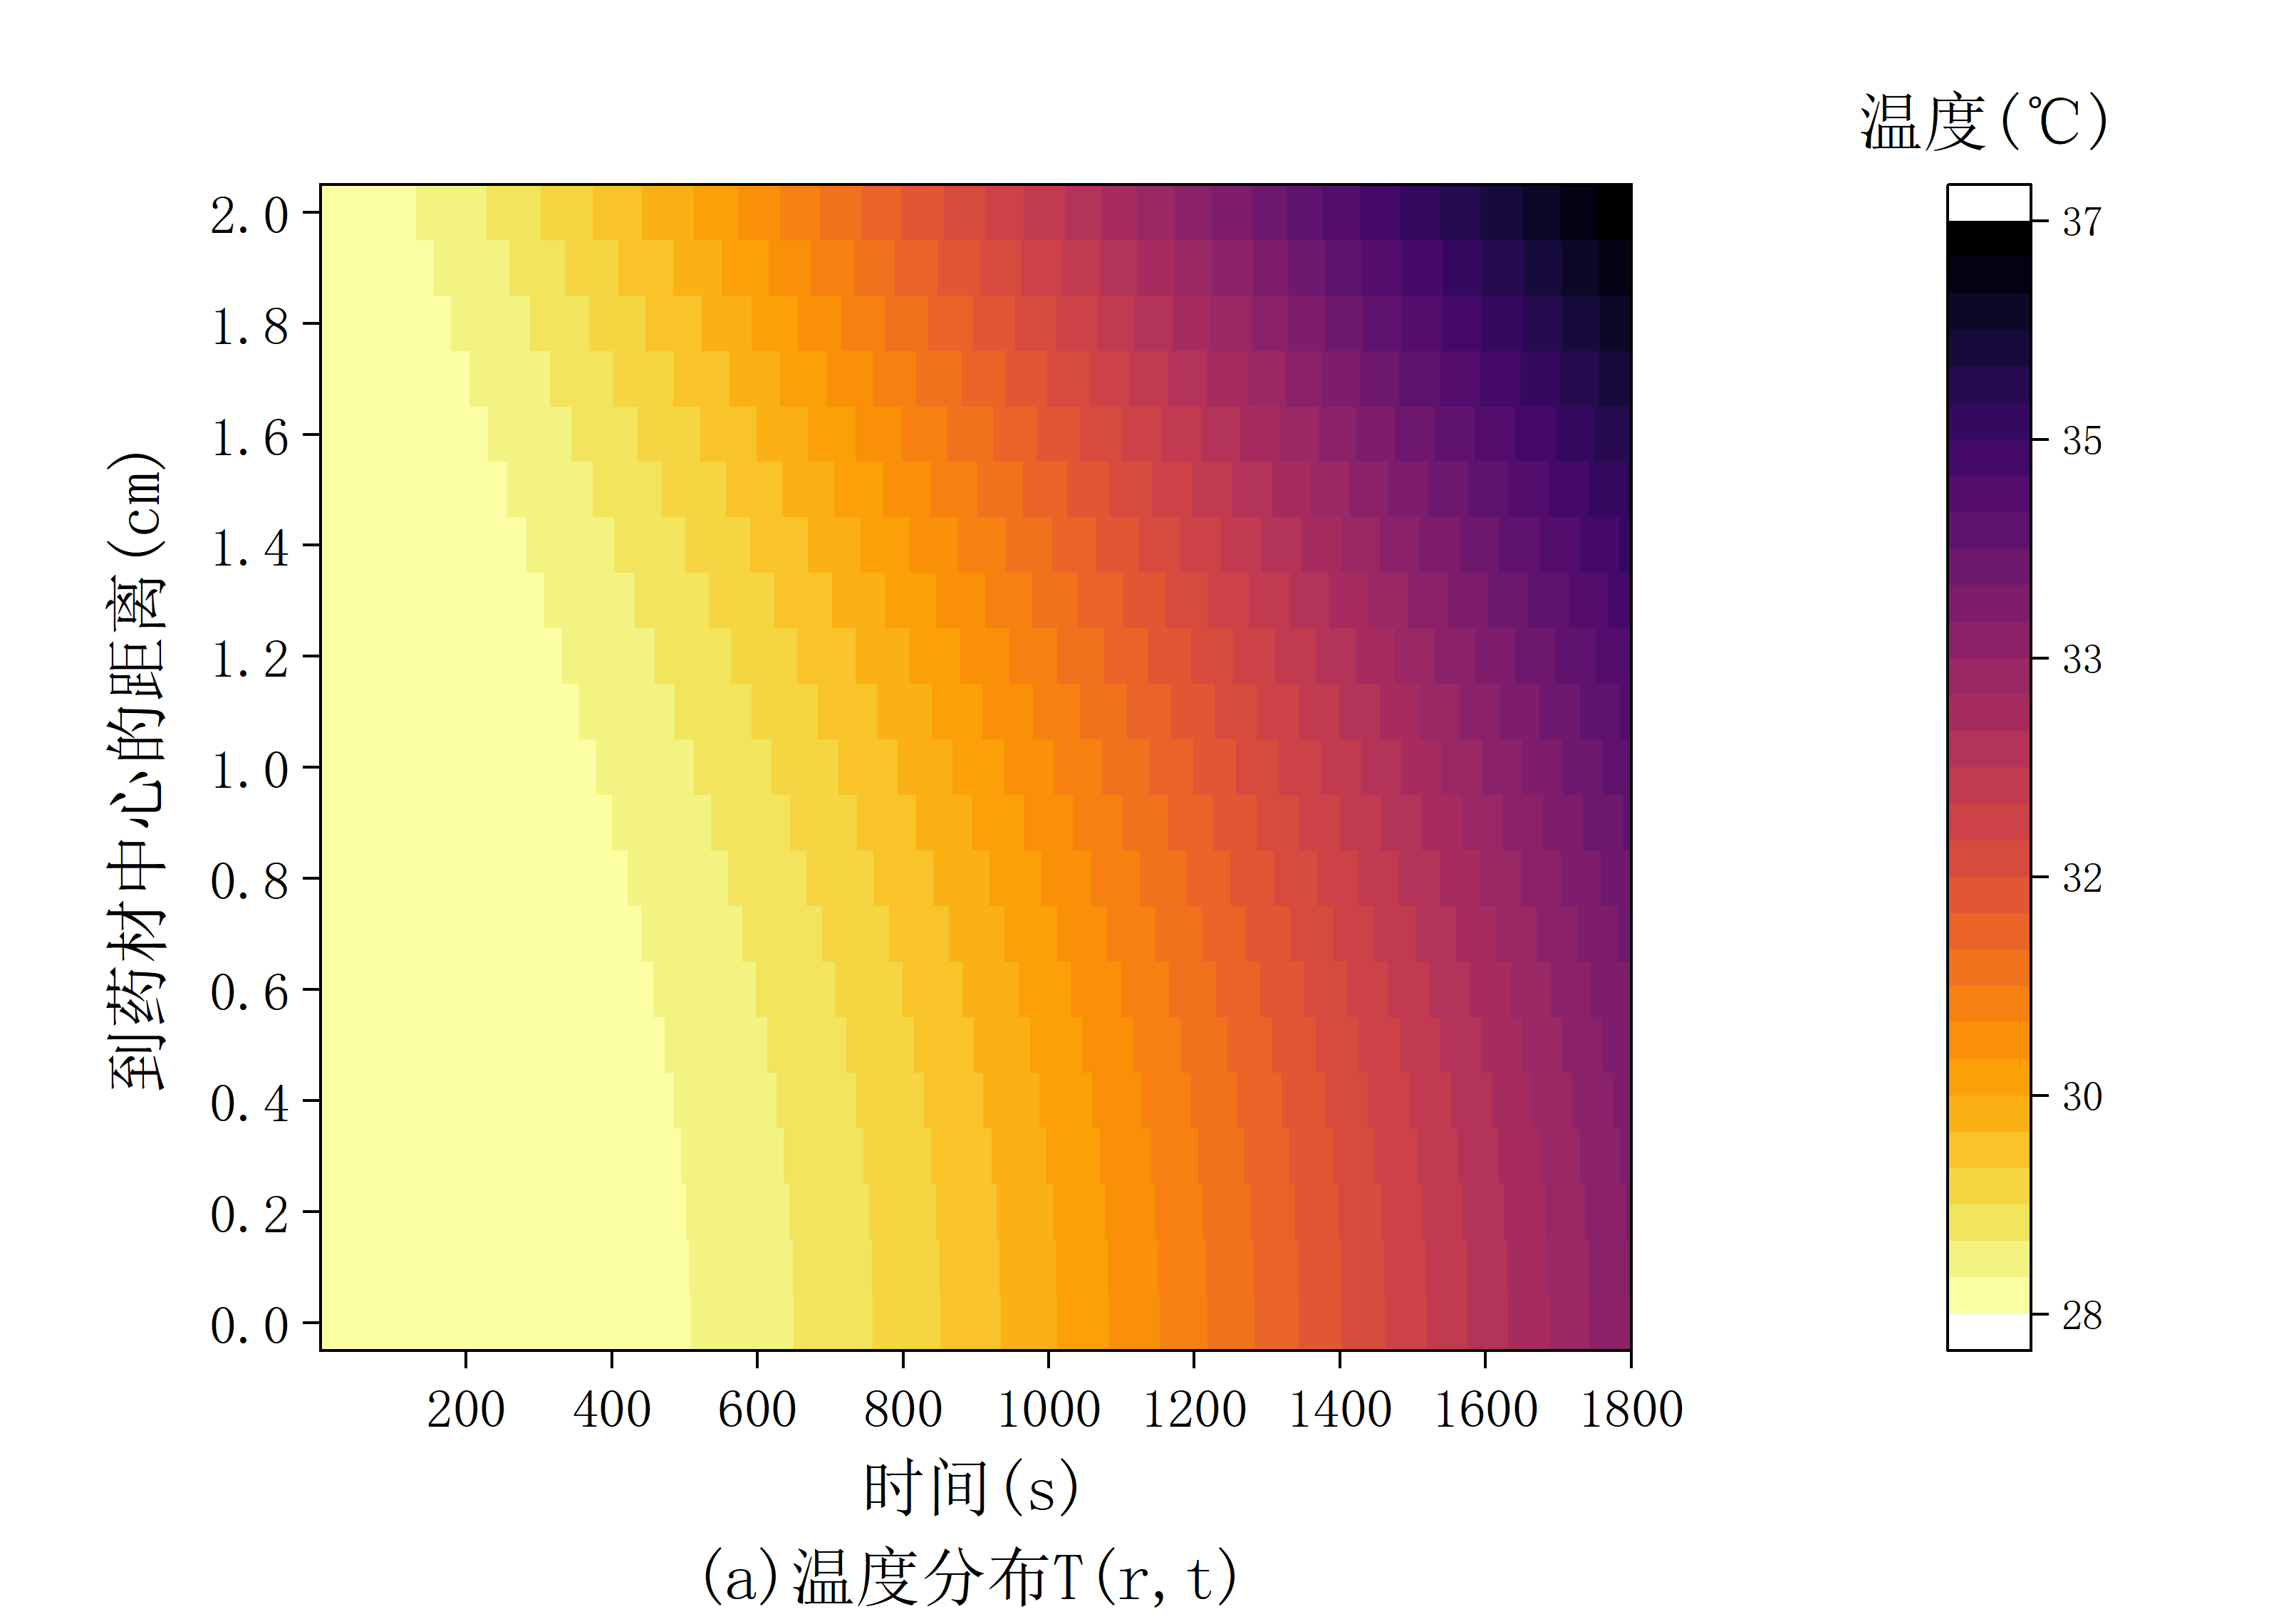
\includegraphics[trim={32.400bp 26.400bp 200.640bp 32.400bp},clip,
      height=0.400352928\unitlength]{图4(a).png}}}
  % Colorbar
  \put(0.443173632,0.053707042){\makebox(0,0)[lb]{%
    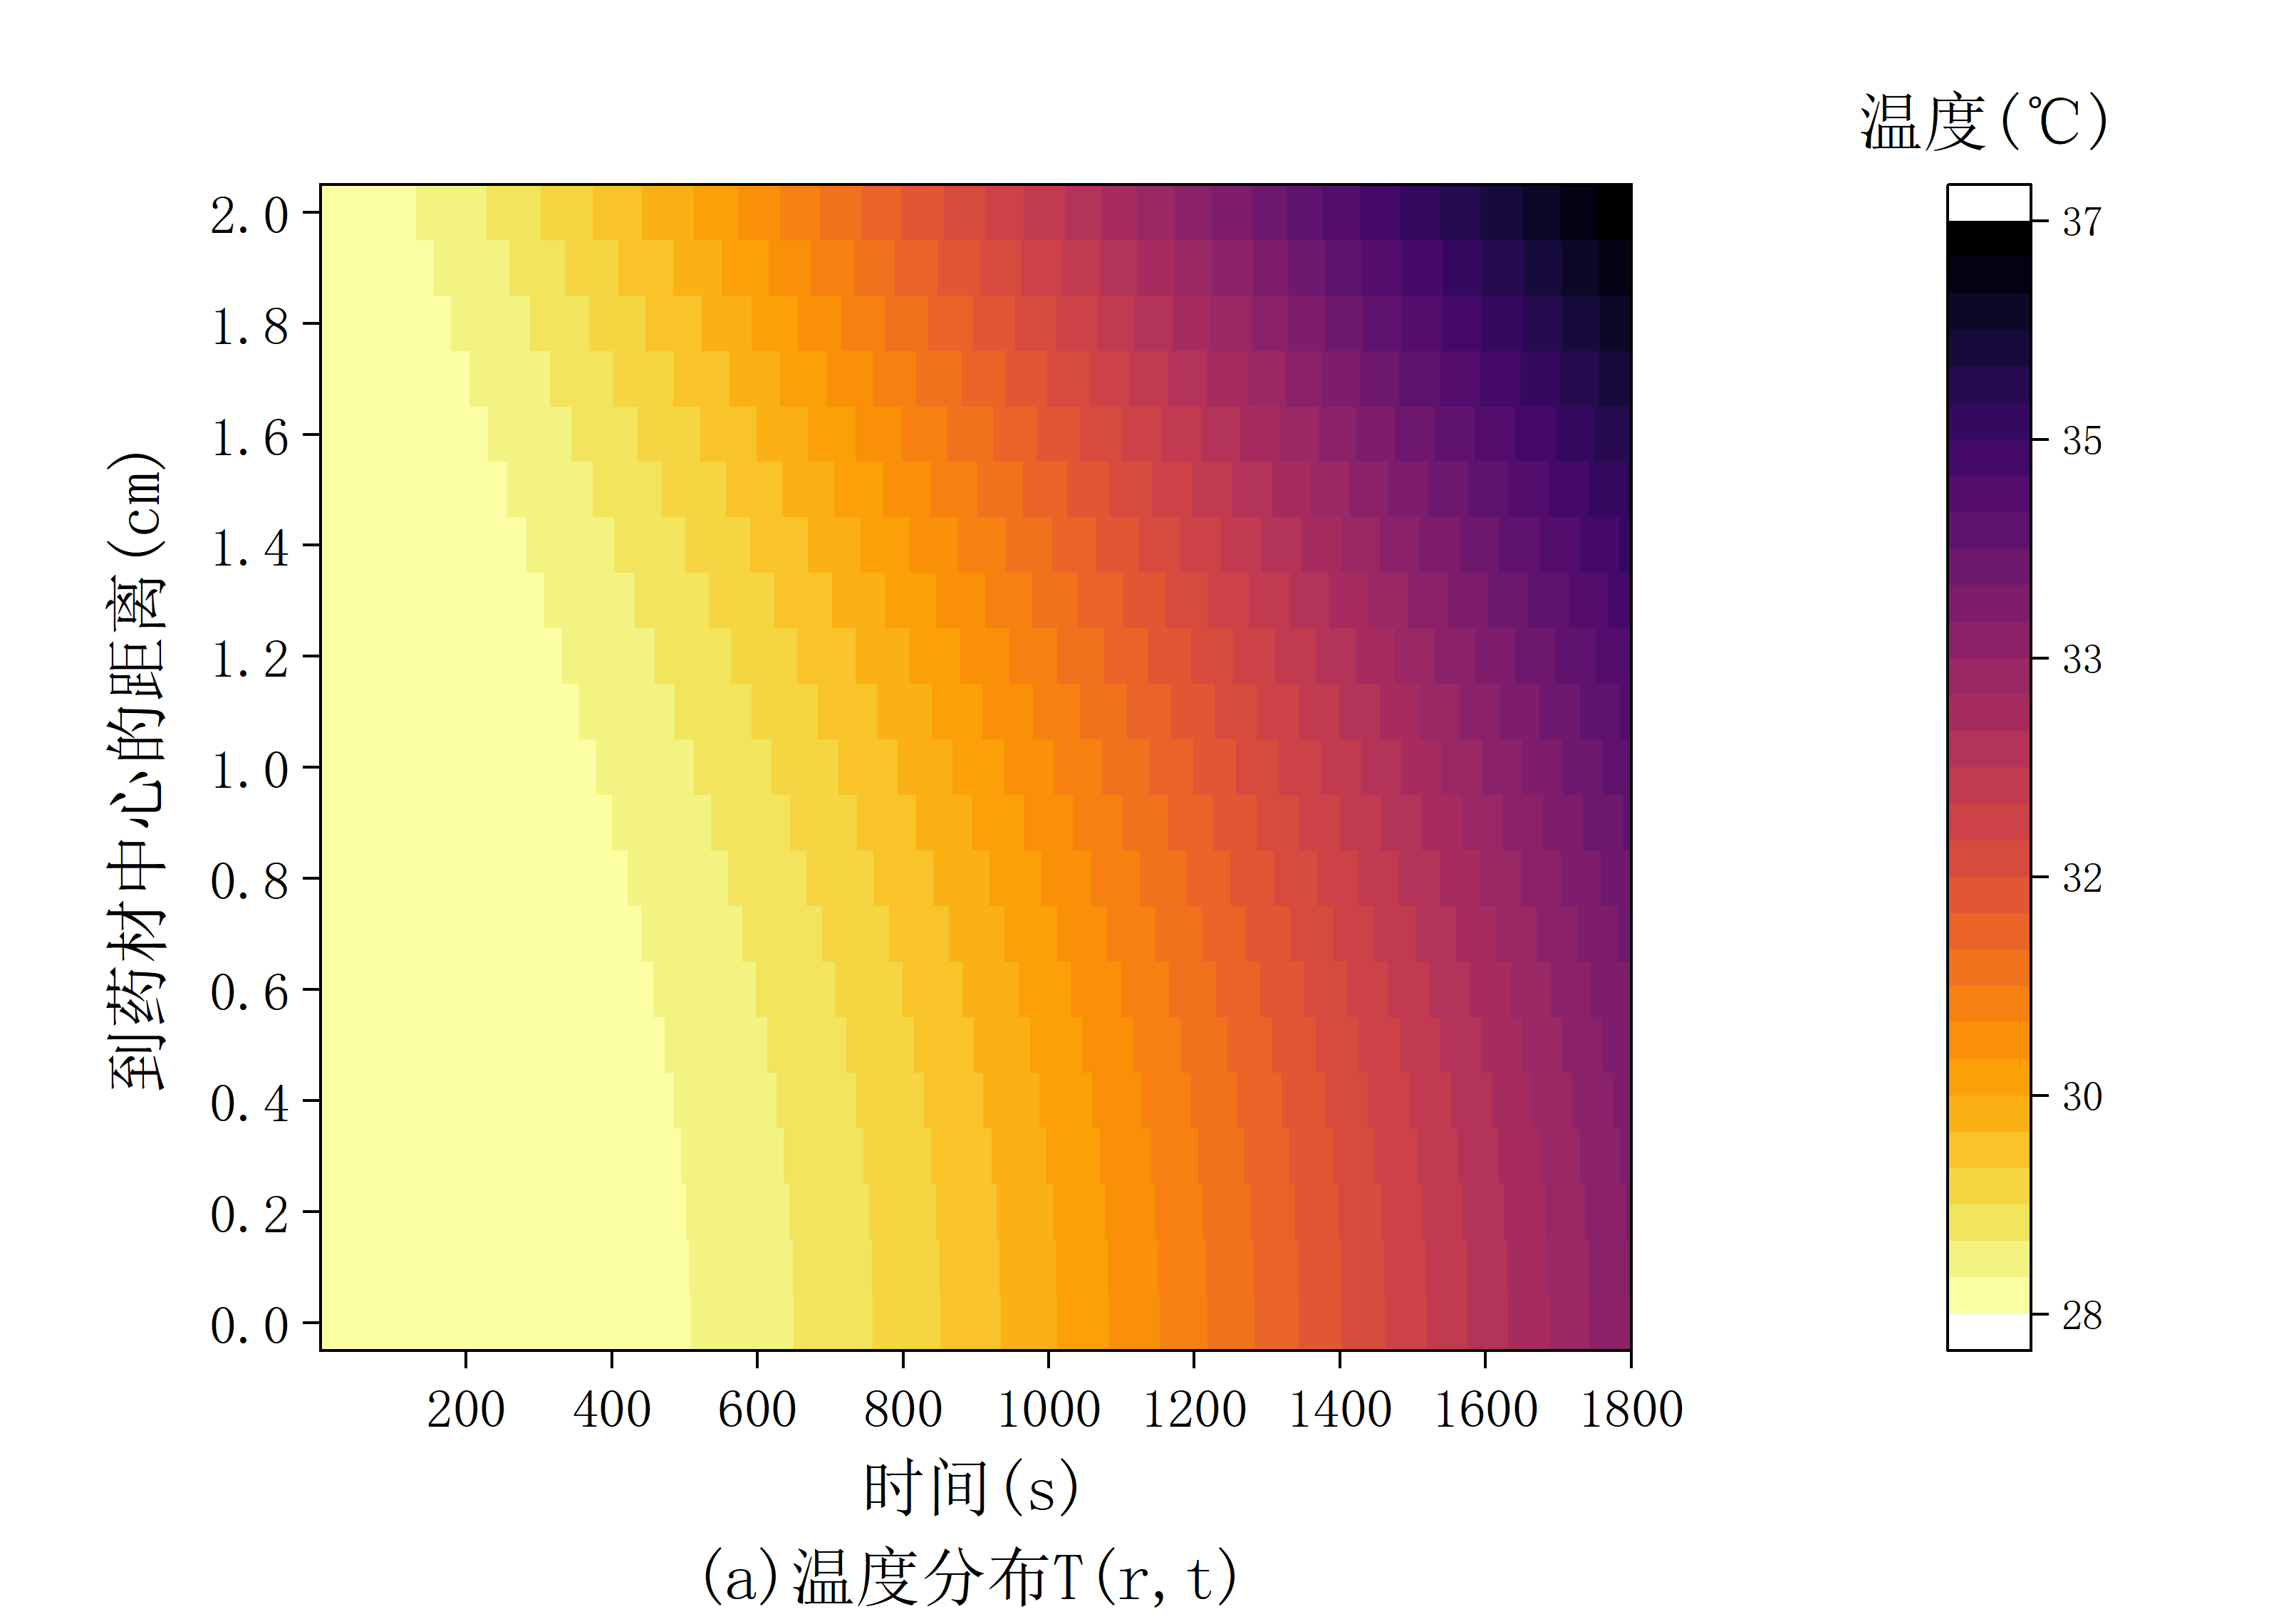
\includegraphics[trim={651.600bp 86.400bp 38.640bp 58.800bp},clip,
      height=0.329528822\unitlength]{图4(a).png}}}
  % ColorbarTitle
  \put(0.420549265,0.387170537){\makebox(0,0)[lb]{%
    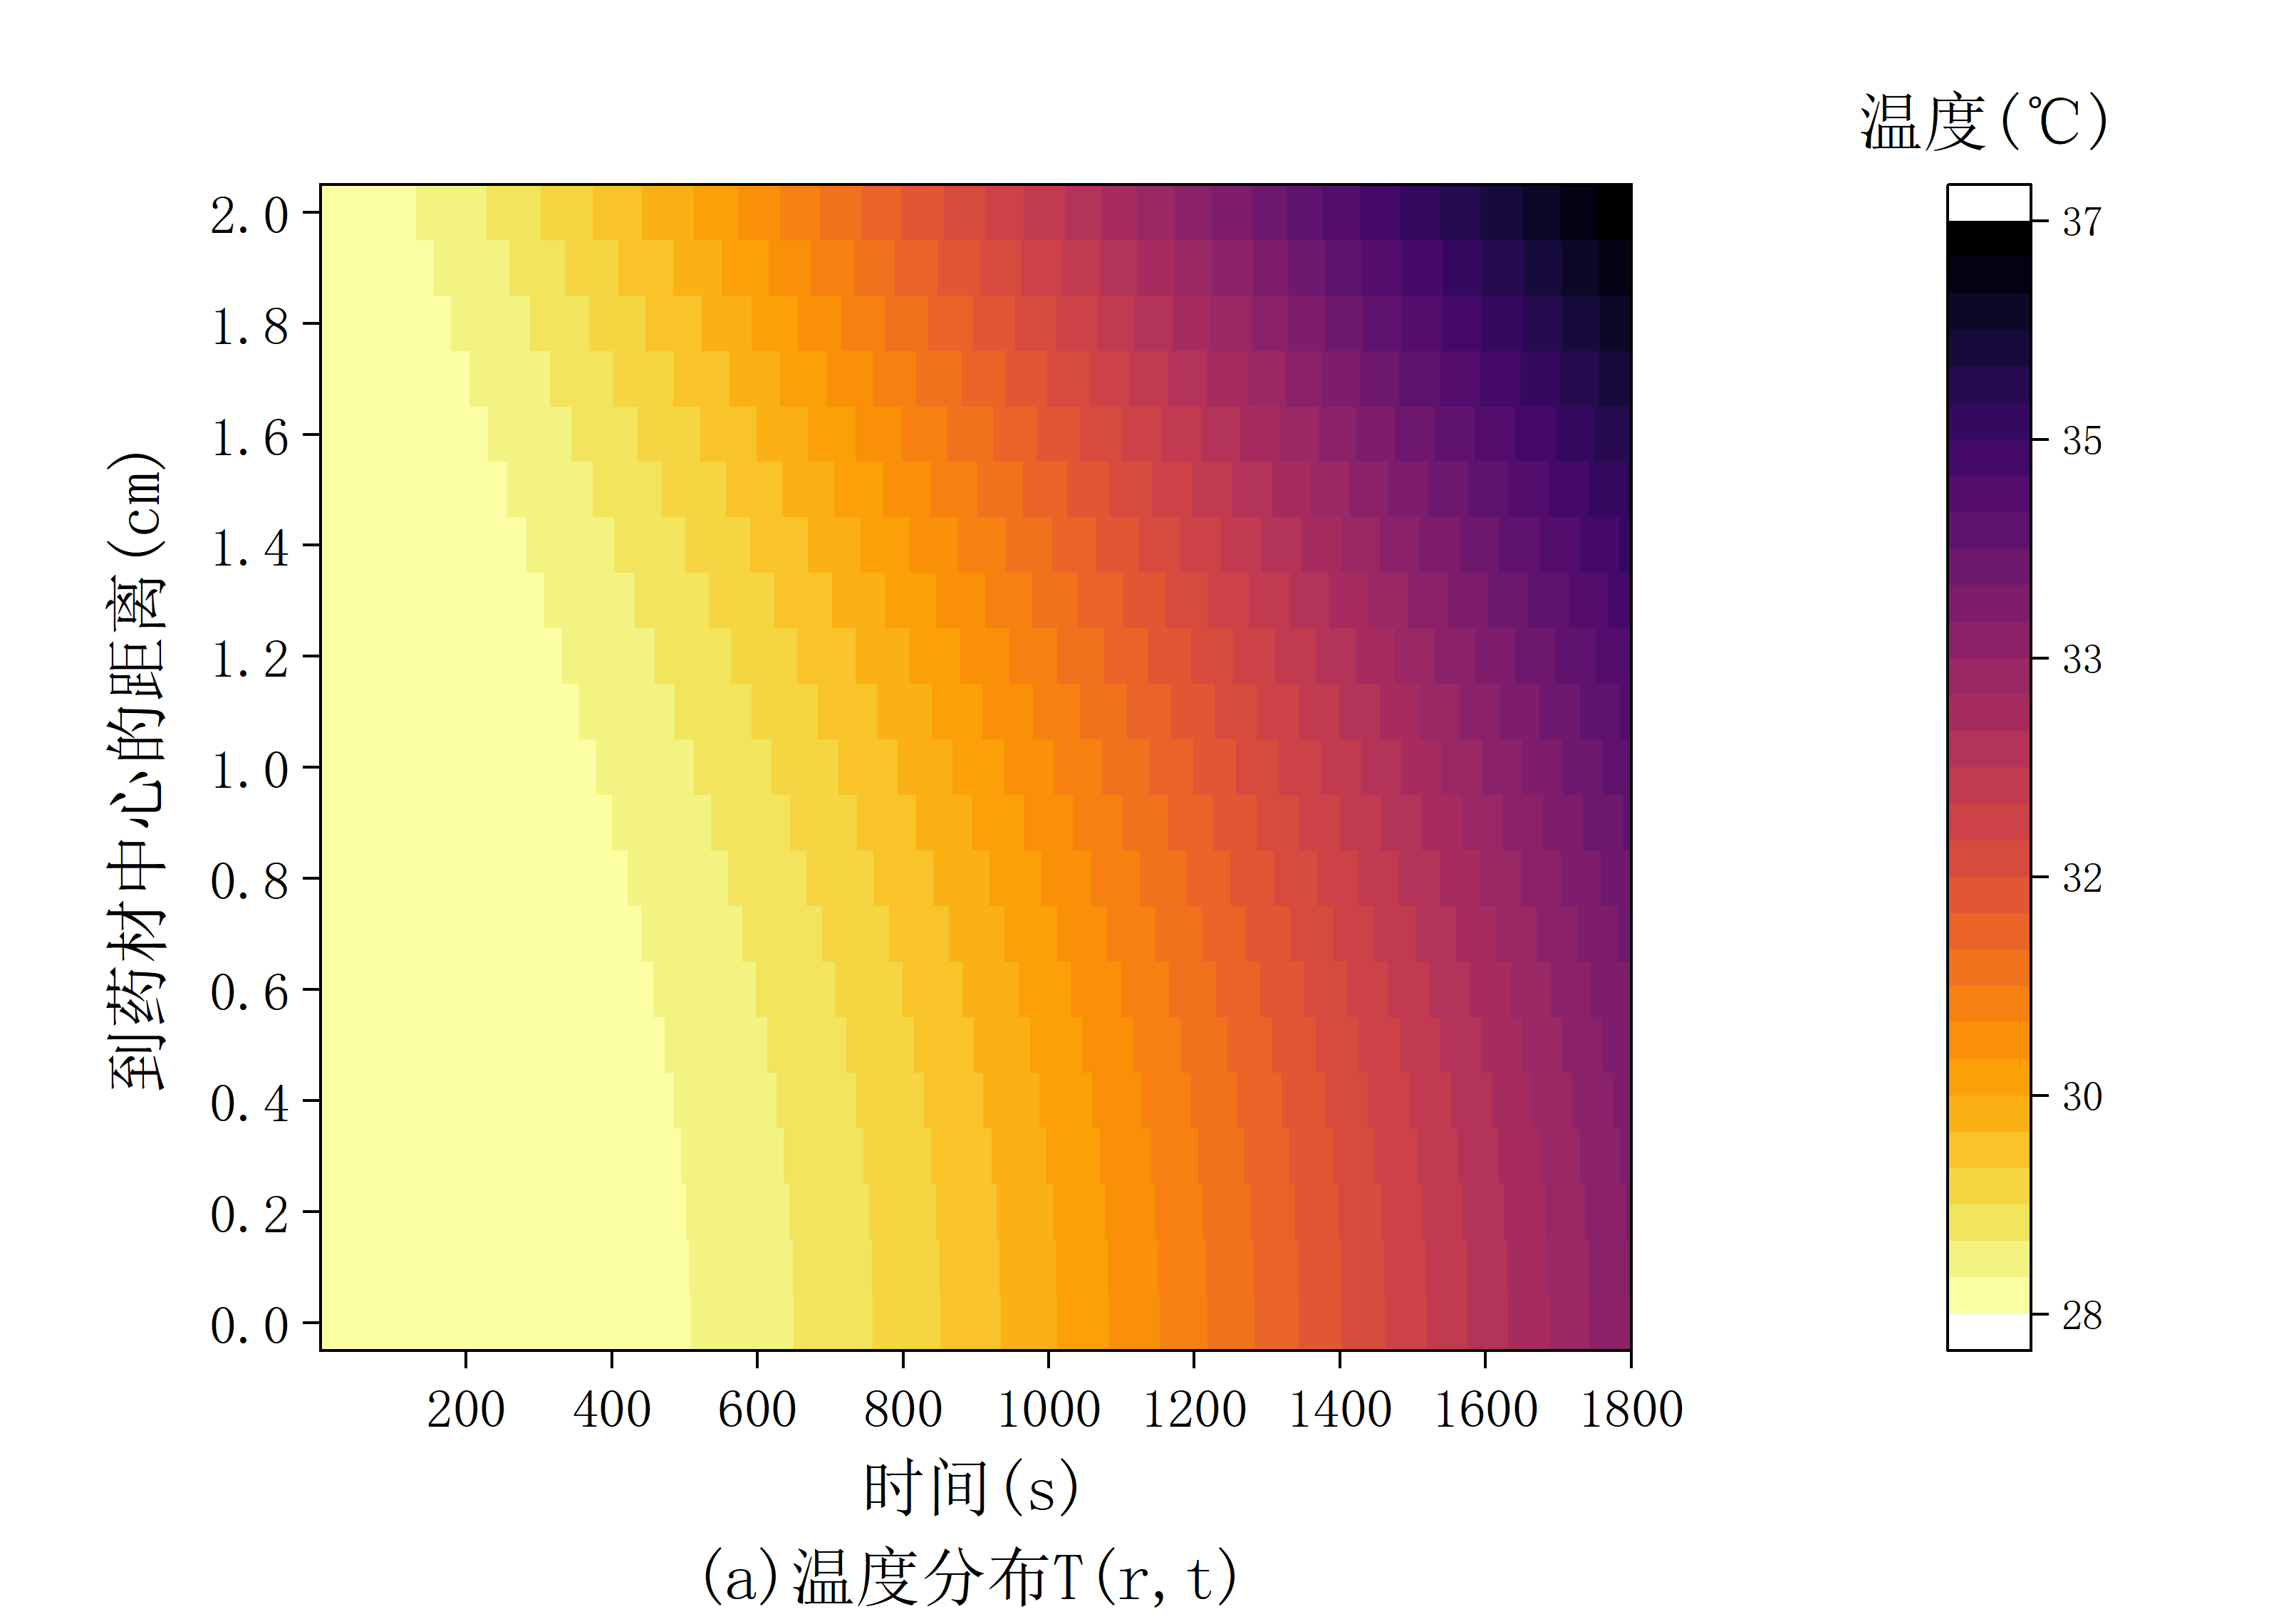
\includegraphics[trim={624.000bp 493.200bp 59.040bp 27.600bp},clip,
      height=0.021640699\unitlength]{图4(a).png}}}
  % B：仅指定高度，保持原PNG比例；向左利用空白间距。
  \put(0.513589096,0.013349051){\makebox(0,0)[lb]{%
    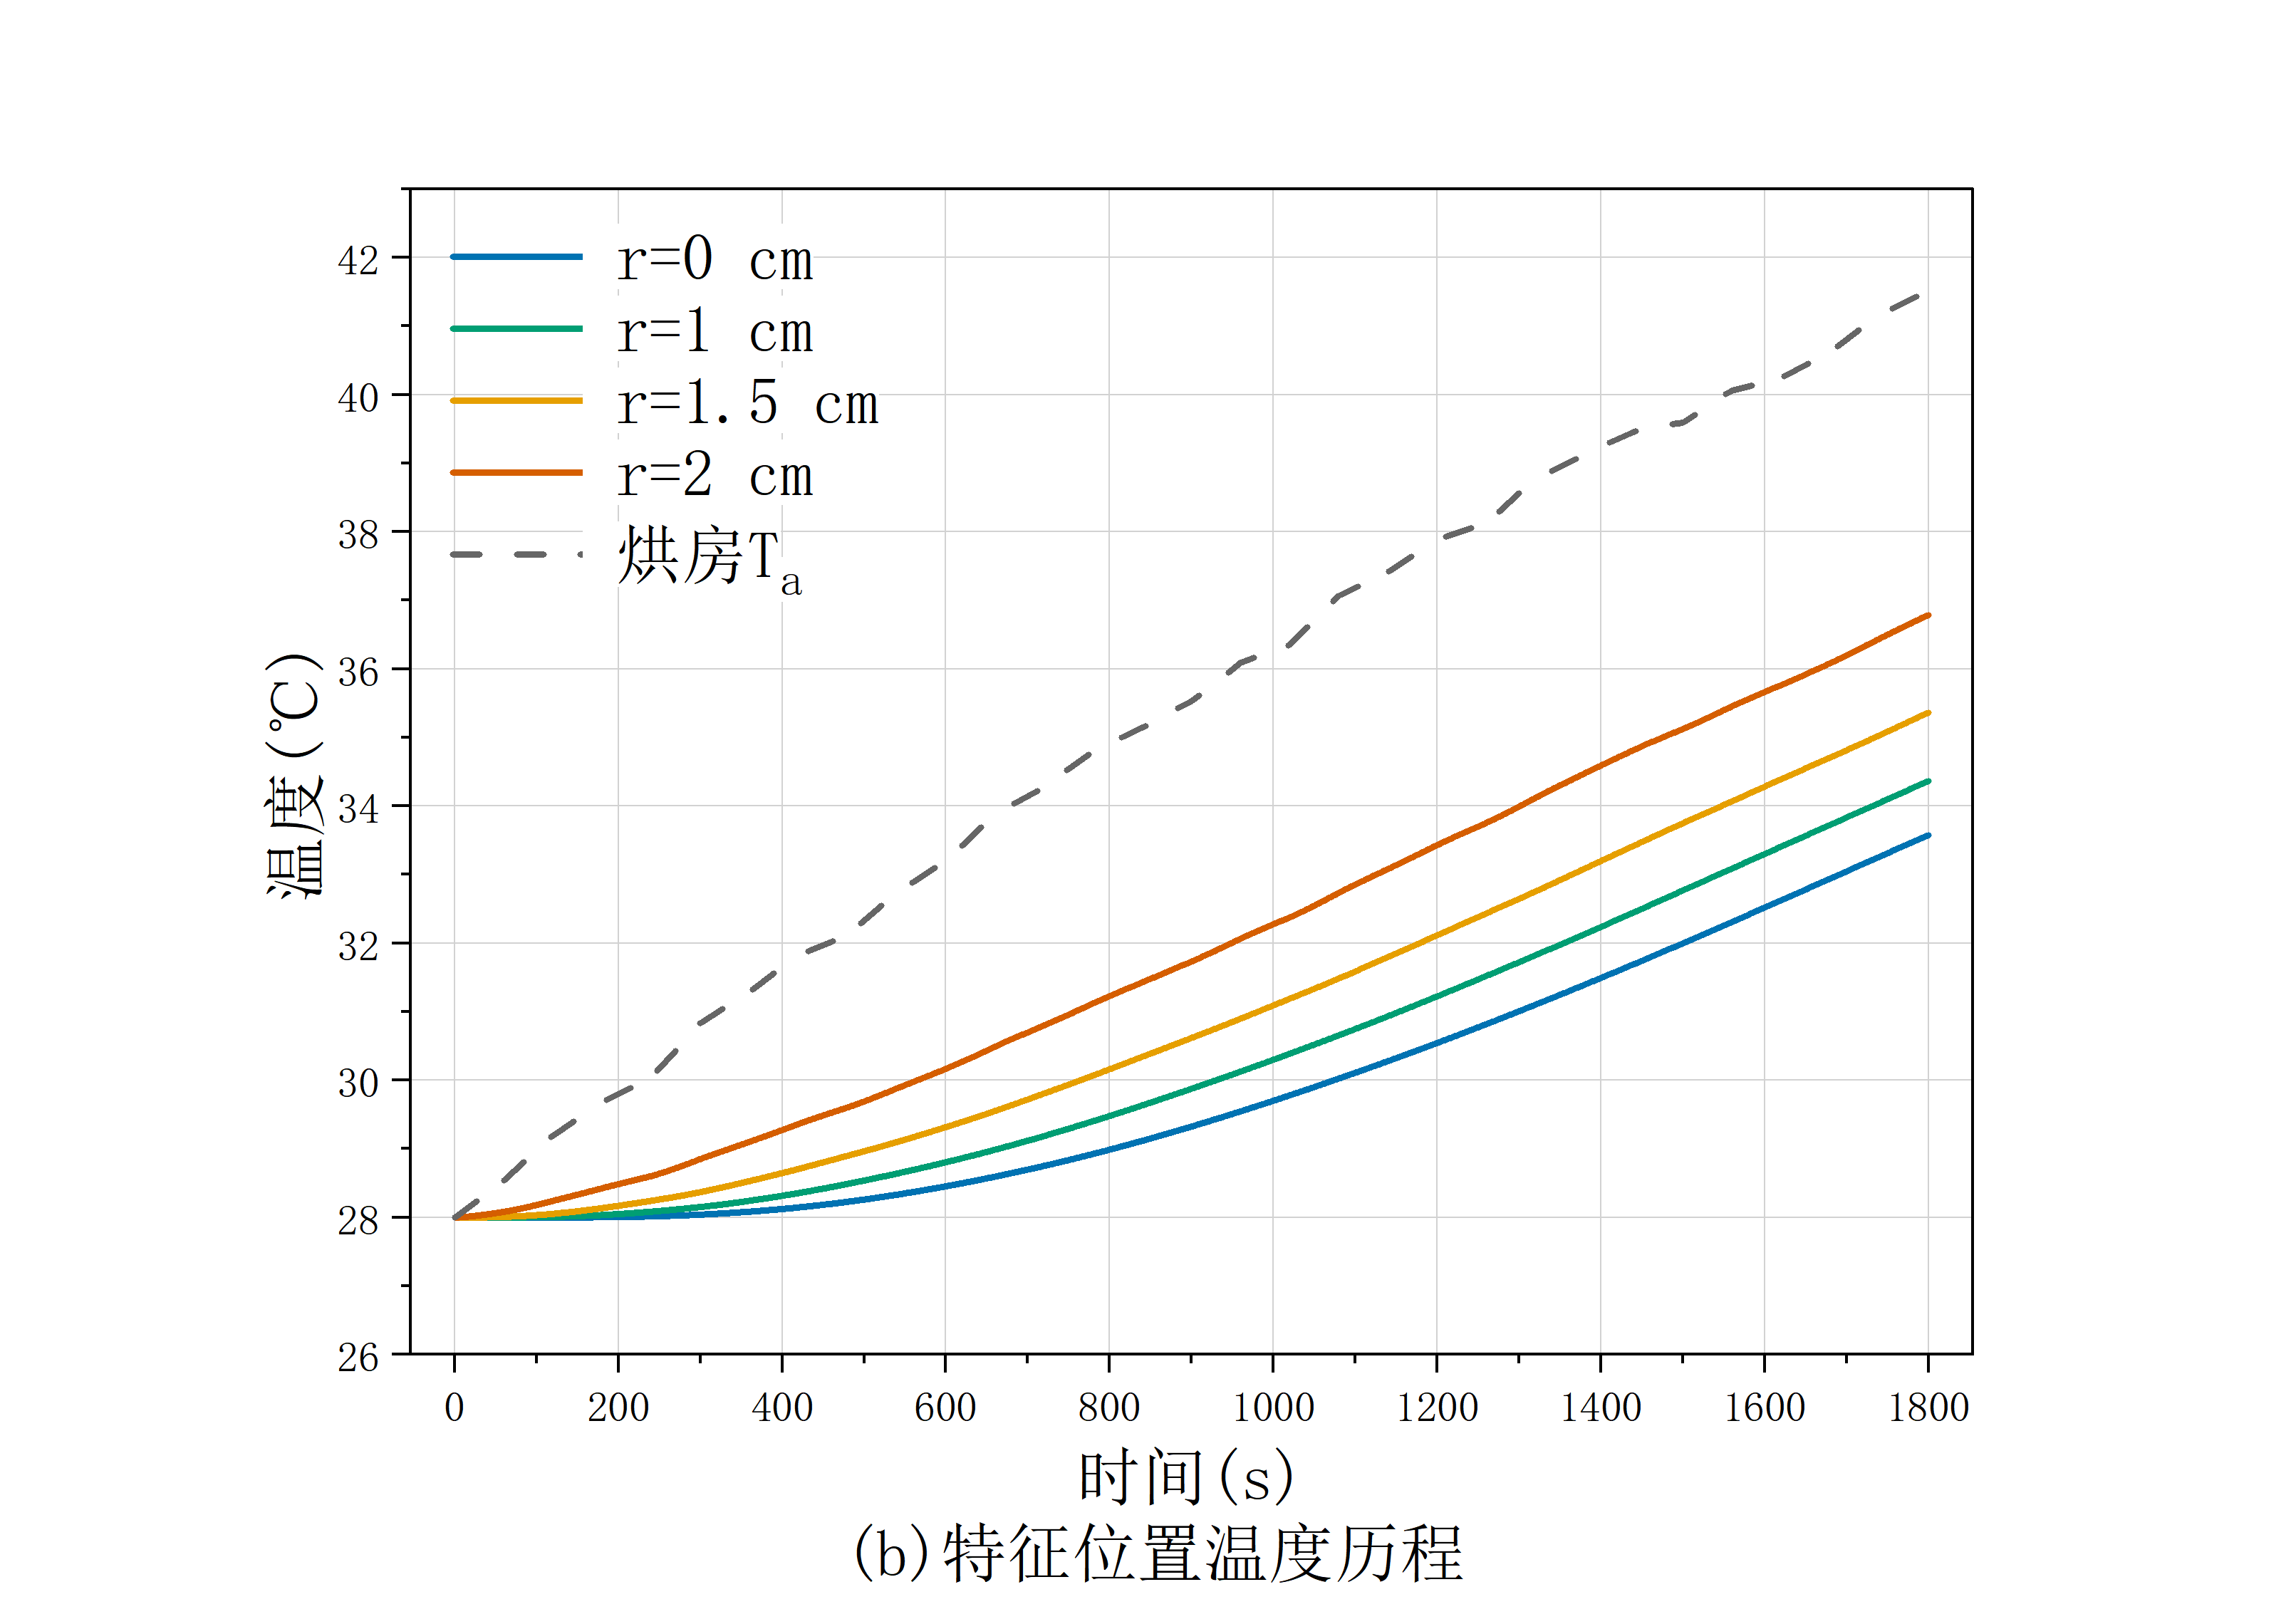
\includegraphics[trim={85.200bp 36.000bp 102.240bp 34.800bp},clip,
      height=0.390754948\unitlength]{图4(b).png}}}
\end{picture}
\caption{问题一温度场及特征位置温度历程}
\label{fig:p1-temperature}
\end{figure}

环境热量经表面对流输入，再由径向导热向内传递，有限的表面交换与内部导热能力形成上述温差。
因此，\textbf{30分钟时内部温度尚未均匀，药材与环境也未达到热平衡}。

\subsubsection{表层失水与热湿响应差异}

同期表面含水率由$2.55\cunit$降至$1.5102\cunit$，下降约$40.78\%$，
中心在表格显示精度下仍为$2.5500\cunit$。
图\ref{fig:p1-moisture}的径向剖面在内部平缓、近表面明显下降，
表明\textbf{前30分钟的显著失水主要集中于外层}。

\begin{figure}[!htbp]
\centering
% 保持原图4的0.98\textwidth宽度及264.62175/636.93875高宽比。
% 裁去白边并收紧(a)主图与色条的间距，完整保留两行色条标题。
% trim按源PNG的300 dpi换算；各部分仅指定高度，以保持原始比例。
\setlength{\unitlength}{0.98\textwidth}
\begin{picture}(1,0.415458708)
  % (a)水分场及坐标轴。
  \put(0.016642117,0.001726623){\makebox(0,0)[lb]{%
    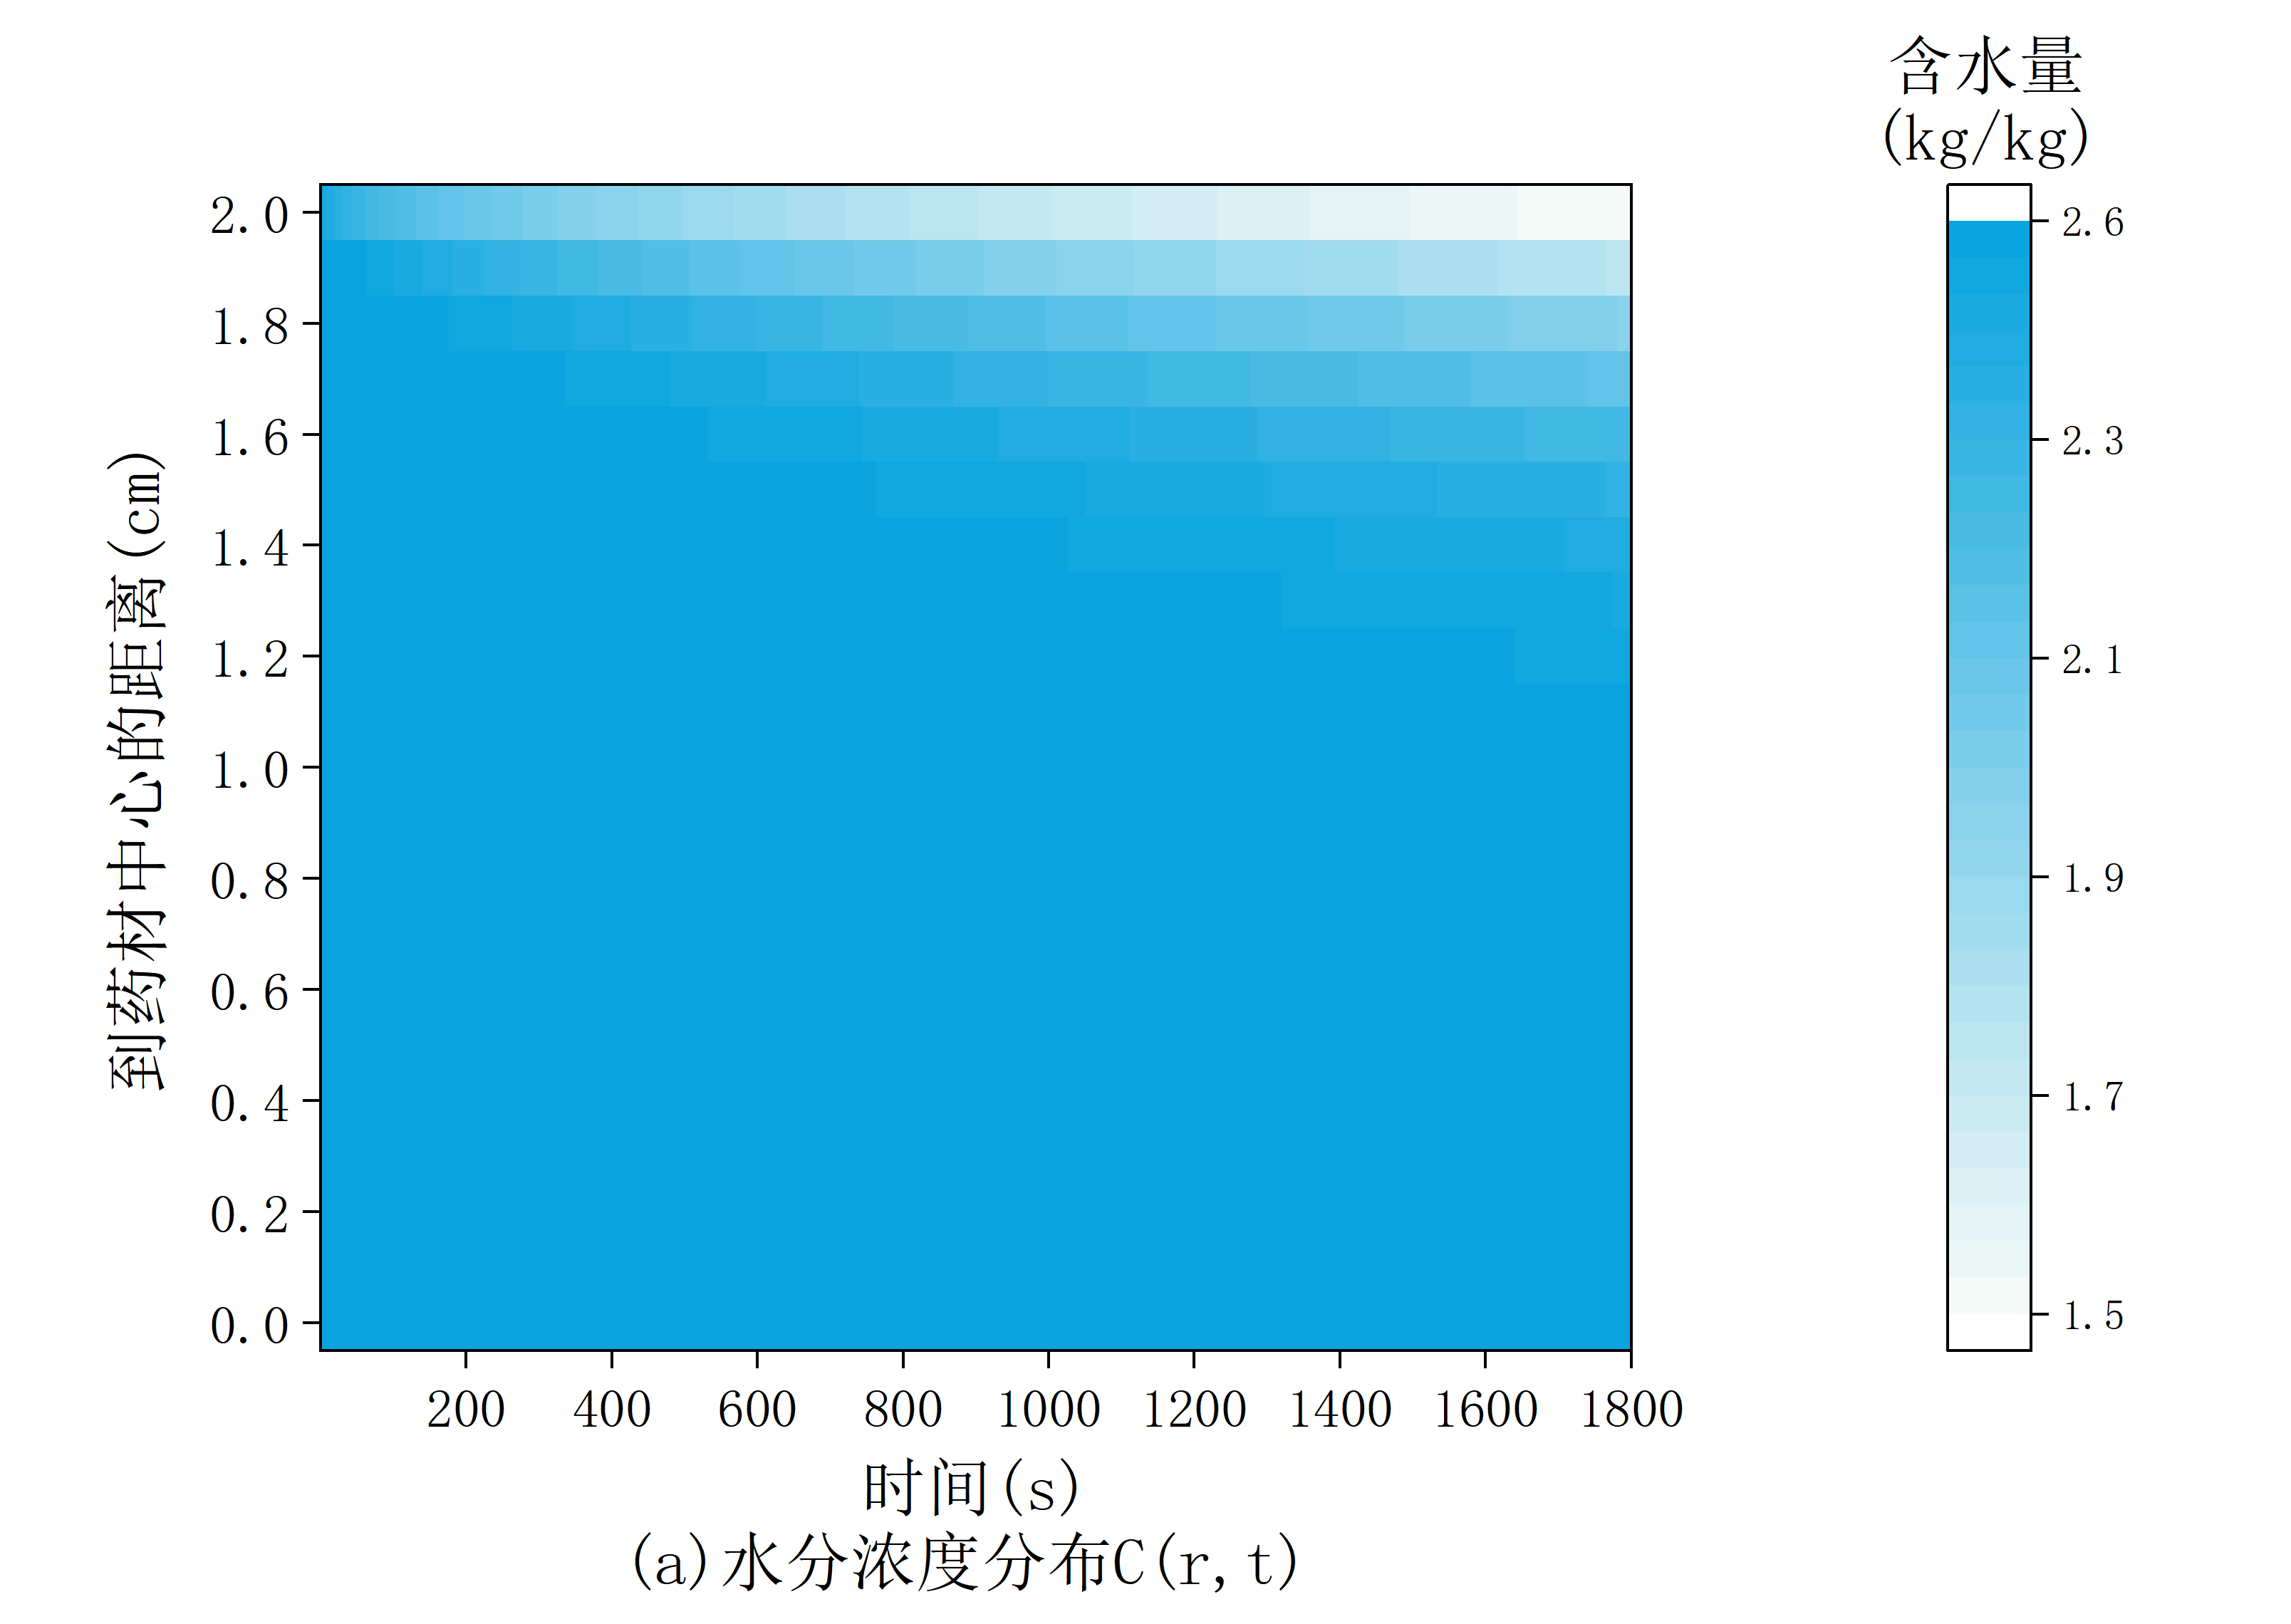
\includegraphics[trim={32.400bp 26.400bp 200.640bp 34.800bp},clip,
      height=0.392417307\unitlength]{图5(a).png}}}
  % (a)色条及其两行标题，与主图按相同比例缩放；分开裁剪避免白边覆盖主轴。
  \put(0.439628404,0.050173204){\makebox(0,0)[lb]{%
    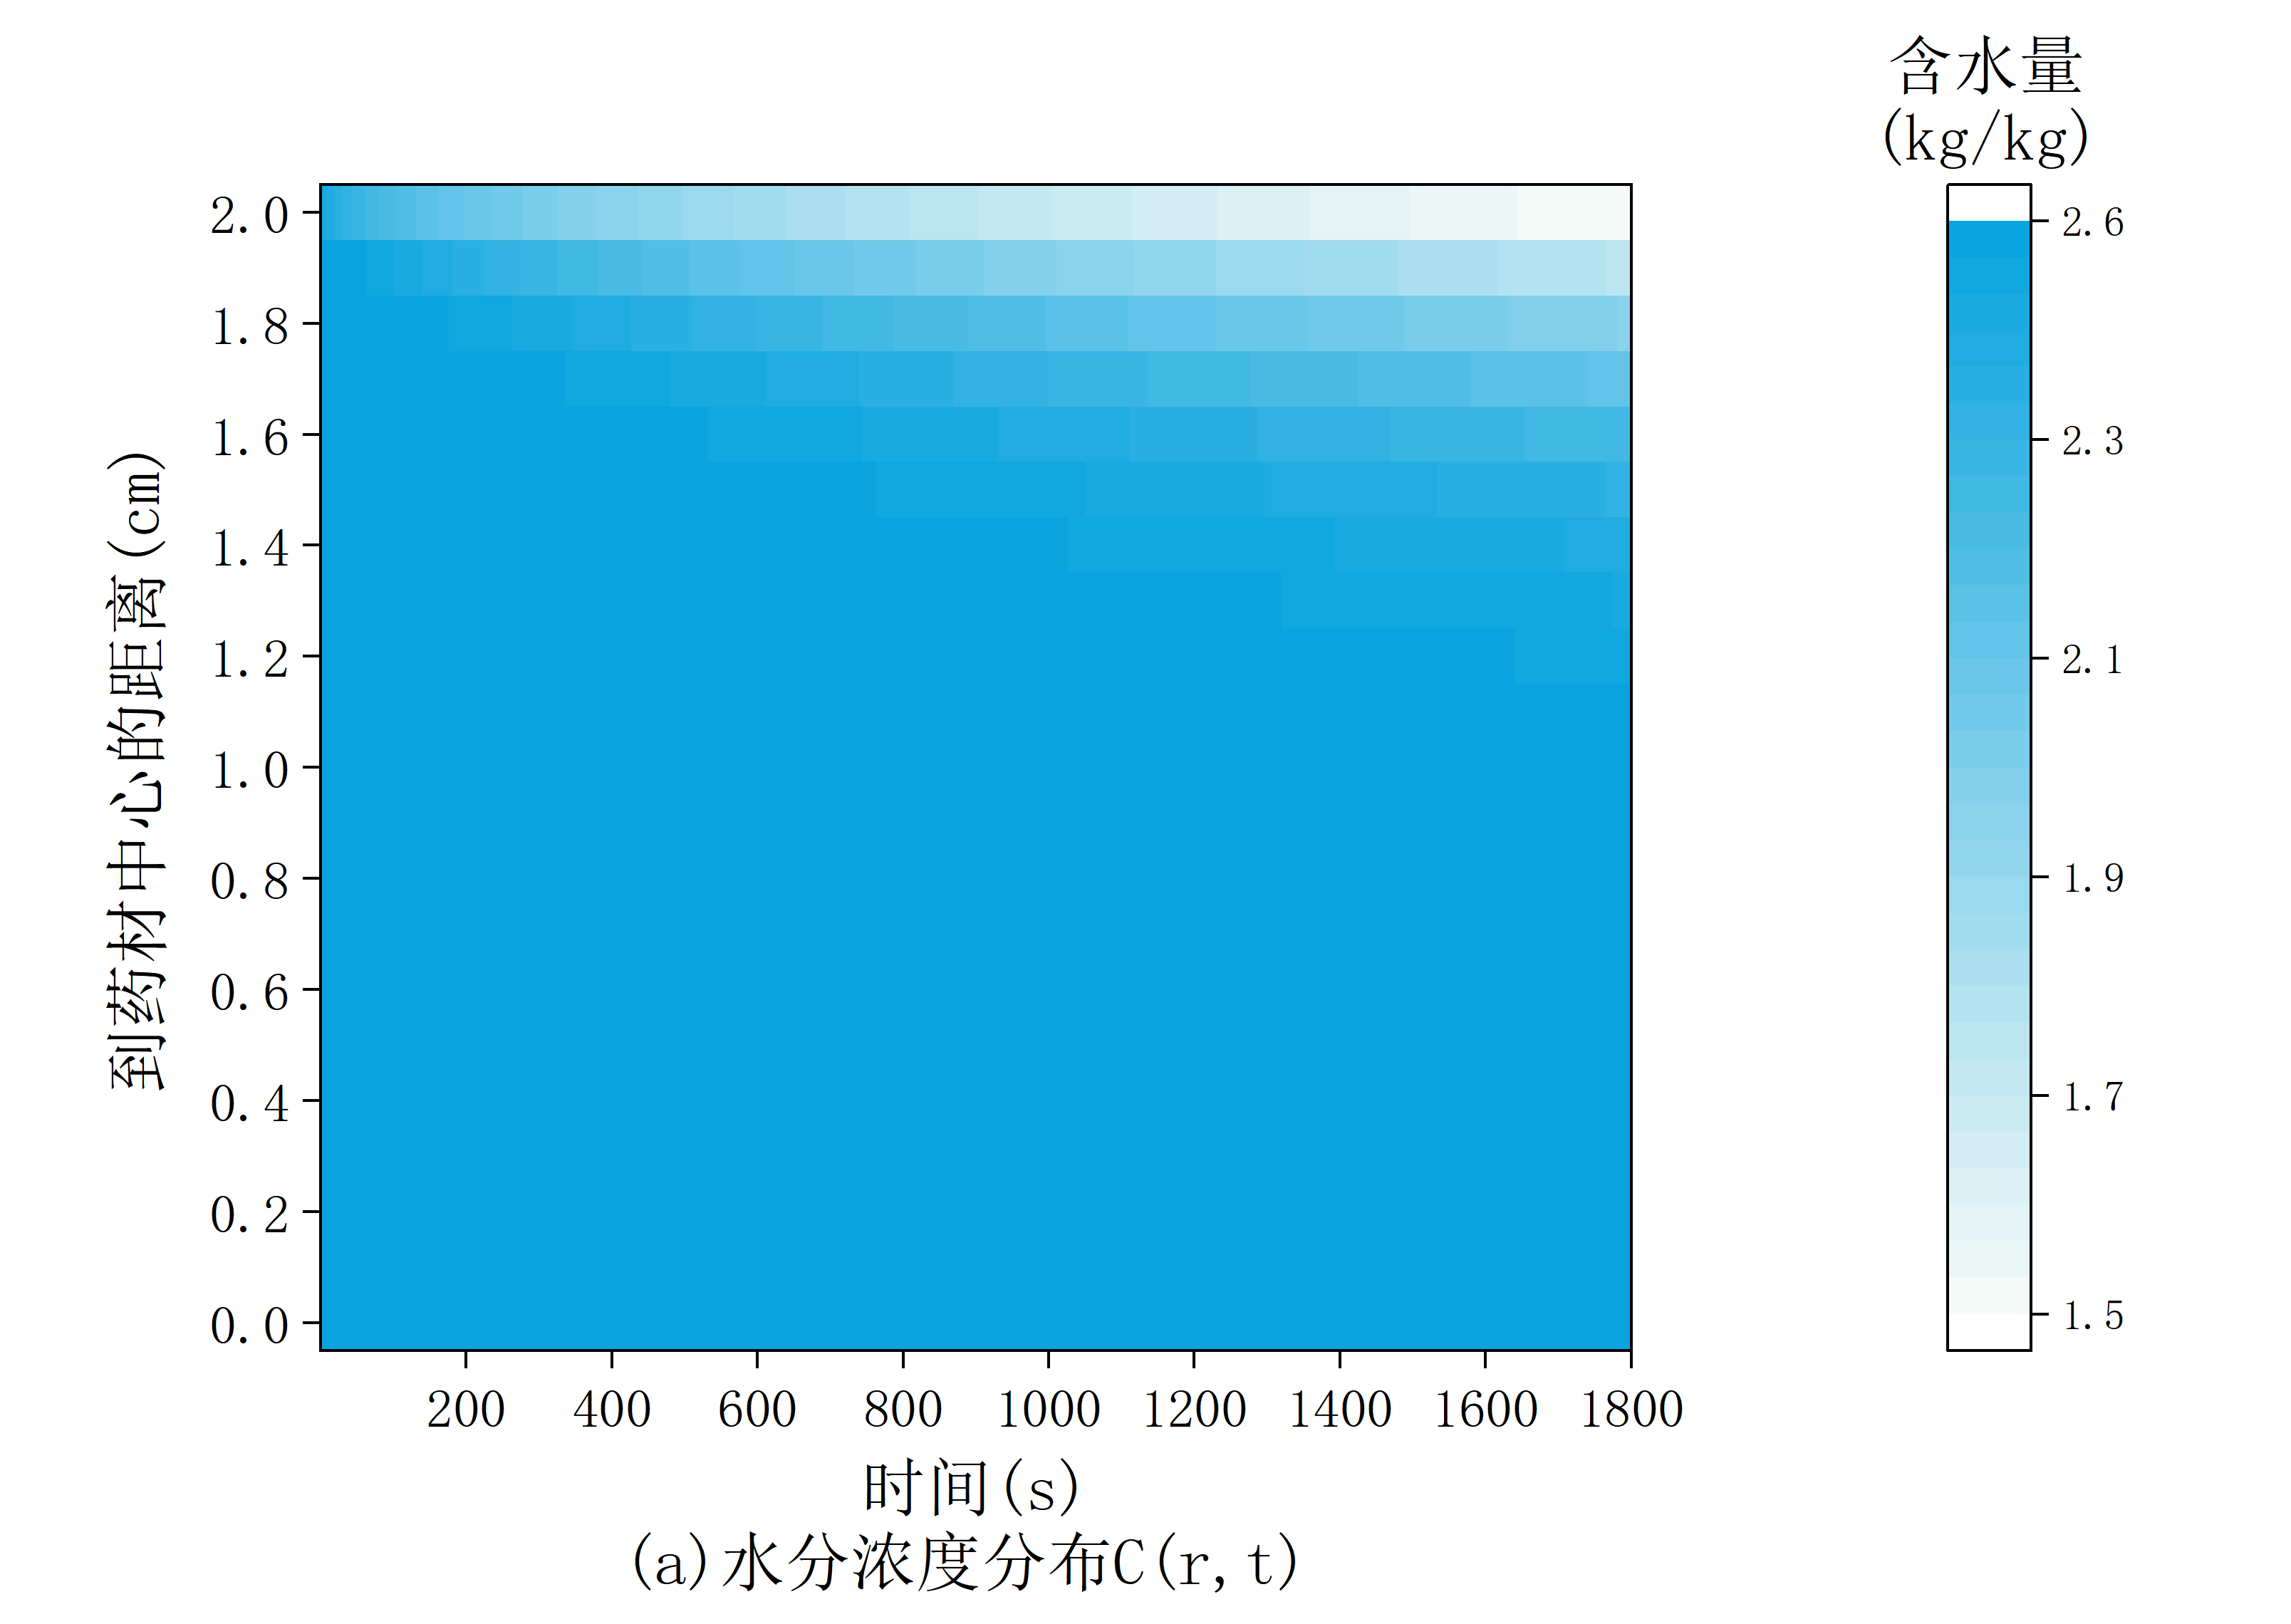
\includegraphics[trim={651.600bp 86.400bp 38.640bp 58.800bp},clip,
      height=0.324592094\unitlength]{图5(a).png}}}
  \put(0.424125498,0.374765298){\makebox(0,0)[lb]{%
    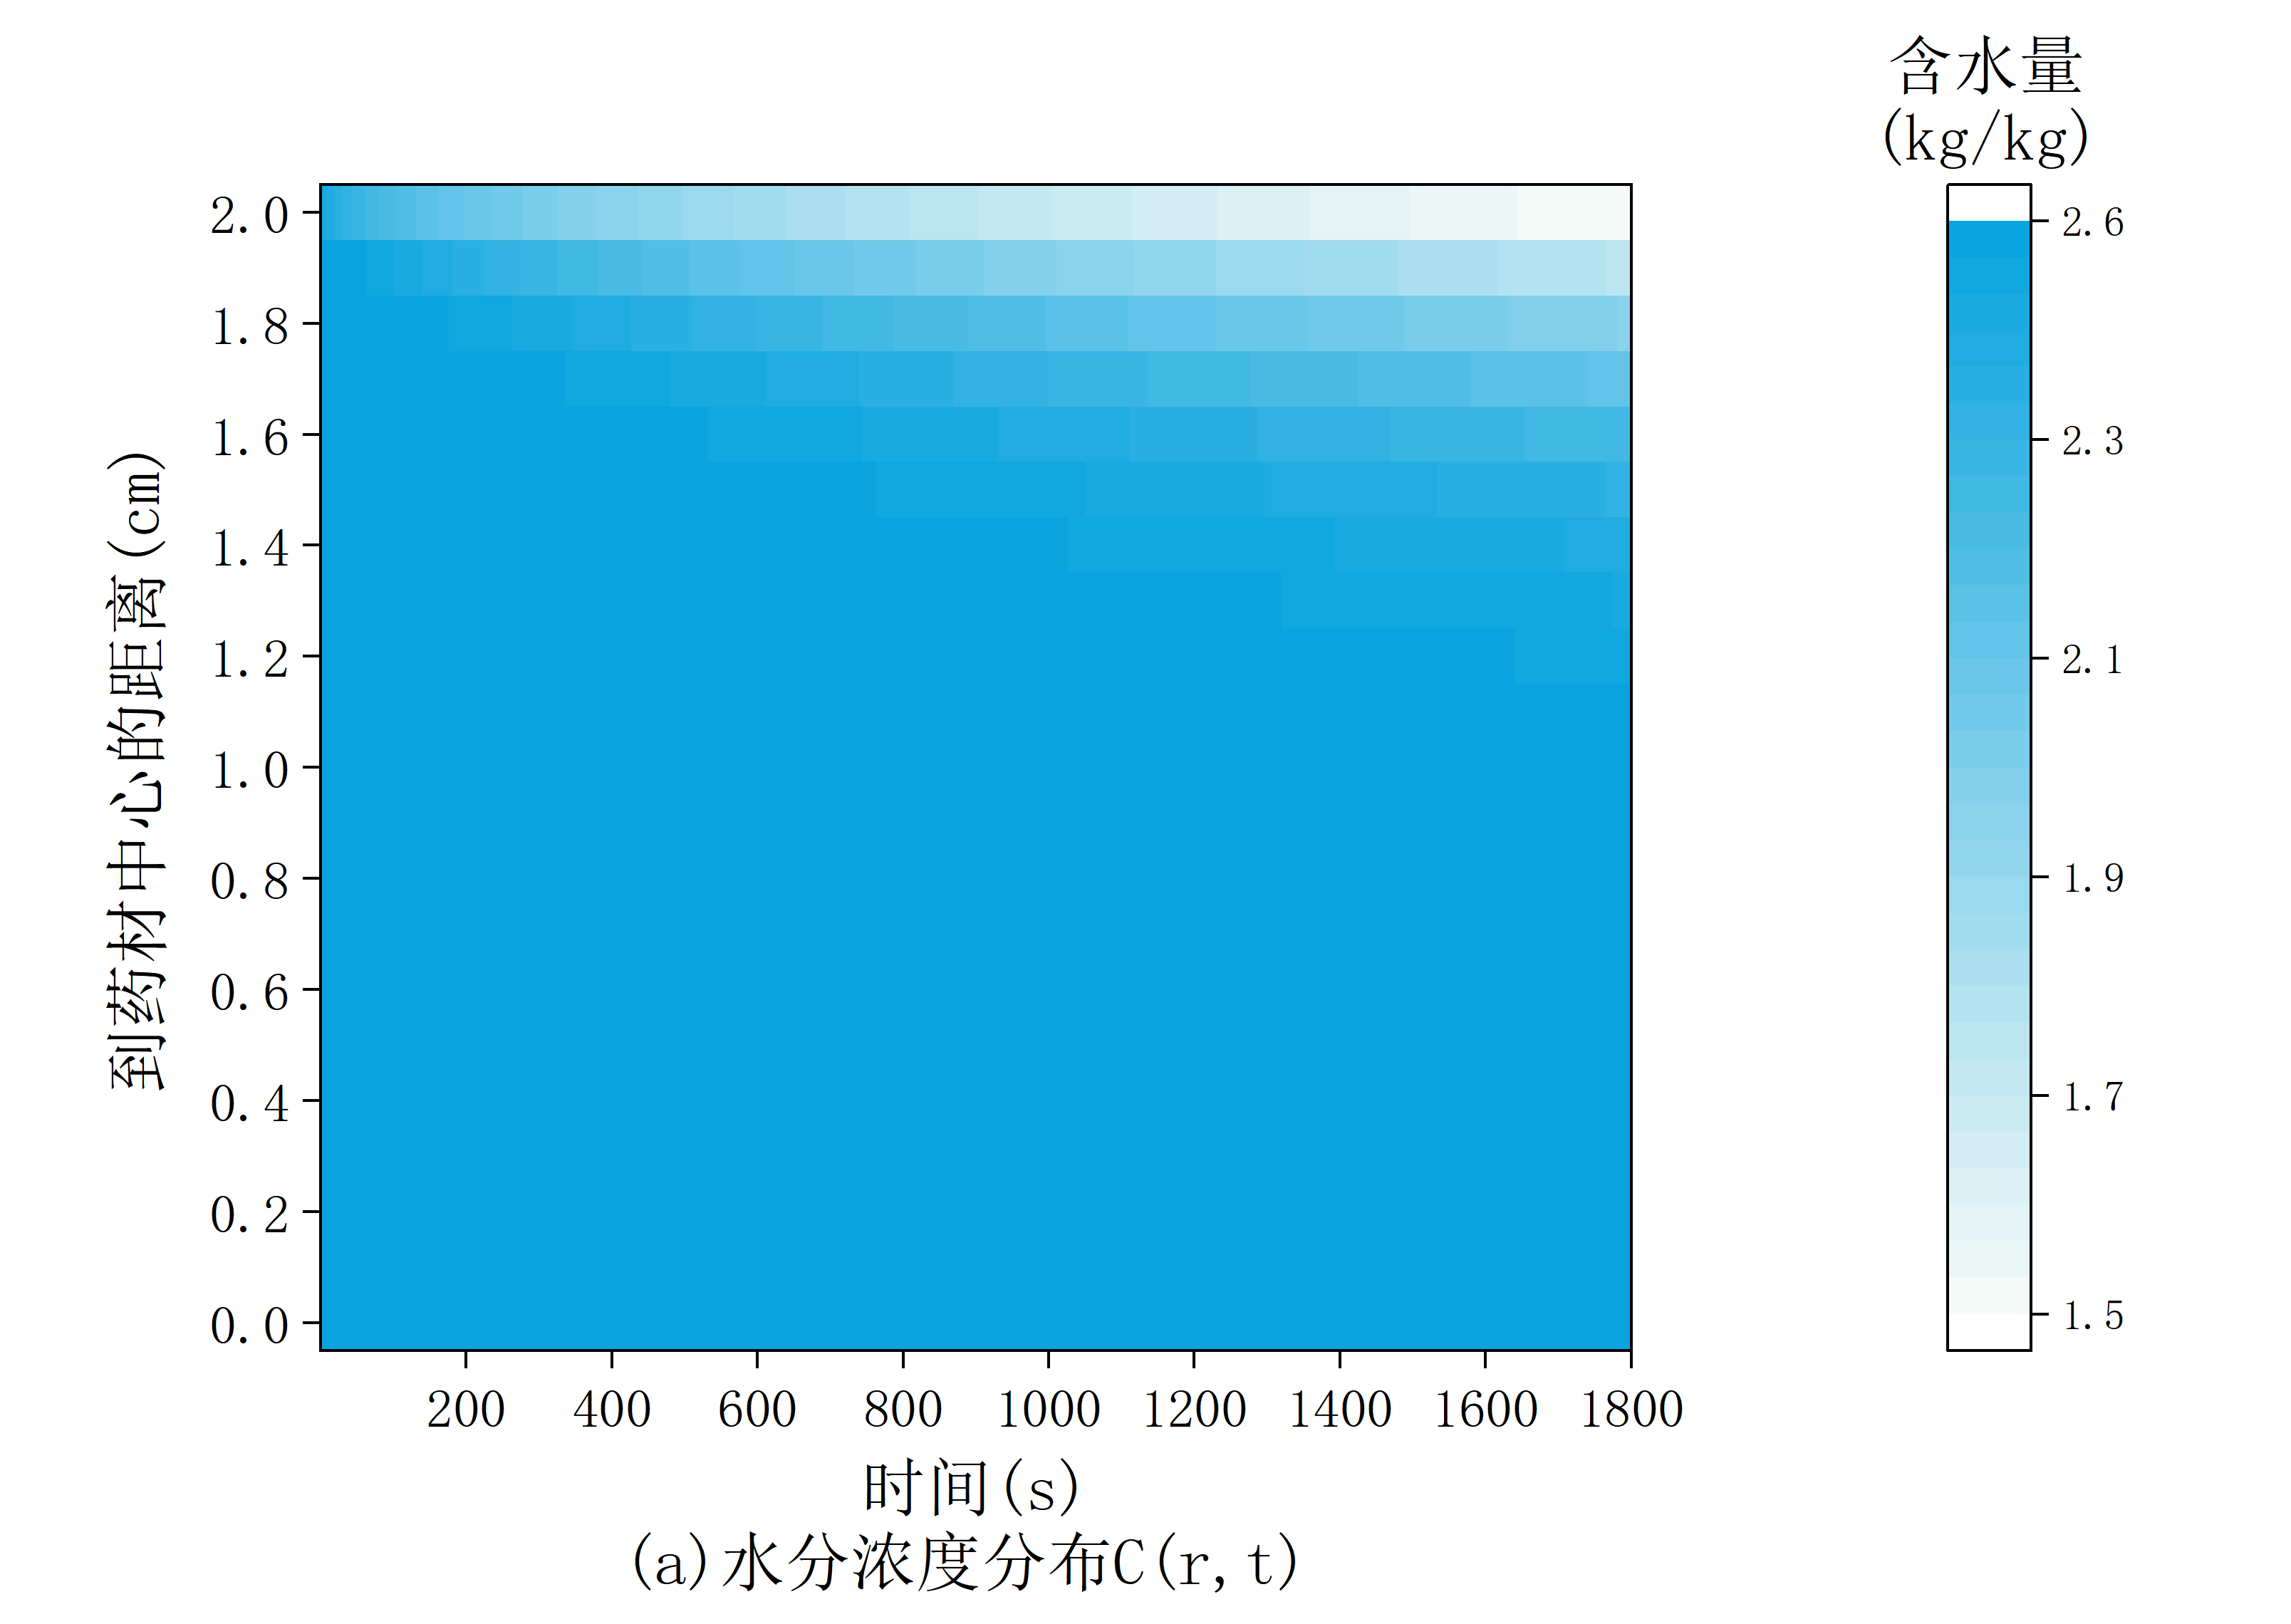
\includegraphics[trim={632.400bp 488.400bp 66.240bp 8.400bp},clip,
      height=0.040695128\unitlength]{图5(a).png}}}
  % (b)径向剖面，保持原比例，与(a)的轴框上下对齐。
  \put(0.514889610,0.010419823){\makebox(0,0)[lb]{%
    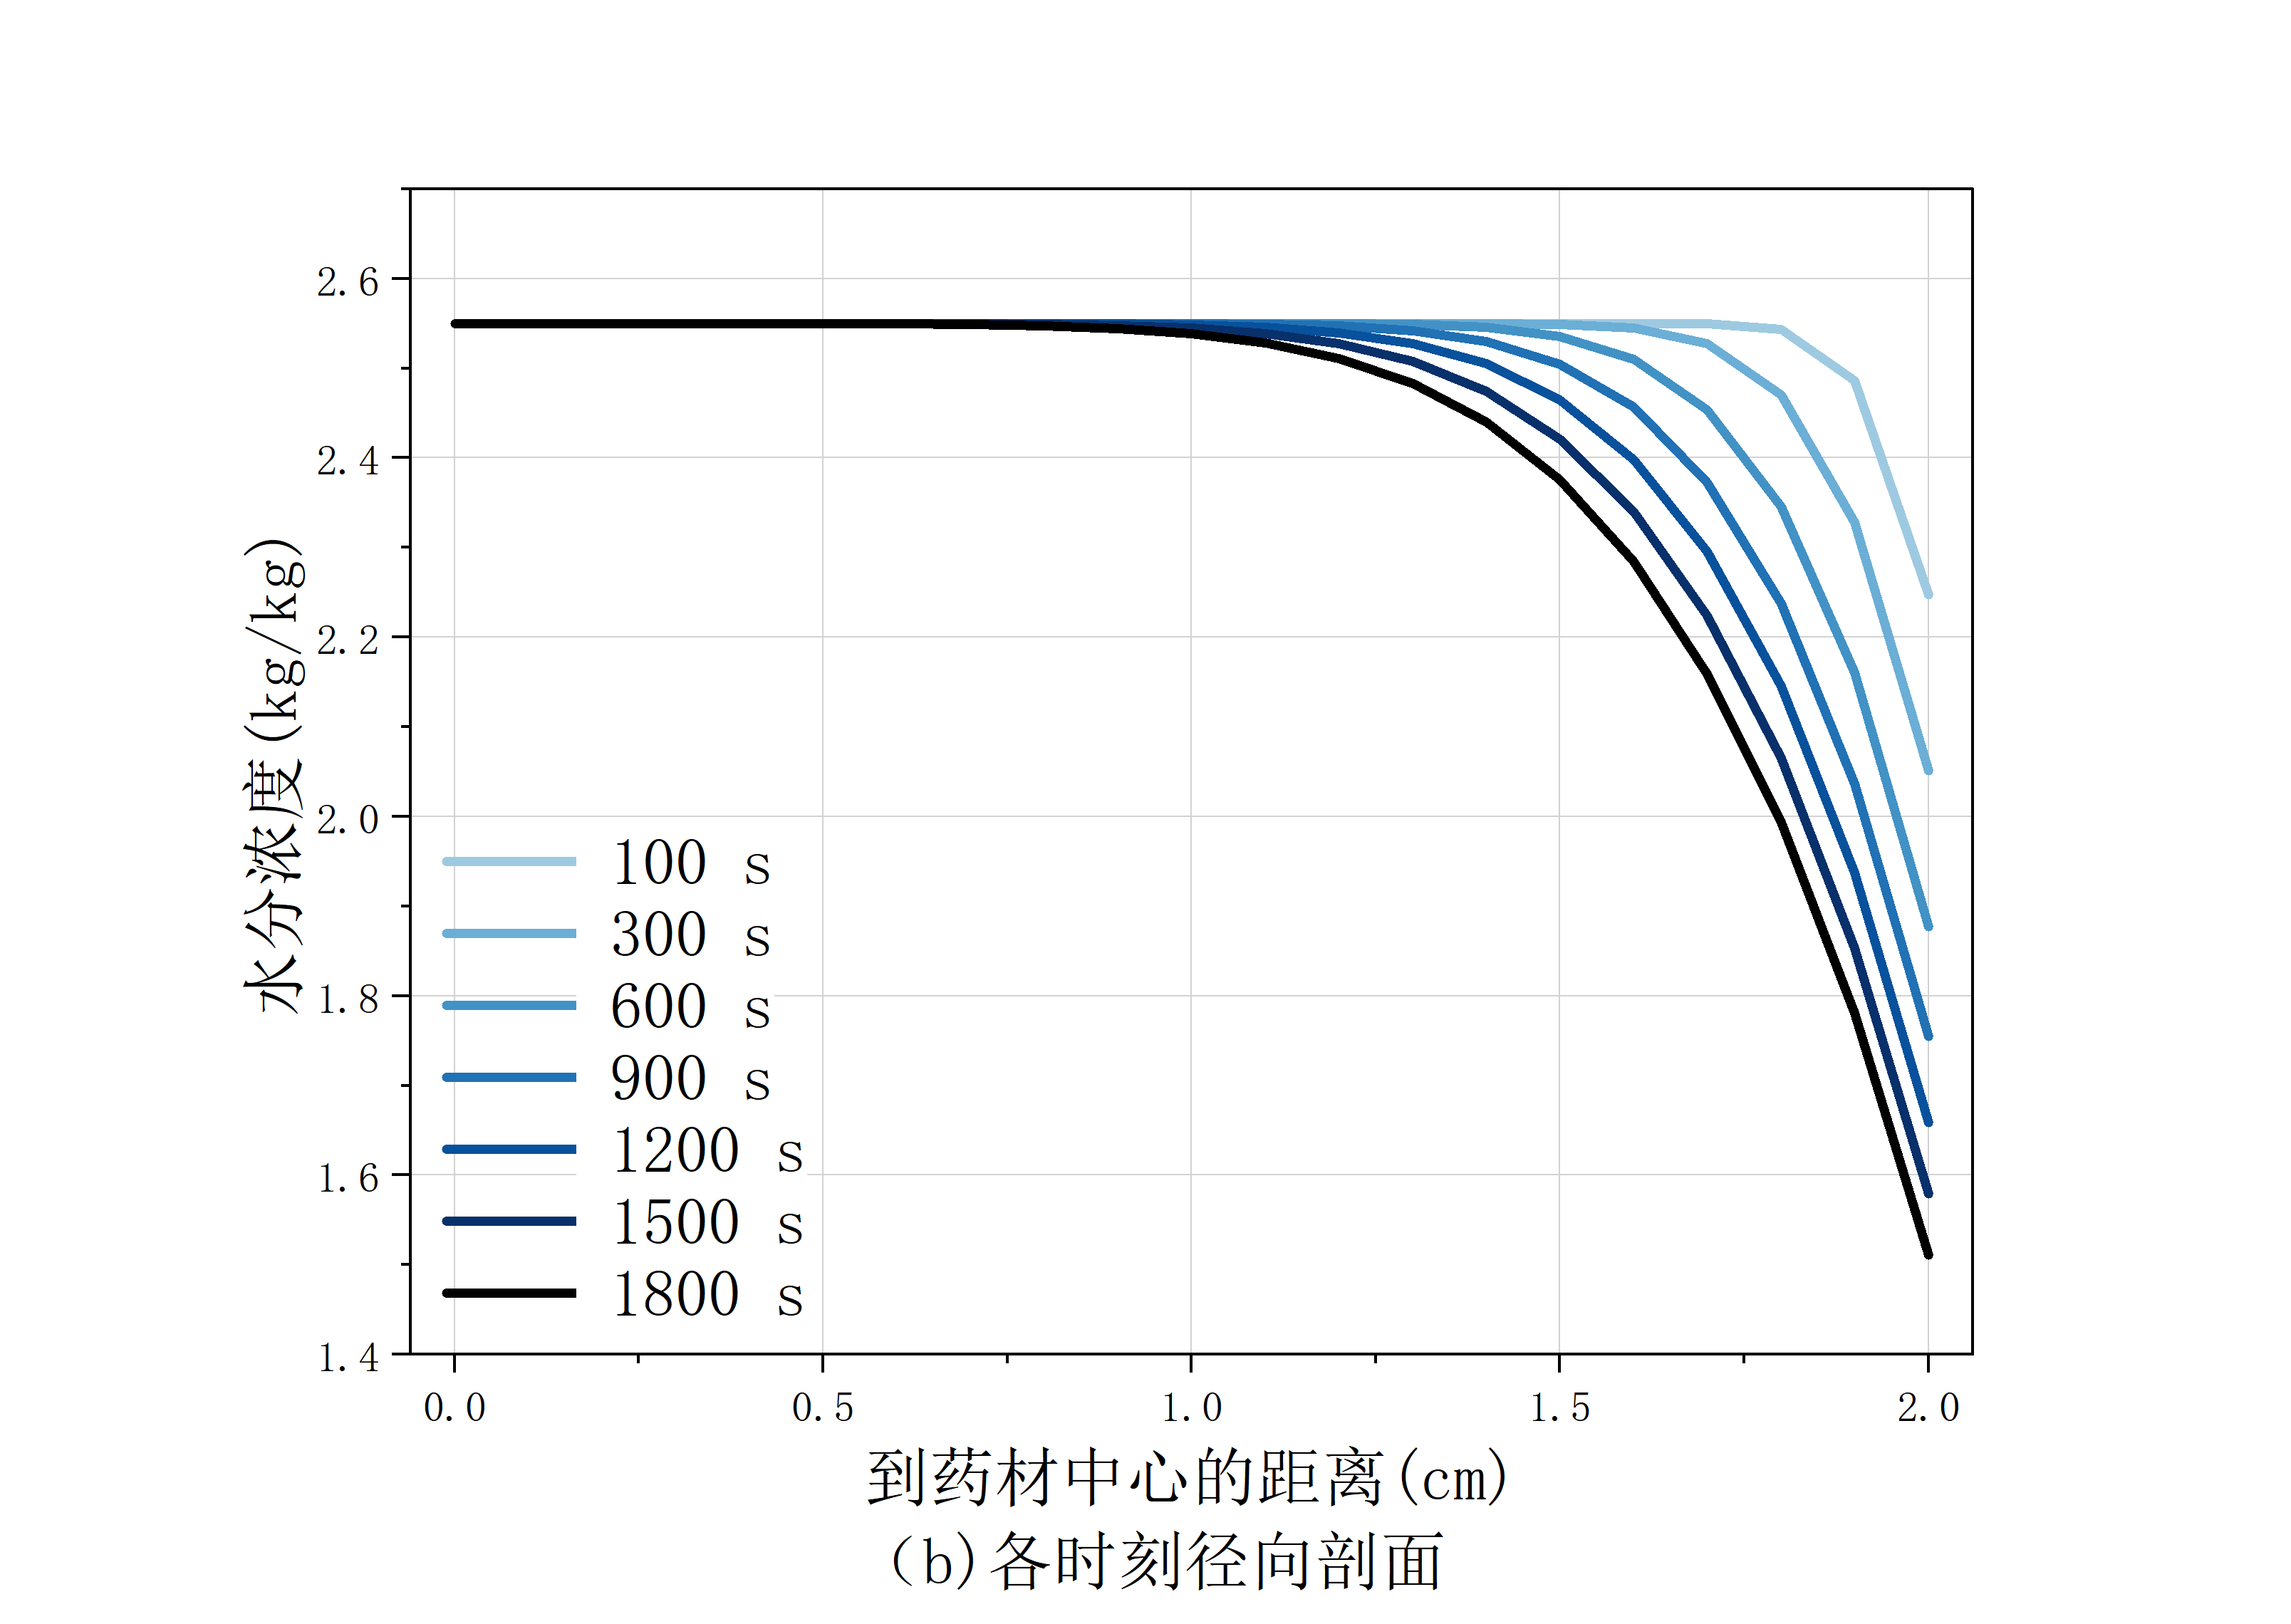
\includegraphics[trim={78.000bp 36.000bp 102.240bp 34.800bp},clip,
      height=0.384900980\unitlength]{图5(b).png}}}
\end{picture}
\caption{问题一水分场及不同时刻的径向含水率剖面}
\label{fig:p1-moisture}
\end{figure}

由式\eqref{eq:p1-biot}，热、质毕渥数分别为$1.3889$和$3.2404$，
两场均存在不可忽略的内部传递阻力，且水分内部扩散相对于表面交换受到的限制更突出。
外层失水使$D(C)$减小、传质毕渥数进一步增大，因此\textbf{表层先失水，内部水分补给滞后}。
毕渥数反映阻力比例，响应先后还取决于传递时间尺度：热扩散率
$\alpha=k/(\rho c_p)\approx1.69\times10^{-7}\ \mathrm{m^2/s}$约为$D(C_0)$的$34.2$倍，
同一径向尺度下热量向内传播更快；结合中心已经升温而含水率基本不变的结果，
可见\textbf{温度变化的影响先深入内部，内部失水响应相对滞后}。


% 此处允许前节浮动图自然排放，避免节首浮动屏障触发换页。
\let\savedSectionFloatBarrier\FloatBarrier
\let\FloatBarrier\relax
\section{问题二模型的建立与求解}
\let\FloatBarrier\savedSectionFloatBarrier
\label{sec:p2}
% 6.1：以附录3及既定显热、固定域假设建立双向变物性耦合模型。
\subsection{模型建立}
\label{sec:p2-model}

问题二沿用问题一的固定圆柱径向模型、守恒关系及显热近似，
以状态相关物性连接温度与含水率，形成双向耦合。
此类通过状态相关物性描述热湿相互作用的思路，已用于生物多孔介质热风干燥建模\cite{porous-drying}。

\subsubsection{状态相关物性与双向反馈关系}

仍以$T(r,t)$和$C(r,t)$为两个待求场量，令$T_K=T+273.15$为绝对温度。
本问物性由局部状态确定：
\begin{equation}
\begin{aligned}
  \rho(C)&=650+128C
    &&\mathrm{kg/m^3},\\
  c_p(C)&=1450+2736\frac{C}{C+1}
    &&\mathrm{J/(kg\,K)},\\
  k(C)&=0.21+0.38\frac{C}{C+1}
    &&\mathrm{W/(m\,K)},\\
  D(C,T_K)&=2.4\times10^{-3}
    \exp\!\left(-\frac{0.45}{C}\right)
    \exp\!\left(-\frac{3850}{T_K}\right)
    &&\mathrm{m^2/s}.
\end{aligned}
\label{eq:p2-properties}
\end{equation}
由式\eqref{eq:p2-properties}知，$C>0$时
$\partial D/\partial T_K>0$、$\partial D/\partial C>0$。
在本题向外排湿条件下，温度升高使水分扩散系数$D$增大，促进水分向表面迁移并增强失水；
失水又使含水率$C$降低，从而减小$D$，抑制后续水分迁移，形成负反馈。
这一促进与抑制关系及含水率对热物性的反馈见图\ref{fig:p2-coupling}。

\begin{figure}[!htbp]
  \centering
  \begin{tikzpicture}[
    box/.style={draw,rounded corners=2pt,fill=black!3,align=center,
      minimum height=1.05cm,text width=2.7cm,inner sep=5pt,font=\small},
    flow/.style={-{Stealth[length=2mm]},semithick},
    every node/.append style={font=\small}
  ]
    \node[box] (temp) at (0,0) {温度升高\\$T\uparrow$};
    \node[box] (diff) at (4.7,0) {水分扩散系数\\$D(C,T_K)$};
    \node[box] (water) at (9.4,0) {含水率\\$C(r,t)$};
    \node[box,text width=4.0cm] (thermal) at (4.7,-2.1)
      {热容量$\rho(C)c_p(C)$\\导热系数$k(C)$};
    \draw[flow] (temp.east) -- node[above]{$+$} node[below]{增大$D$} (diff.west);
    \draw[flow] (diff.east) -- node[above]{$-$} node[below]{促进失水} (water.west);
    \draw[flow] (water.north) to[out=90,in=90,looseness=1.1]
      node[above]{$+$：$C\downarrow$使$D\downarrow$} (diff.north);
    \draw[flow] (water.south) -- (9.4,-2.1)
      -- node[below]{$+$：同向变化} (thermal.east);
    \draw[flow] (thermal.west) -- node[below]{$\pm$：综合热响应} (0,-2.1)
      -- (temp.south);
    \node[align=center,font=\footnotesize] at (4.7,-3.25)
      {$+$表示同向影响，$-$表示反向影响；$D\to C\to D$构成负反馈。\\
       $D\to C$表示整体失水趋势，各位置的局部响应由耦合方程确定。\\
       $\pm$表示热容量与导热能力共同作用，温度变化方向由热方程确定。};
  \end{tikzpicture}
  \caption{问题二温度、含水率与物性之间的反馈关系}
  \label{fig:p2-coupling}
\end{figure}

\subsubsection{非线性热质耦合方程的建立}

沿用问题一的推导，将式\eqref{eq:p1-heat}、式\eqref{eq:p1-mass}中的物性
替换为式\eqref{eq:p2-properties}，将变系数$k(C)$和$D(C,T_K)$保留在散度内部，得到
\begin{equation}
\left\{
\begin{aligned}
  \rho(C)c_p(C)\frac{\partial T}{\partial t}
    &=\frac{1}{r}\frac{\partial}{\partial r}
      \left[rk(C)\frac{\partial T}{\partial r}\right],\\
  \frac{\partial C}{\partial t}
    &=\frac{1}{r}\frac{\partial}{\partial r}
      \left[rD(C,T_K)\frac{\partial C}{\partial r}\right],
\end{aligned}
\right.
\qquad 0<r<R_0,\quad t>0.
\label{eq:p2-coupled-pde}
\end{equation}
其中$\rho(C)$仍用于有效热容量计算；水分方程沿用问题一的干基变量及干骨架假设。

\subsubsection{初边条件的沿用与物性更新}

初值、中心对称条件及环境插值与延拓分别沿用式\eqref{eq:p1-initial}、
式\eqref{eq:p1-center}和式\eqref{eq:p1-environment}。
表面边界沿用式\eqref{eq:p1-boundary-heat}、式\eqref{eq:p1-boundary-mass}，
其中$k$、$D$分别更新为当前表面状态对应的$k(C_s)$、$D(C_s,T_s+273.15)$，
$h$、$h_m$及表面值定义不变。
全过程从原始初态$t=0$起统一采用附录3物性。

% 6.2：与code/p23.py的双场中点Picard迭代一致；沿用既有生产结果，未重算PDE。
\subsection{模型求解}
\label{sec:p2-solution}

空间离散沿用问题一的有限体积法，时间推进沿用式\eqref{eq:p1-time}。
通过双场Picard迭代，在每个时间步内同步确定两场及其物性。

\subsubsection{中点物性下的双场同步迭代}

设$\Delta t_n=t^{n+1}-t^n$，已知第$n$层的$\boldsymbol T^n$、$\boldsymbol C^n$。
以旧层解作为新层初始估计，即
$\boldsymbol T^{n+1,(0)}=\boldsymbol T^n$、
$\boldsymbol C^{n+1,(0)}=\boldsymbol C^n$。
第$\ell$轮由当前估计构造同一时间中点的状态
\begin{equation}
  \widetilde T_i^{(\ell)}
    =\frac{T_i^n+T_i^{n+1,(\ell)}}{2},\qquad
  \widetilde C_i^{(\ell)}
    =\frac{C_i^n+C_i^{n+1,(\ell)}}{2}.
  \label{eq:p2-midpoint}
\end{equation}
将其代入式\eqref{eq:p2-properties}，计算节点导热系数
$k_i^{(\ell)}=k(\widetilde C_i^{(\ell)})$和扩散系数
$D_i^{(\ell)}=D(\widetilde C_i^{(\ell)},\widetilde T_i^{(\ell)}+273.15)$。
按式\eqref{eq:p1-fvm-coefficients}取相邻节点物性的算术平均，
分别得到温度场、水分场的面导通系数$G_{T,i+1/2}^{(\ell)}$、
$G_{C,i+1/2}^{(\ell)}$；两场对应的时间项系数为
\begin{equation}
  m_{T,i}^{(\ell)}
    =\frac{\rho(\widetilde C_i^{(\ell)})
       c_p(\widetilde C_i^{(\ell)})V_i}{\Delta t_n},
  \qquad
  m_{C,i}=\frac{V_i}{\Delta t_n}.
  \label{eq:p2-time-coefficients}
\end{equation}

将上述系数及$B_T=R_0h$、$B_C=R_0h_m$分别代入式\eqref{eq:p1-linear-system}，
组装两场的三对角系统；本轮新、旧层通量使用同一组固定的面系数，
步首、步末环境值按式\eqref{eq:p1-surface-row}加权进入右端。

每轮以同一组中点物性分别求解两场，两场解出后同步更新式\eqref{eq:p2-midpoint}。
仅当两场同时满足式\eqref{eq:picard-tolerance}时才接受时间步，
迭代上限为30轮，超限则报告未收敛。
全程仅最初两步取$\theta=1$作隐式启动，其余取$\theta=1/2$，
物性均按中点状态计算。

\subsubsection{数值实现与计算结果}

线性求解器沿用第\ref{sec:p1-solution}节的设置。
采用同一882节点网格及外侧$0.5\ \mathrm{mm}$加密区域，
前$60\ \mathrm{s}$取$\Delta t_n=0.03125\ \mathrm{s}$，
此后取$0.25\ \mathrm{s}$推进至$10800\ \mathrm{s}$。
每隔$1\ \mathrm{s}$在$r=0,0.1,\ldots,2.0\ \mathrm{cm}$处提取两场结果，
以四位小数保存至\texttt{result2.xlsx}；题目指定的结果列于表\ref{tab:p2T}、表\ref{tab:p2C}。

\begin{table}[!htbp]
  \centering
  \caption{3小时内药材的温度（单位：$^{\circ}\mathrm{C}$）}
  \label{tab:p2T}
  \begin{tabularx}{\textwidth}{@{}YYYYYY@{}}
    \toprule
    \multirow{2}{*}{时间/$\mathrm{h}$}&\multicolumn{5}{c}{到药材中心的距离/$\mathrm{cm}$}\\
    \cmidrule(lr){2-6}
    &0&0.5&1&1.5&2\\
    \midrule
    0.5 &32.1892&32.3821&32.9659&33.9608&35.4130\\
    1.0 &40.3816&40.5536&41.0605&41.8782&42.9976\\
    1.5 &45.8468&45.9348&46.1930&46.6051&47.1401\\
    2.0 &48.4502&48.4881&48.5984&48.7736&49.0033\\
    2.5 &49.4670&49.4792&49.5136&49.5653&49.6609\\
    3.0 &49.8495&49.8553&49.8746&49.9101&49.9664\\
    \bottomrule
  \end{tabularx}
\end{table}

\begin{table}[!htbp]
  \centering
  \caption{3小时内药材的水分浓度（单位：$\mathrm{kg/kg}$）}
  \label{tab:p2C}
  \begin{tabularx}{\textwidth}{@{}YYYYYY@{}}
    \toprule
    \multirow{2}{*}{时间/$\mathrm{h}$}&\multicolumn{5}{c}{到药材中心的距离/$\mathrm{cm}$}\\
    \cmidrule(lr){2-6}
    &0&0.5&1&1.5&2\\
    \midrule
    0.5 &2.5499&2.5489&2.5256&2.3257&1.6486\\
    1.0 &2.5257&2.4948&2.3578&2.0230&1.4711\\
    1.5 &2.3861&2.3256&2.1344&1.8020&1.3476\\
    2.0 &2.1709&2.1084&1.9236&1.6259&1.2311\\
    2.5 &1.9566&1.9006&1.7360&1.4720&1.1166\\
    3.0 &1.7662&1.7165&1.5702&1.3333&1.0081\\
    \bottomrule
  \end{tabularx}
\end{table}

% 6.3：依据表3、表4及同源的已保存数值场分析结果；图6使用用户提供的两张PNG。
\subsection{结果分析}
\label{sec:p2-analysis}

表\ref{tab:p2T}、表\ref{tab:p2C}及图\ref{fig:p2-evolution}展示前$3\ \mathrm{h}$的温湿变化，
图中药材曲线分别对应中心、$r=1\ \mathrm{cm}$处及表面，与表格采用同一数值解。

\subsubsection{温度逐渐趋于均匀}

图\ref{fig:p2-evolution}(a)显示，\textbf{表面先升温，中心响应滞后，随后各位置温度逐渐靠拢。}
表面与中心的温差由$0.5\ \mathrm{h}$时的$3.2238\tempunit$
缩小至$3\ \mathrm{h}$时的$0.1169\tempunit$，
此时表列各位置的温度为$49.8495$--$49.9664\tempunit$，已接近烘房温度。

\begin{figure}[!htbp]
\centering
% 保持原图6的0.98\textwidth宽度及264.543625/634.2825高宽比。
% 以相同范围裁去两张PNG的白边，完整保留标题、图例、单位及最右侧刻度。
% trim按源PNG的300 dpi换算；仅指定高度以保持原比例，轴框宽度及水平位置沿用原图。
\setlength{\unitlength}{0.98\textwidth}
\begin{picture}(1,0.417075396)
  \put(0.004323459,0.014316401){\makebox(0,0)[lb]{%
    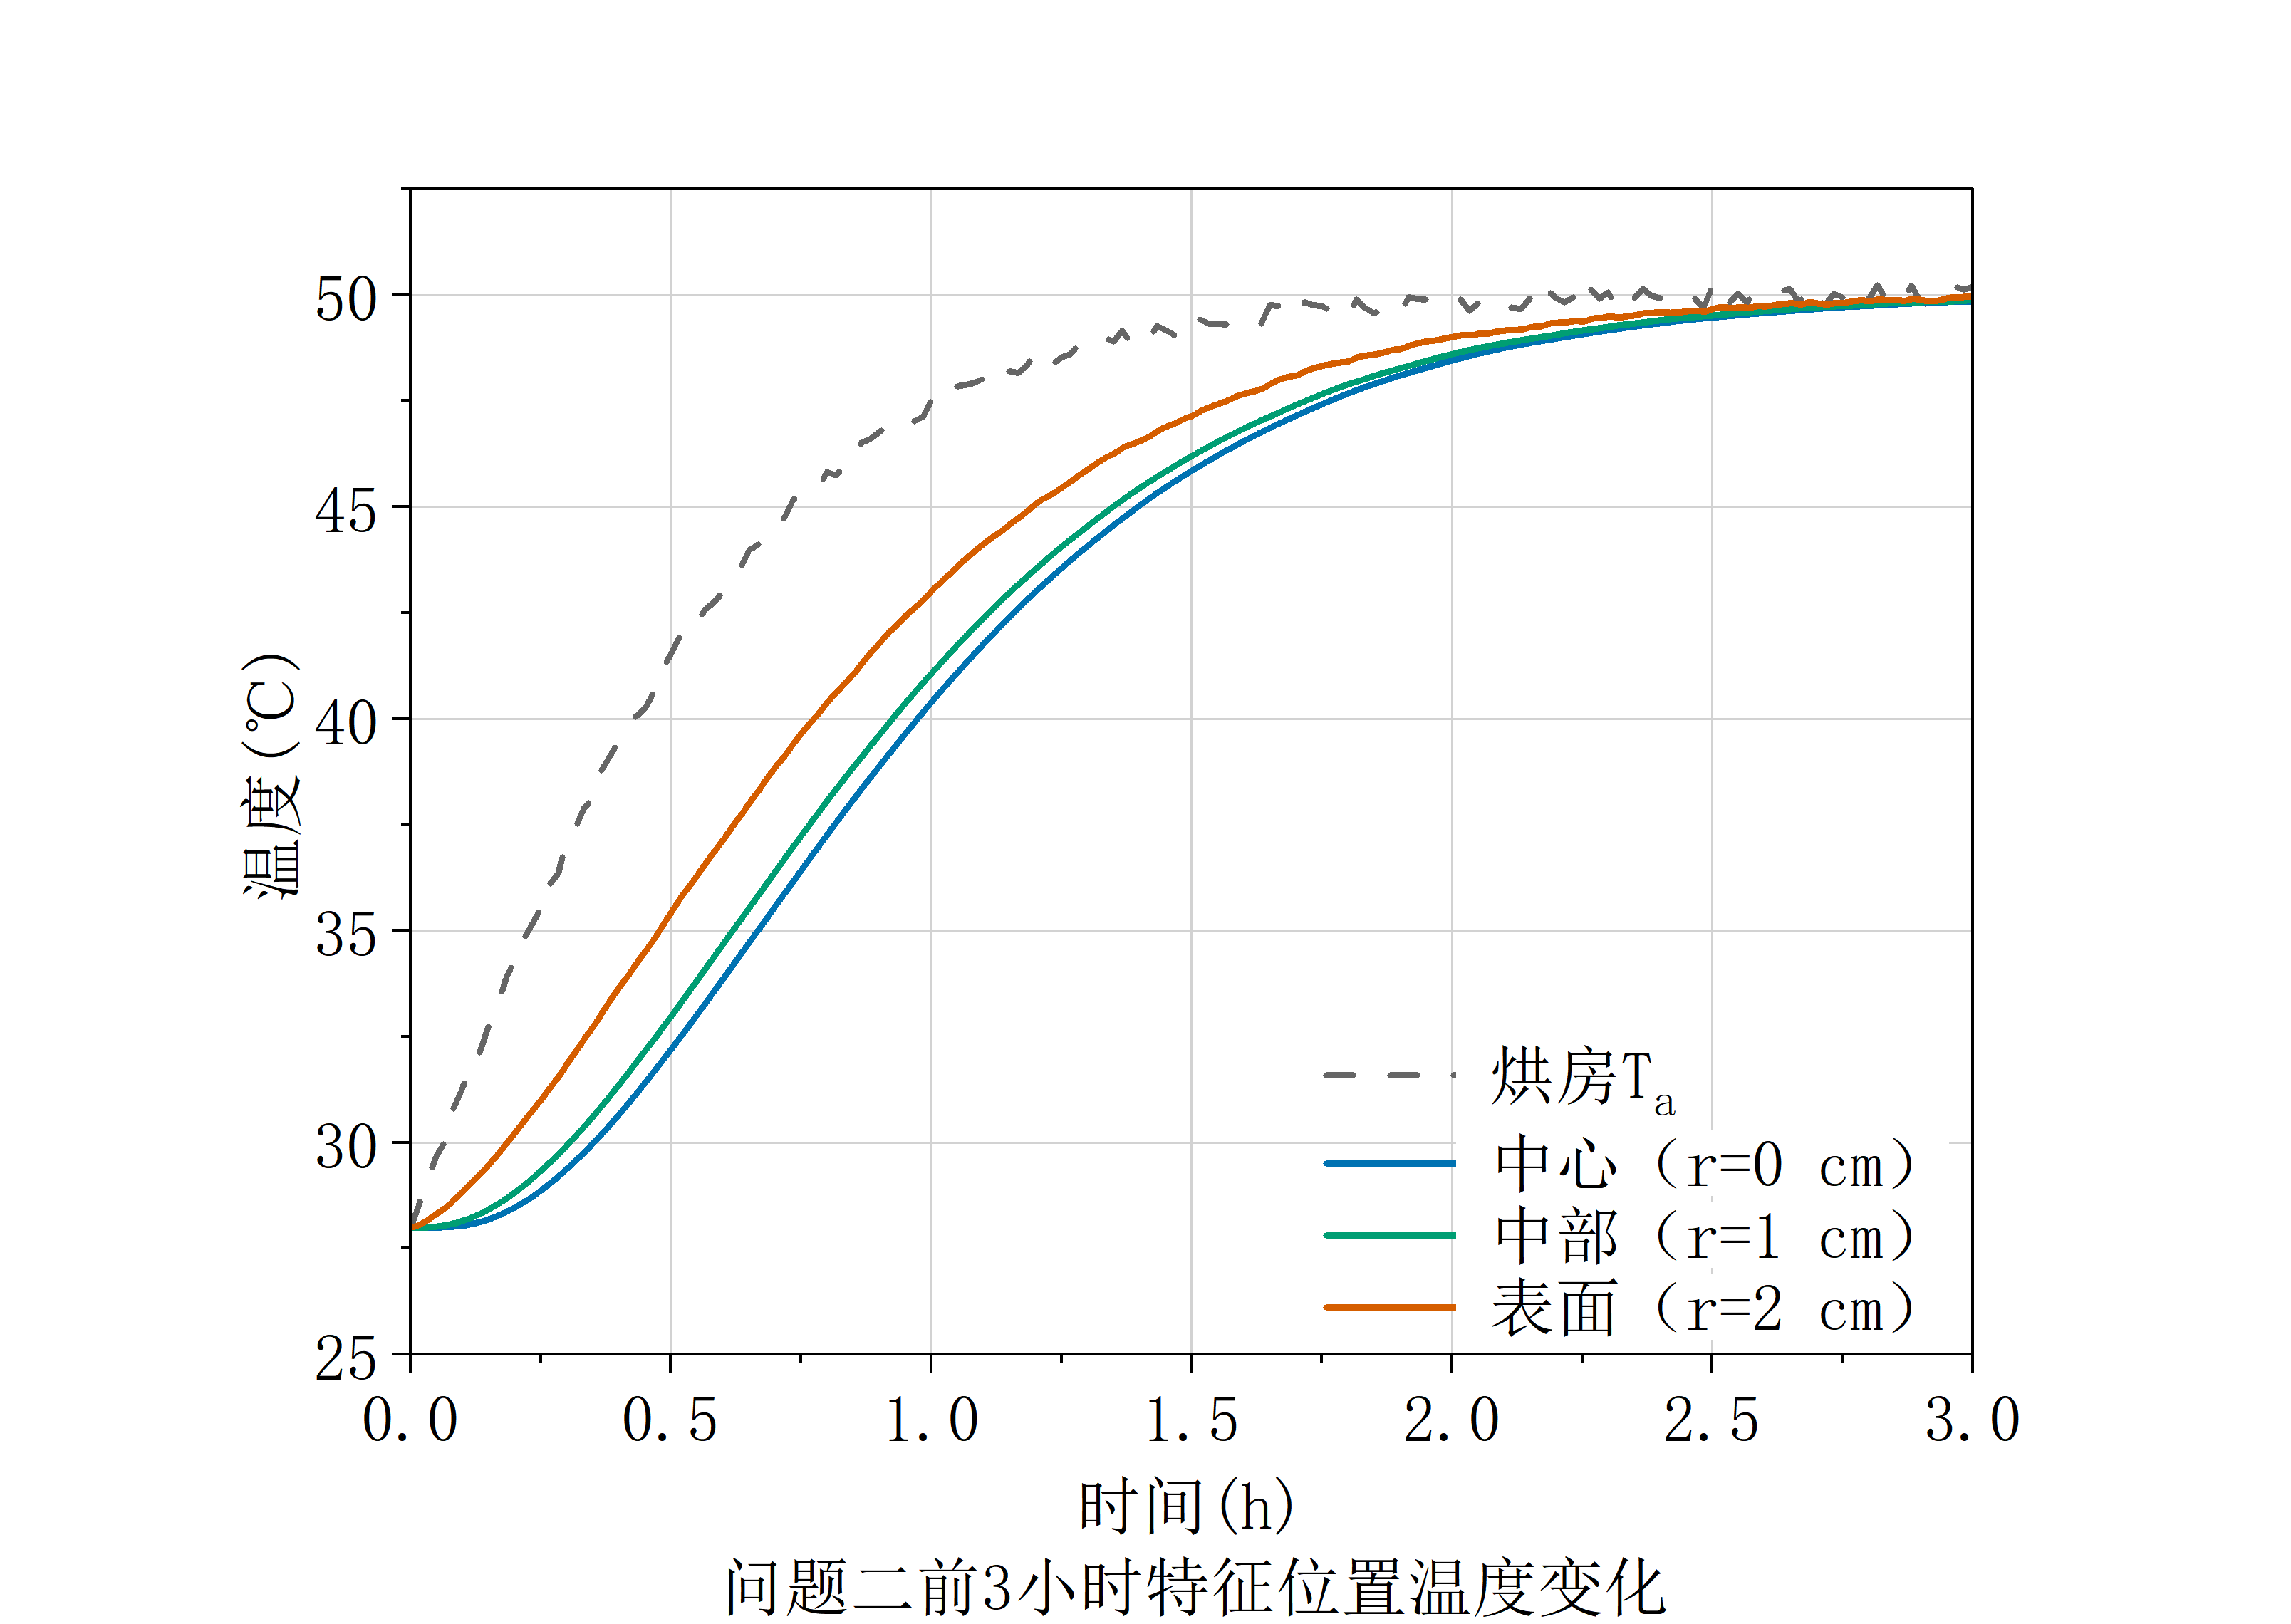
\includegraphics[trim={66.000bp 26.400bp 87.840bp 32.400bp},clip,
      height=0.385911668\unitlength]{图7(a).png}}}
  \put(0.503372671,0.014316401){\makebox(0,0)[lb]{%
    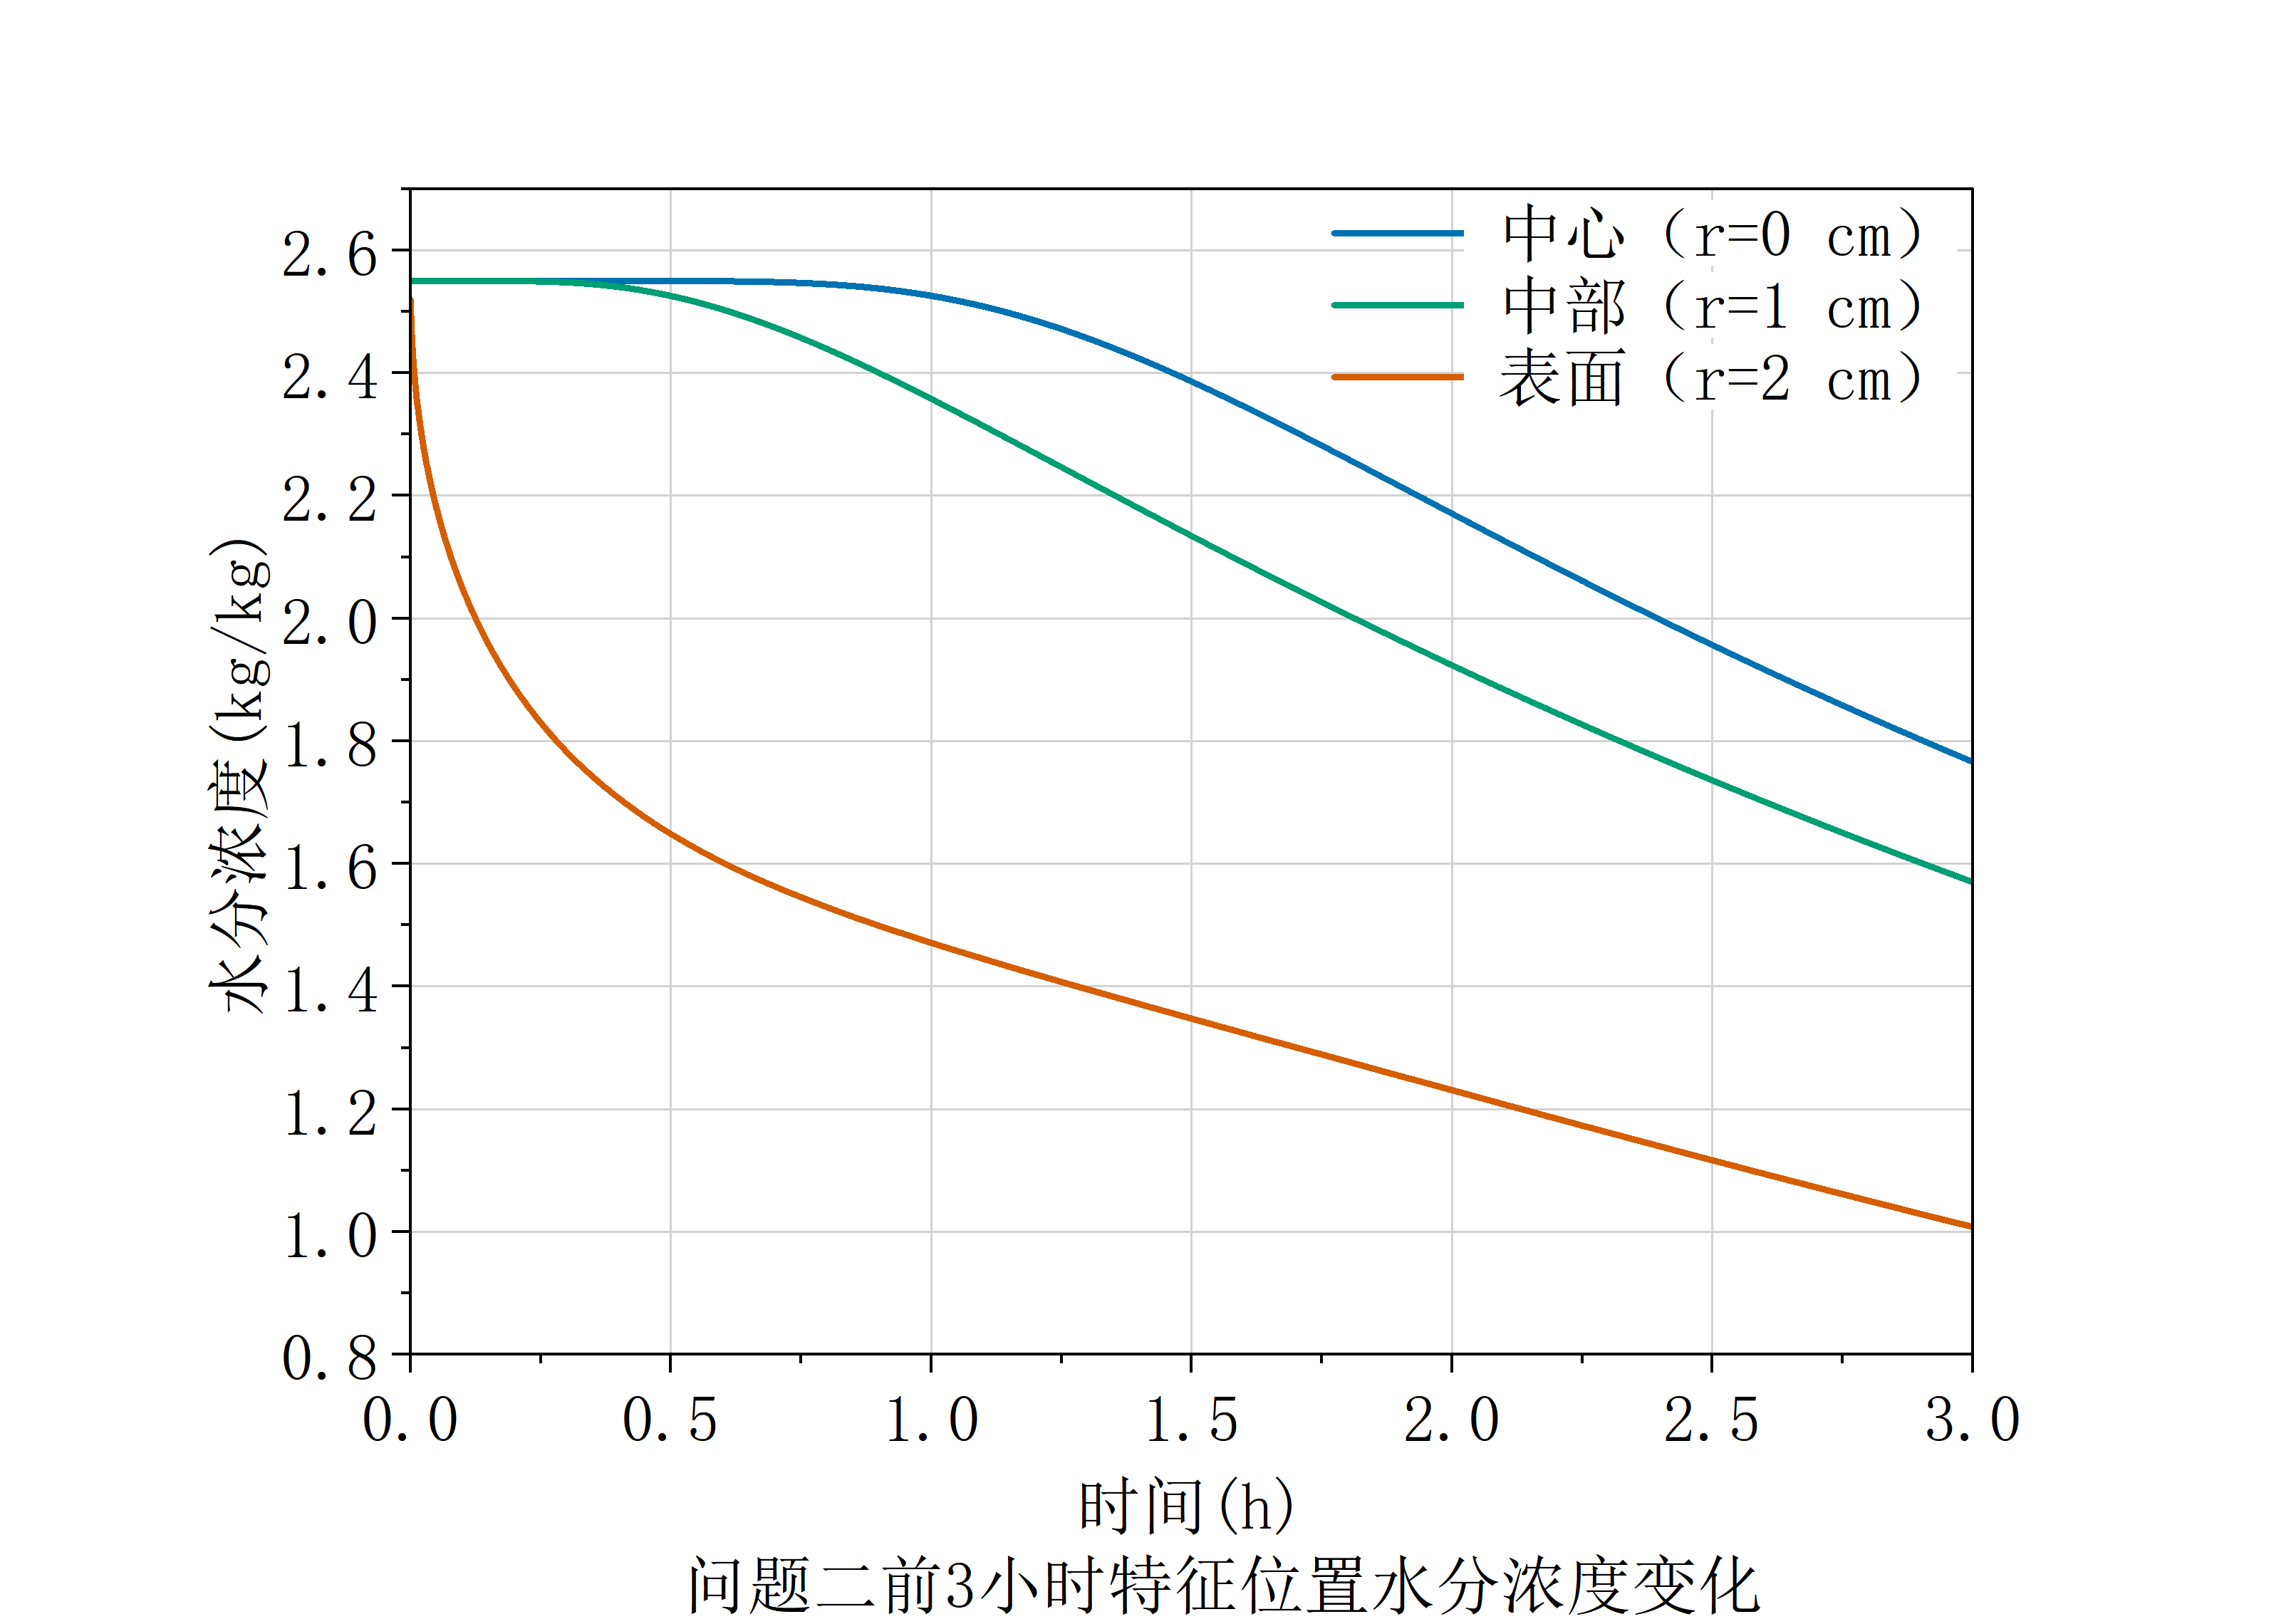
\includegraphics[trim={66.000bp 26.400bp 87.840bp 32.400bp},clip,
      height=0.385911668\unitlength]{图7(b).png}}}
\end{picture}
\caption{问题二前3 h特征位置的温度和含水率变化}
\label{fig:p2-evolution}
\end{figure}

\subsubsection{水分滞后与变物性作用}

图\ref{fig:p2-evolution}(b)显示，表面含水率初期迅速下降，中心随后才明显失水。
中心与表面的差值由$0.5\ \mathrm{h}$时的$0.9013\cunit$
增至$1\ \mathrm{h}$时的$1.0546\cunit$，
再降至$3\ \mathrm{h}$时的$0.7581\cunit$。
这一先增后减的变化反映了表面先失水、内部随后参与的过程，
但本时段末仍保留明显的内湿外干分布。

$3\ \mathrm{h}$时中心和表面含水率分别为$1.7662\cunit$、$1.0081\cunit$。
将对应温湿状态代入式\eqref{eq:p2-properties}，所得扩散系数约为
$1.24\times10^{-8}\ \mathrm{m^2/s}$和
$1.03\times10^{-8}\ \mathrm{m^2/s}$。
虽然表面温度略高，较干外层的扩散能力仍偏低，说明在这两个位置的比较中，
较低含水率的影响超过了微小温差对扩散的促进作用。
\textbf{因此，温度趋于均匀与水分脱除并不同步，局部含水率仍通过物性影响后续水分迁移。}


\section{问题三模型的建立与求解}
\label{sec:p3}
% 7.1：沿用问题二的全过程模型，新增全域达标判据与未知终止时间。
\subsection{模型建立}
\label{sec:p3-model}

问题三在问题二模型上增加全域含水率约束，
要求各处均低于$0.15\cunit$，由此确定未知的临界烘干时间。

\subsubsection{全过程模型的沿用与延续}

沿用第\ref{sec:p2-model}节的全过程模型，以及式\eqref{eq:p1-environment}的插值和前文规定的恒定环境延拓，
将问题二在$3\ \mathrm{h}$时的两场状态继续向后推进，
总时长仍从原始初态$t=0$起算。

\subsubsection{全域达标约束与临界时间}

令$C_*=0.15\cunit$。全域达标要求每个径向位置均满足$C(r,t)<C_*$，
等价于$C_{\max}(t)<C_*$，其中全域最大含水率及临界时间定义为
\begin{align}
  C_{\max}(t)&=\max_{0\le r\le R_0}C(r,t),
  \label{eq:p3-maximum}\\
  t_*&=\inf\left\{t\ge0:\ C_{\max}(t)<C_*\right\}.
  \label{eq:p3-endpoint}
\end{align}
当$C_{\max}(t)$连续向下穿越阈值时，临界处$C_{\max}(t_*)=C_*$，
其后才严格达标；判断须基于未舍入的场量。
烘干结束由含水率最高的位置控制，表面或截面平均含水率不能替代全域判据。
中心能否代表全域最大值，须在求解中逐步核验。

% 7.2：沿用既有生产解；全域控制位置核验及事件定位与code/p23.py一致。
\subsection{模型求解}
\label{sec:p3-solution}

\subsubsection{时间推进与临界时刻定位}

前$3\ \mathrm{h}$沿用第\ref{sec:p2-solution}节的数值设置，
此后取$\Delta t_n=1\ \mathrm{s}$，网格、双场迭代与时间格式不变，
全程仍仅最初两步作隐式启动。

每步收敛后，在全部计算节点上求
$C_{\max}^{n}=\max_{0\le i\le N}C_i^{n}$，
并与中心含水率比较。
全过程核验表明，二者之差始终不超过$10^{-12}\cunit$，
故本次计算中可用中心含水率定位全域达标时刻。
当首次出现$C_{\max}^{n}\ge C_*>C_{\max}^{n+1}$时，认为在该区间内水分浓度持续减小，
临界时刻位于$[t^n,t^{n+1})$内。
对该步的未舍入结果作线性插值，得到
\begin{equation}
\begin{gathered}
  \lambda=\frac{C_{\max}^{n}-C_*}
                 {C_{\max}^{n}-C_{\max}^{n+1}},
  \qquad t_*\approx t^n+\lambda\Delta t_n,\\
  \boldsymbol C(t_*)\approx
    (1-\lambda)\boldsymbol C^n+\lambda\boldsymbol C^{n+1}.
\end{gathered}
\label{eq:p3-event-interpolation}
\end{equation}
该式同时给出临界时刻及径向含水率分布，规定的$60\ \mathrm{s}$间隔仅用于结果采样。

\subsubsection{烘干时长与计算结果}

计算得到，在前述环境延拓条件下，临界烘干时间为
\begin{equation*}
  \boxed{t_*\approx57.4721\ \mathrm{h}}.
\end{equation*}
每隔$6\ \mathrm{h}$提取$r=0,0.5,1,1.5,2\ \mathrm{cm}$处的含水率，
并由式\eqref{eq:p3-event-interpolation}补充临界时刻的分布，结果见表\ref{tab:p3C}。

\begin{table}[!htbp]
  \centering
  \caption{药材烘干过程的水分浓度（单位：$\mathrm{kg/kg}$）}
  \label{tab:p3C}
  \begin{tabularx}{\textwidth}{@{}C{0.22\textwidth}YYYYY@{}}
    \toprule
    \multirow{2}{*}{时间/$\mathrm{h}$}&\multicolumn{5}{c}{到药材中心的距离/$\mathrm{cm}$}\\
    \cmidrule(lr){2-6}
    &0&0.5&1&1.5&2\\
    \midrule
    6  &1.0170&0.9881&0.9015&0.7550&0.5328\\
    12 &0.4561&0.4432&0.4031&0.3297&0.1642\\
    18 &0.2988&0.2915&0.2687&0.2253&0.0845\\
    24 &0.2378&0.2327&0.2167&0.1855&0.0665\\
    30 &0.2058&0.2018&0.1892&0.1641&0.0598\\
    36 &0.1859&0.1825&0.1718&0.1504&0.0566\\
    42 &0.1721&0.1691&0.1597&0.1407&0.0549\\
    48 &0.1618&0.1592&0.1507&0.1334&0.0537\\
    54 &0.1539&0.1514&0.1436&0.1277&0.0530\\
    \mbox{\textbf{57.4721（结束）}}
       &\textbf{0.1500}&\textbf{0.1477}&\textbf{0.1402}&\textbf{0.1249}&\textbf{0.0527}\\
    \bottomrule
  \end{tabularx}
\end{table}

表末行为$C_{\max}=C_*$的临界状态；继续推进至其后的首个整分钟\textbf{$206940\ \mathrm{s}$}，
此时未舍入的$C_{\max}<C_*$。
全程每隔$60\ \mathrm{s}$、径向每隔$0.1\ \mathrm{cm}$采样，以四位小数写入\texttt{result3.xlsx}。

% 7.3：依据表5及同源的60 s采样场分析长期干燥特征；图7使用用户提供的两张PNG。
\subsection{结果分析}
\label{sec:p3-analysis}

\subsubsection{末期减速及扩散能力衰减}

由表\ref{tab:p3C}估算，中心含水率在$6$--$12\ \mathrm{h}$内下降$0.5609\cunit$，
而在$48$--$54\ \mathrm{h}$内仅下降$0.0079\cunit$。
\textbf{两个时间窗等长，前者的平均下降速率约为后者的70倍} ，
与图\ref{fig:p3-drying}(a)后期曲线趋平的现象一致。

$6\ \mathrm{h}$后温度已基本稳定在$50\tempunit$附近。
将未舍入状态代入式\eqref{eq:p2-properties}，表面扩散系数由$6\ \mathrm{h}$时约
$6.91\times10^{-9}\ \mathrm{m^2/s}$降至$54\ \mathrm{h}$时约
$3.29\times10^{-12}\ \mathrm{m^2/s}$。
低含水率外层的扩散能力减弱，连同表面交换驱动力的下降，使持续脱水受限，
因而\textbf{不能按前期速率线性外推终点}。

\begin{figure}[!htbp]
\centering
% 保持原图7的0.98\textwidth宽度及264.5905/633.317547高宽比。
% 统一裁去两张PNG的白边，完整保留上方结束时间与右侧烘干判据。
% trim按源PNG的300 dpi换算；仅指定宽度以保持原比例，两图的轴框上下对齐。
\setlength{\unitlength}{0.98\textwidth}
\begin{picture}(1,0.417784887)
  \put(0,0.031758297){\makebox(0,0)[lb]{%
    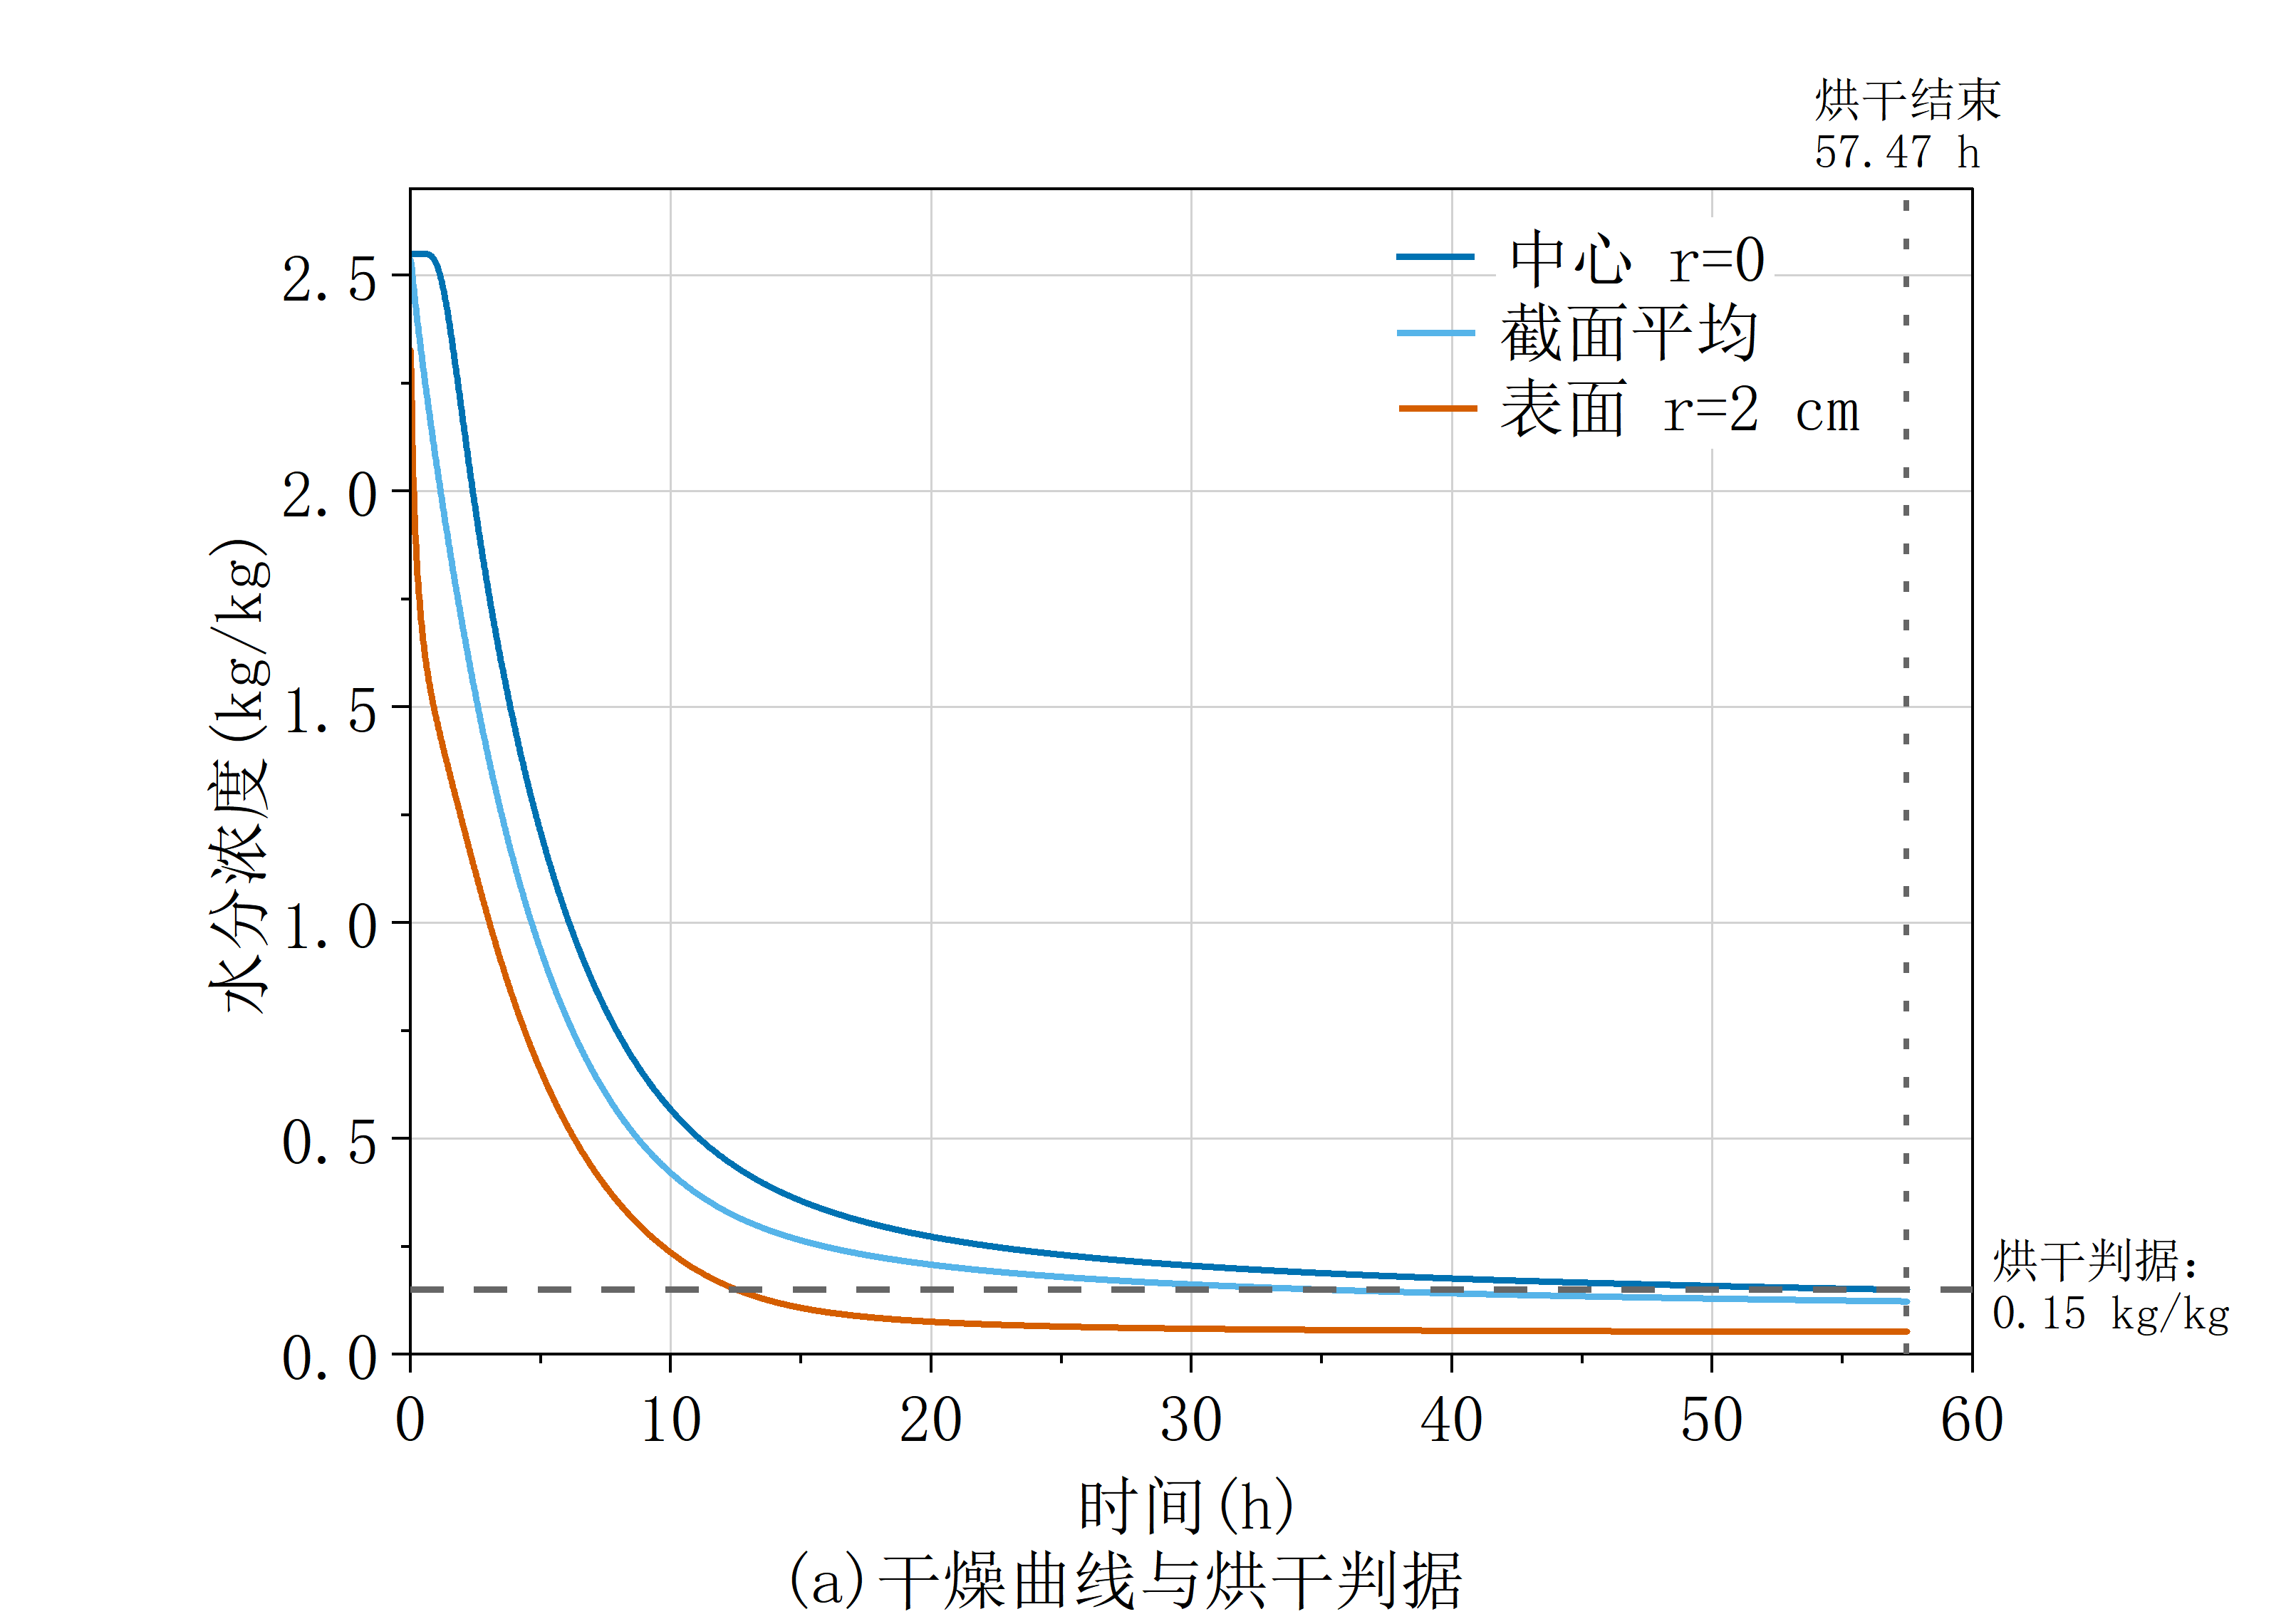
\includegraphics[trim={66.000bp 26.400bp 17.040bp 22.800bp},clip,
      width=0.49\unitlength]{图8(a).png}}}
  \put(0.51,0.031758297){\makebox(0,0)[lb]{%
    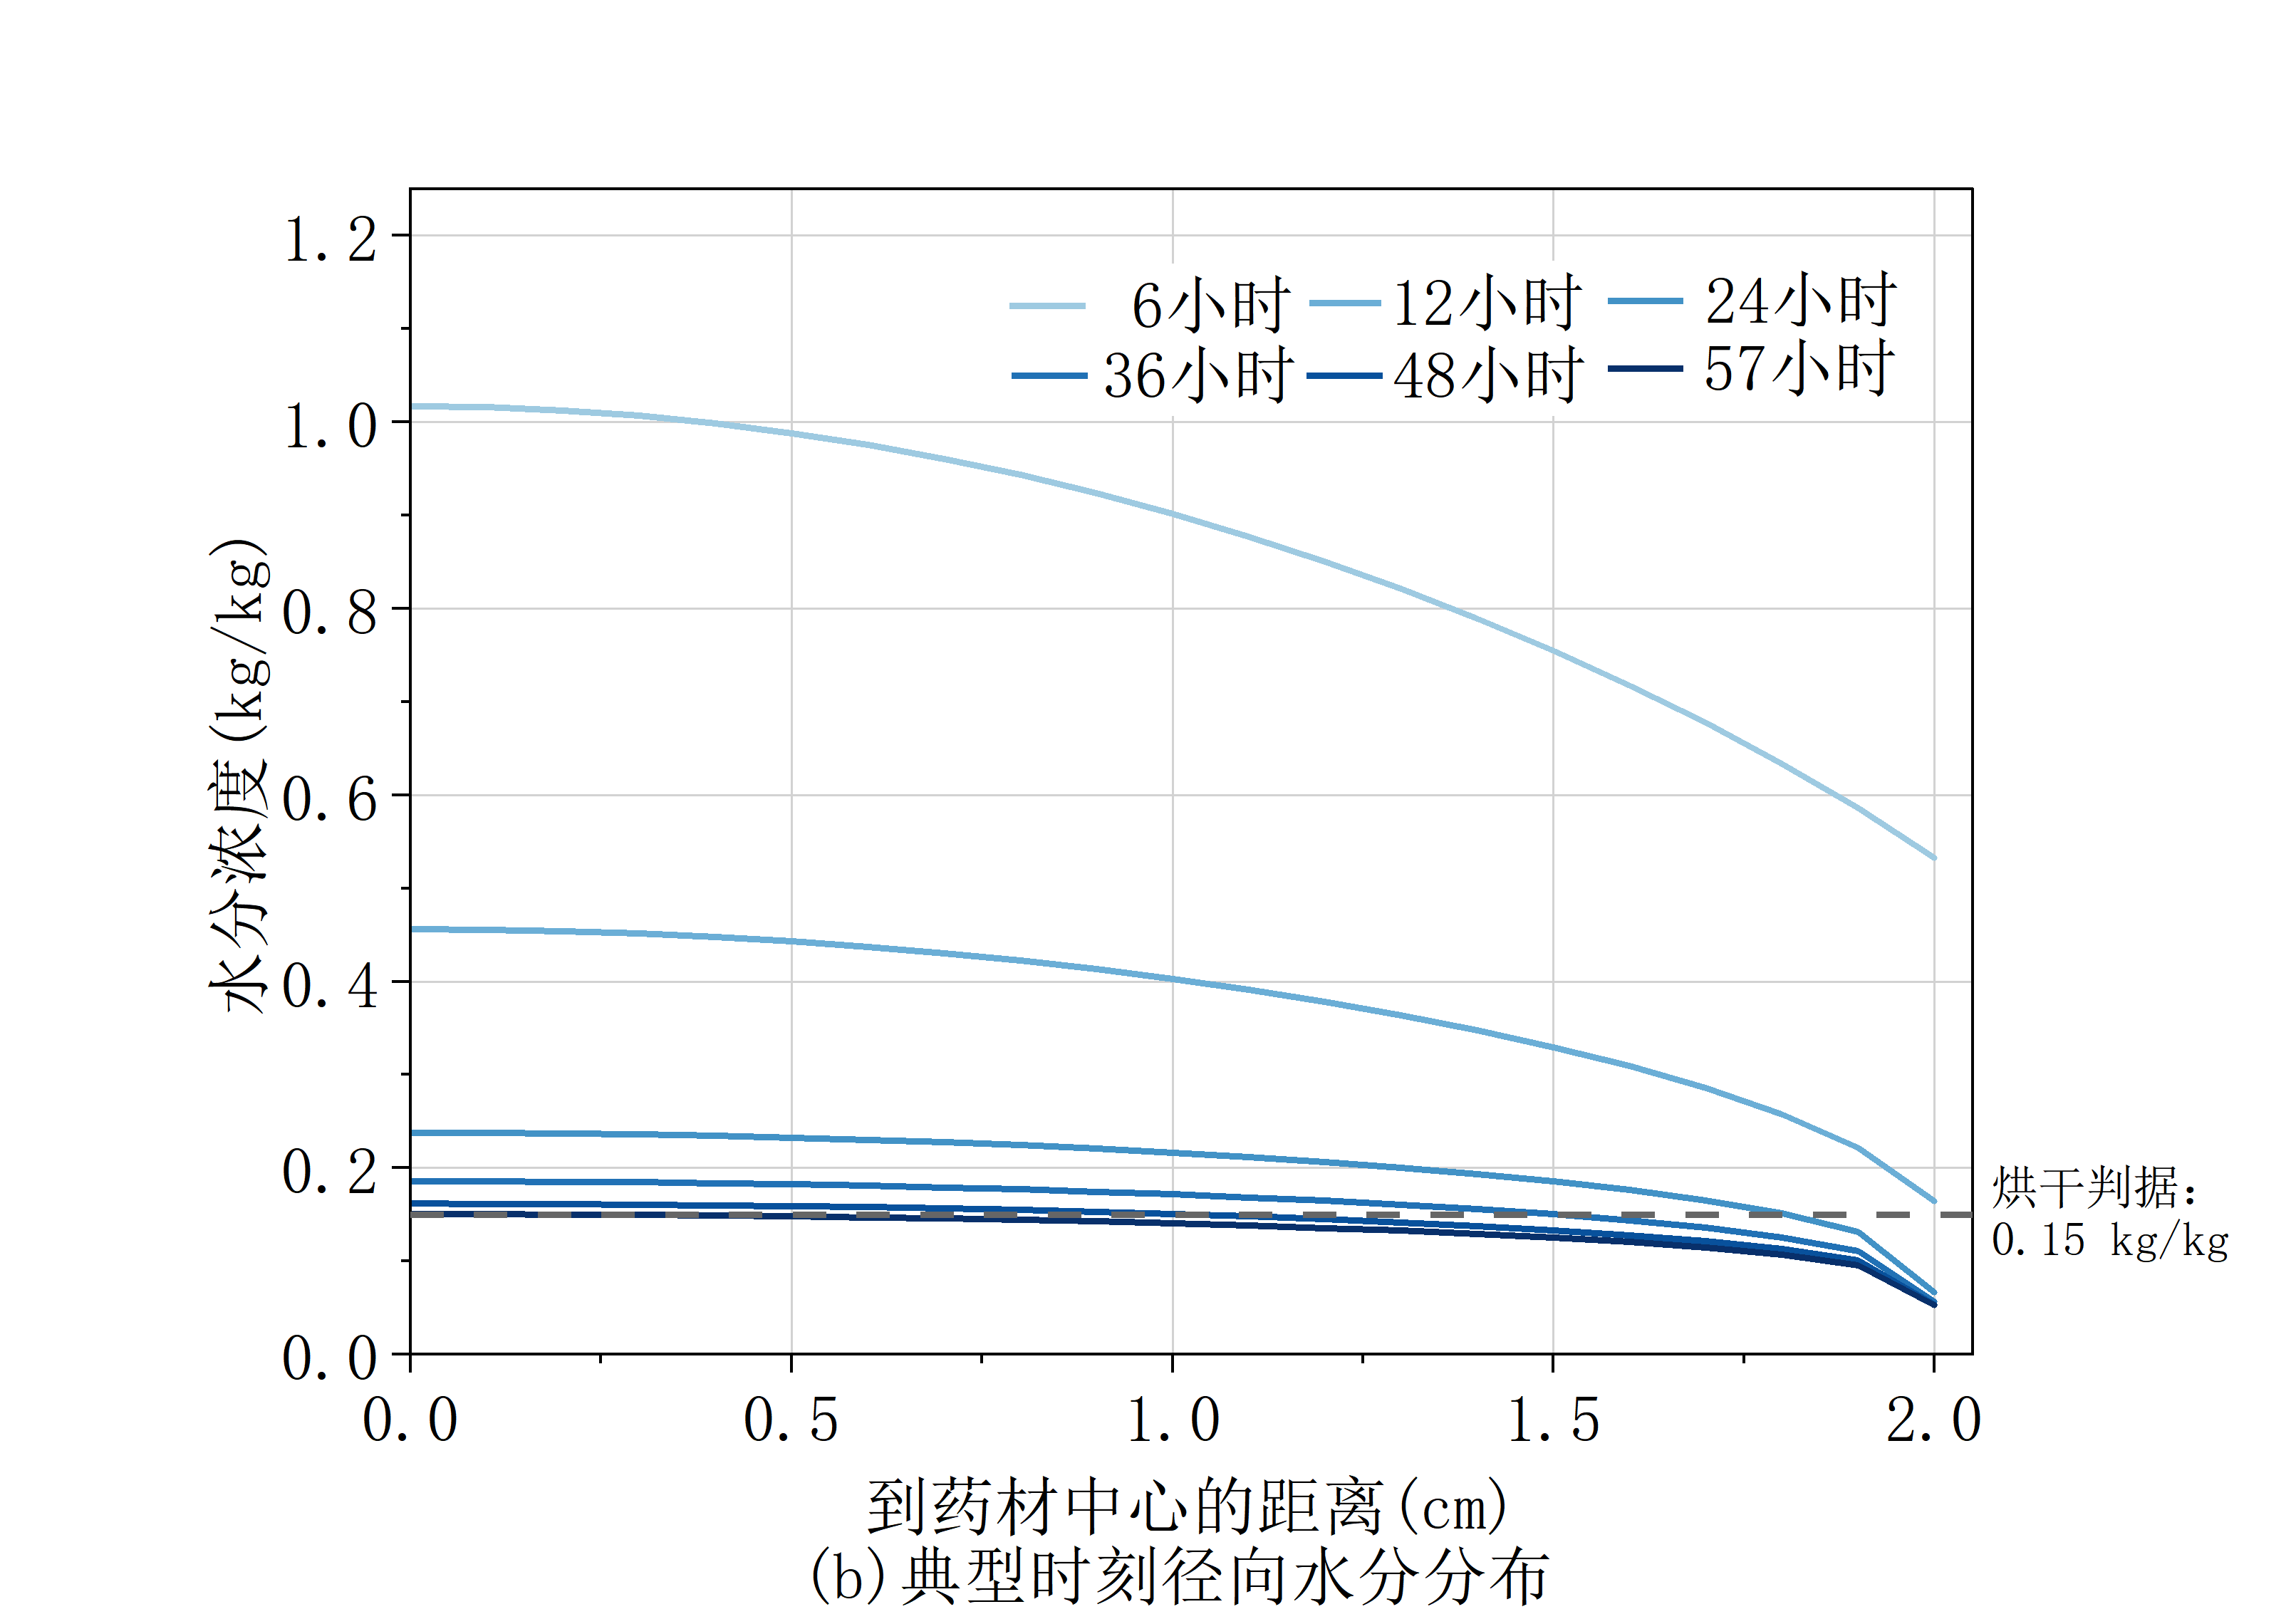
\includegraphics[trim={66.000bp 26.400bp 17.040bp 22.800bp},clip,
      width=0.49\unitlength]{图8(b).png}}}
\end{picture}
\caption{问题三全程干燥曲线与代表时刻的径向含水率分布}
\label{fig:p3-drying}
\end{figure}

\subsubsection{中心控制终点与径向差异}

在约$12.57\ \mathrm{h}$的保存结果中，表面含水率已低于$0.15\cunit$，
中心仍约为$0.4323\cunit$；图\ref{fig:p3-drying}(a)中的截面平均曲线也先于中心越过限值。
全域达标的临界时长则为$57.4721\ \mathrm{h}$，较表面达标滞后约$45 \mathrm{h}$。因此，\textbf{表面干燥不能代表整体达标，内部残余水分的缓慢迁出决定了烘干过程的长尾。}
结合第\ref{sec:p3-solution}节的逐节点核验，\textbf{中心是本算例的终点控制位置}。
$57.4721\ \mathrm{h}$的临界状态下，中心和表面含水率分别为
$0.1500\cunit$、$0.0527\cunit$，仍存在径向差异，
表明到达临界时刻并不意味着内部含水率已经均匀。


\section{问题四模型的建立与求解}
\label{sec:p4}
% 8.1：依据给定半径建立随骨架运动的热质模型，并映射至固定区间。
\subsection{模型建立}
\label{sec:p4-model}

本问引入失水收缩，从原始初态$t=0$起统一采用附录4物性，
描述骨架运动及水分相对骨架的扩散，并将运动区域映射至固定区间。

\subsubsection{半径函数与物性更新}

附件2给出了$0$至$72\ \mathrm{h}$内每隔$1800\ \mathrm{s}$的半径记录，
半径从$2.000\ \mathrm{cm}$逐渐减至$1.198\ \mathrm{cm}$。
沿用径向近似及长度不变假设，当前区域为$0\le r\le R(t)$。
将半径换算为米，以半径记录替换环境记录，沿用式\eqref{eq:p1-environment}的分段线性规则；
超出记录区间时按末值$R=0.01198\ \mathrm{m}$恒定延拓。

附录4的物性关系为
\begin{equation}
\begin{aligned}
  \rho(C)&=760+90C
    &&\mathrm{kg/m^3},\\
  c_p(C)&=1850+2150\frac{C}{C+1}
    &&\mathrm{J/(kg\,K)},\\
  k(C)&=0.12+0.20\frac{C}{C+1}
    &&\mathrm{W/(m\,K)},\\
  D(C,T_K)&=4.2\times10^{-4}
    \exp\!\left(-\frac{0.30}{C}\right)
    \exp\!\left(-\frac{3850}{T_K}\right)
    &&\mathrm{m^2/s},
\end{aligned}
\label{eq:p4-properties}
\end{equation}
其中$T_K=T+273.15$；热湿反馈结构沿用第\ref{sec:p2-model}节，
$R(t)$作为给定的几何输入。

\subsubsection{随骨架运动的热质守恒方程}

按假设\ref{assumption:shrinkage}，同一骨架物质点的$r/R(t)$保持不变。
在各半径插值区间内，骨架径向速度为
\begin{equation}
  v(r,t)=\frac{r}{R(t)}\frac{\dd R(t)}{\dd t}.
  \label{eq:p4-velocity}
\end{equation}
令$\rho_d$为单位当前体积内的干物质质量，水分质量密度为$\rho_d C$；
$\rho_d$与式\eqref{eq:p4-properties}中用于有效热容量的$\rho(C)$含义不同。
忽略干物质损失，以
$j=-\rho_d D(C,T_K)\frac{\partial C}{\partial r}$
表示相对骨架的径向水分通量，则骨架与水分连续性方程为
\begin{equation}
\begin{aligned}
  \frac{\partial\rho_d}{\partial t}
    +\frac{1}{r}\frac{\partial}{\partial r}(r\rho_d v)&=0,\\
  \frac{\partial(\rho_d C)}{\partial t}
    +\frac{1}{r}\frac{\partial}{\partial r}(r\rho_d C v)
    &=-\frac{1}{r}\frac{\partial(rj)}{\partial r}.
\end{aligned}
\label{eq:p4-continuity}
\end{equation}
第二式减去第一式的$C$倍，消去骨架压缩引起的共同密度变化。
采用同一时刻$\rho_d$径向均匀的有效传输闭合，约去$\rho_d$，
结合显热传导近似得到运动区域上的控制方程：
\begin{equation}
\left\{
\begin{aligned}
  \rho(C)c_p(C)\left(\frac{\partial T}{\partial t}
    +v\frac{\partial T}{\partial r}\right)
    &=\frac{1}{r}\frac{\partial}{\partial r}
      \left[rk(C)\frac{\partial T}{\partial r}\right],\\
  \frac{\partial C}{\partial t}+v\frac{\partial C}{\partial r}
    &=\frac{1}{r}\frac{\partial}{\partial r}
      \left[rD(C,T_K)\frac{\partial C}{\partial r}\right],
\end{aligned}
\right.
\quad 0<r<R(t).
\label{eq:p4-moving-pde}
\end{equation}
左端为随骨架的变化率。
干基含水率是水与干物质的质量比，单纯收缩不会使其自动增大，
故不另加体积浓度形式的压缩源项。

\subsubsection{物质坐标下的固定区域模型}

引入物质坐标及对应场量
\[
  \xi=\frac{r}{R(t)},\qquad
  \widetilde T(\xi,t)=T(R(t)\xi,t),\qquad
  \widetilde C(\xi,t)=C(R(t)\xi,t).
\]
其中$\xi=0,1$分别对应中心和实际表面，固定$\xi$即跟随同一骨架物质点。
如图\ref{fig:p4-schematic}所示，收缩过程中同一物质点的物理位置随$R(t)$改变，
而其归一化坐标保持不变，从而将变化的物理区域映射为固定计算区间$[0,1]$。

\pfig{图9.png}{0.90}{问题四收缩物理区域与固定物质坐标区域的映射示意图}{fig:p4-schematic}

对$u=T$或$C$应用链式法则，得
\begin{equation}
  \frac{\partial\widetilde u}{\partial t}
    =\frac{\partial u}{\partial t}
      +v\frac{\partial u}{\partial r},\qquad
  \frac{\partial u}{\partial r}
    =\frac{1}{R(t)}\frac{\partial\widetilde u}{\partial\xi}.
  \label{eq:p4-coordinate-transform}
\end{equation}
代入式\eqref{eq:p4-moving-pde}并乘以$R^2(t)$，得固定区间上的方程：
\begin{equation}
\left\{
\begin{aligned}
  R^2(t)\rho(\widetilde C)c_p(\widetilde C)
    \frac{\partial\widetilde T}{\partial t}
    &=\frac{1}{\xi}\frac{\partial}{\partial\xi}
      \left[\xi k(\widetilde C)
      \frac{\partial\widetilde T}{\partial\xi}\right],\\
  R^2(t)\frac{\partial\widetilde C}{\partial t}
    &=\frac{1}{\xi}\frac{\partial}{\partial\xi}
      \left[\xi D(\widetilde C,\widetilde T_K)
      \frac{\partial\widetilde C}{\partial\xi}\right],
\end{aligned}
\right.
\quad 0<\xi<1,
\label{eq:p4-fixed-pde}
\end{equation}
其中$\widetilde T_K=\widetilde T+273.15$。
骨架运动已包含在固定$\xi$处的时间导数内，尺寸变化通过$R^2(t)$进入储存项。

\subsubsection{初边条件与全域达标判据}

初始温湿状态沿用式\eqref{eq:p1-initial}，且$R(0)=R_0$；
环境函数沿用式\eqref{eq:p1-environment}的插值及前文的恒定延拓，$h$、$h_m$不变。

记$T_s=\widetilde T(1,t)$、$C_s=\widetilde C(1,t)$及$T_{K,s}=T_s+273.15$。
由中心对称及相对骨架的表面传递条件，经式\eqref{eq:p4-coordinate-transform}变换得
\begin{equation}
\left\{
\begin{aligned}
  \left.\frac{\partial\widetilde T}{\partial\xi}\right|_{\xi=0}
    &=\left.\frac{\partial\widetilde C}{\partial\xi}\right|_{\xi=0}=0,\\
  -k(C_s)\left.\frac{\partial\widetilde T}{\partial\xi}\right|_{\xi=1}
    &=R(t)h[T_s-T_a(t)],\\
  -D(C_s,T_{K,s})\left.\frac{\partial\widetilde C}{\partial\xi}\right|_{\xi=1}
    &=R(t)h_m[C_s-C_a(t)].
\end{aligned}
\right.
\label{eq:p4-boundary}
\end{equation}
表面交换项含$R(t)$，与储存项中的$R^2(t)$不同；
固定域方程及边界条件均无需对半径记录额外求导。

全域最大含水率为
\begin{equation}
  C_{\max}(t)=\max_{0\le r\le R(t)}C(r,t)
    =\max_{0\le\xi\le1}\widetilde C(\xi,t),
  \label{eq:p4-maximum}
\end{equation}
临界烘干时间$t_*$沿用式\eqref{eq:p3-endpoint}的判据。

% 8.2：与code/p4.py主模型B的固定xi网格、中点半径及同步Picard一致。
% 表6沿用既有生产结果，已核对NPZ、Excel与原结果表；本次写作未重算PDE。
\subsection{模型求解}
\label{sec:p4-solution}

对式\eqref{eq:p4-fixed-pde}沿用有限体积离散与双场Picard迭代，
将半径变化纳入系数，并将结果映射至题定物理位置。

\subsubsection{固定坐标离散与时变系数的组装}

在$0=\xi_0<\xi_1<\cdots<\xi_N=1$上设置固定网格，
记$T_i^n\approx\widetilde T(\xi_i,t^n)$、
$C_i^n\approx\widetilde C(\xi_i,t^n)$。
控制面取相邻节点中点，两端为$\xi_{-1/2}=0$、$\xi_{N+1/2}=1$。
无量纲积分权重与本步半径为
\begin{equation}
  \widehat V_i=\frac{\xi_{i+1/2}^2-\xi_{i-1/2}^2}{2},
  \qquad
  R_m^n=\frac{R(t^n)+R(t^{n+1})}{2}.
  \label{eq:p4-discrete-geometry}
\end{equation}
其中$\widehat V_i$由固定网格确定，$R_m^n$在本步各轮迭代中保持不变。

各轮物性均按式\eqref{eq:p2-midpoint}的时间中点状态代入式\eqref{eq:p4-properties}计算。
面导通系数沿用式\eqref{eq:p1-fvm-coefficients}中的$G$定义，
将$r$替换为$\xi$，$\Gamma$分别取$k$、$D$，面物性仍取算术平均。
新增的时间项与表面交换系数为
\begin{equation}
\begin{aligned}
  m_{T,i}^{(\ell)}
    &=\frac{(R_m^n)^2(\rho c_p)_i^{(\ell)}\widehat V_i}{\Delta t_n},
  &m_{C,i}
    &=\frac{(R_m^n)^2\widehat V_i}{\Delta t_n},\\
  B_T&=R_m^n h,
  &B_C&=R_m^n h_m.
\end{aligned}
\label{eq:p4-discrete-coefficients}
\end{equation}
其中$(\rho c_p)_i^{(\ell)}$表示该中点状态下的$\rho(C)c_p(C)$。
水分时间项为$m_{C,i}(C_i^{n+1}-C_i^n)$，即$(R_m^n)^2$乘场量增量，
不能改写为$R^2C$的时间差分。

将上述系数代入式\eqref{eq:p1-linear-system}组装两场三对角系统；
同轮新、旧层通量共用中点物性及半径系数，环境值按式\eqref{eq:p1-surface-row}加权进入右端。

\subsubsection{同步迭代与临界时刻定位}

线性求解器、双场同步迭代及收敛条件沿用第\ref{sec:p2-solution}节，
分段步长与仅最初两步隐式启动的设置沿用第\ref{sec:p3-solution}节。
在$\xi$方向设置882个节点，并在$0.975<\xi\le1$内加密；
实际位置为$r_i(t)=R(t)\xi_i$，环境与半径插值折点均落在时间层上。
表面附近失水较快、含水率梯度较大，局部加密可更准确地分辨这一薄层内的场量变化及表面通量。

每步收敛后按式\eqref{eq:p4-maximum}检查全部节点；
中心与网格最大含水率之差始终不超过$10^{-12}\cunit$，故本算例由中心控制终点。
首次穿越阈值时，按式\eqref{eq:p3-event-interpolation}对未舍入结果线性插值，
得到$t_*$及整条$\xi$方向含水率分布，并计算$R(t_*)$。

\subsubsection{烘干时长与结果输出}

计算得到
\begin{equation*}
  \boxed{t_*\approx51.0905\ \mathrm{h}},\qquad
  R(t_*)=1.200\ \mathrm{cm}.
\end{equation*}
对$r_q\le R(t)$，映射至$\xi_q=r_q/R(t)$并在相邻节点间线性插值；
域外位置无内部场值，实际表面取$\xi_N=1$处的结果。
每隔$6\ \mathrm{h}$及临界时刻的题定位置含水率见表\ref{tab:p4C}，
横线表示域外位置，末列为实际表面。

\begin{table}[!htbp]
  \centering
  \caption{考虑径向收缩时药材烘干过程的水分浓度（单位：$\mathrm{kg/kg}$）}
  \label{tab:p4C}
  \begin{tabularx}{\textwidth}{@{}C{0.22\textwidth}YYYYY@{}}
    \toprule
    \multirow{2}{*}{时间/$\mathrm{h}$}&\multicolumn{4}{c}{到药材中心的距离/$\mathrm{cm}$}
      &\multirow{2}{*}{药材表面}\\
    \cmidrule(lr){2-5}
    &0&0.5&1&1.5&\\
    \midrule
    6  &1.7196&1.5377&1.0226&---&0.4207\\
    12 &0.7377&0.6546&0.4083&---&0.1670\\
    18 &0.4087&0.3686&0.2397&---&0.0892\\
    24 &0.2851&0.2611&0.1790&---&0.0673\\
    30 &0.2263&0.2094&0.1493&---&0.0595\\
    36 &0.1928&0.1797&0.1317&---&0.0560\\
    42 &0.1712&0.1604&0.1200&---&0.0541\\
    48 &0.1561&0.1468&0.1116&---&0.0530\\
    \mbox{\textbf{51.0905（结束）}}
       &\textbf{0.1500}&\textbf{0.1413}&\textbf{0.1081}&\textbf{---}&\textbf{0.0526}\\
    \bottomrule
  \end{tabularx}
\end{table}

表末行为$C_{\max}=C_*$的临界状态；继续计算至其后的首个整分钟\textbf{$183960\ \mathrm{s}$}，
此时未舍入的$C_{\max}<C_*$。
按$60\ \mathrm{s}$间隔及$r=0,0.1,\ldots,2.0\ \mathrm{cm}$位置，
以四位小数写入\texttt{result4.xlsx}；域外留空，另设“药材表面”列。

% 8.3：依据表6与同源采样场分析收缩过程；图8(a)使用用户更新的PNG，(b)沿用原数据重绘，图9沿用原图。
\subsection{结果分析}
\label{sec:p4-analysis}

结合表\ref{tab:p4C}及图\ref{fig:p4-drying}分析收缩过程，
并通过图\ref{fig:p34-comparison}与固定尺寸工况比较，考察尺寸变化和物性更新的共同影响。

\subsubsection{收缩过程与终点状态}

图\ref{fig:p4-drying}(a)中的黑色曲线表示实际表面$r=R(t)$，
其下方为当时的药材区域。
$6\ \mathrm{h}$时半径已由$2.000\ \mathrm{cm}$降至$1.374\ \mathrm{cm}$，
$36\ \mathrm{h}$时接近$1.200\ \mathrm{cm}$，但中心含水率仍为$0.1928\cunit$。
这表明收缩主要发生在前期，尺寸趋稳早于全域达标，不能以半径趋稳判断干燥结束。

\begin{figure}[!htbp]
\centering
% 保持原图8的0.98\textwidth宽度及275.6785/636.93875高宽比。
% (a)分开裁剪主图、标题与色条；结束时间移至轴框内右上方空白处，避免与色条标题重叠。
% 各部分仅指定一个缩放尺寸，保持原始比例；trim按(a)源PNG的300 dpi换算。
% (b)沿用原始数据，以宋体及Times New Roman重绘，保留原大小与位置。
\setlength{\unitlength}{0.98\textwidth}
\begin{picture}(1,0.432817912)
  % (a)水分场、表面曲线及坐标轴。
  \put(-0.001114244,0.008490525){\makebox(0,0)[lb]{%
    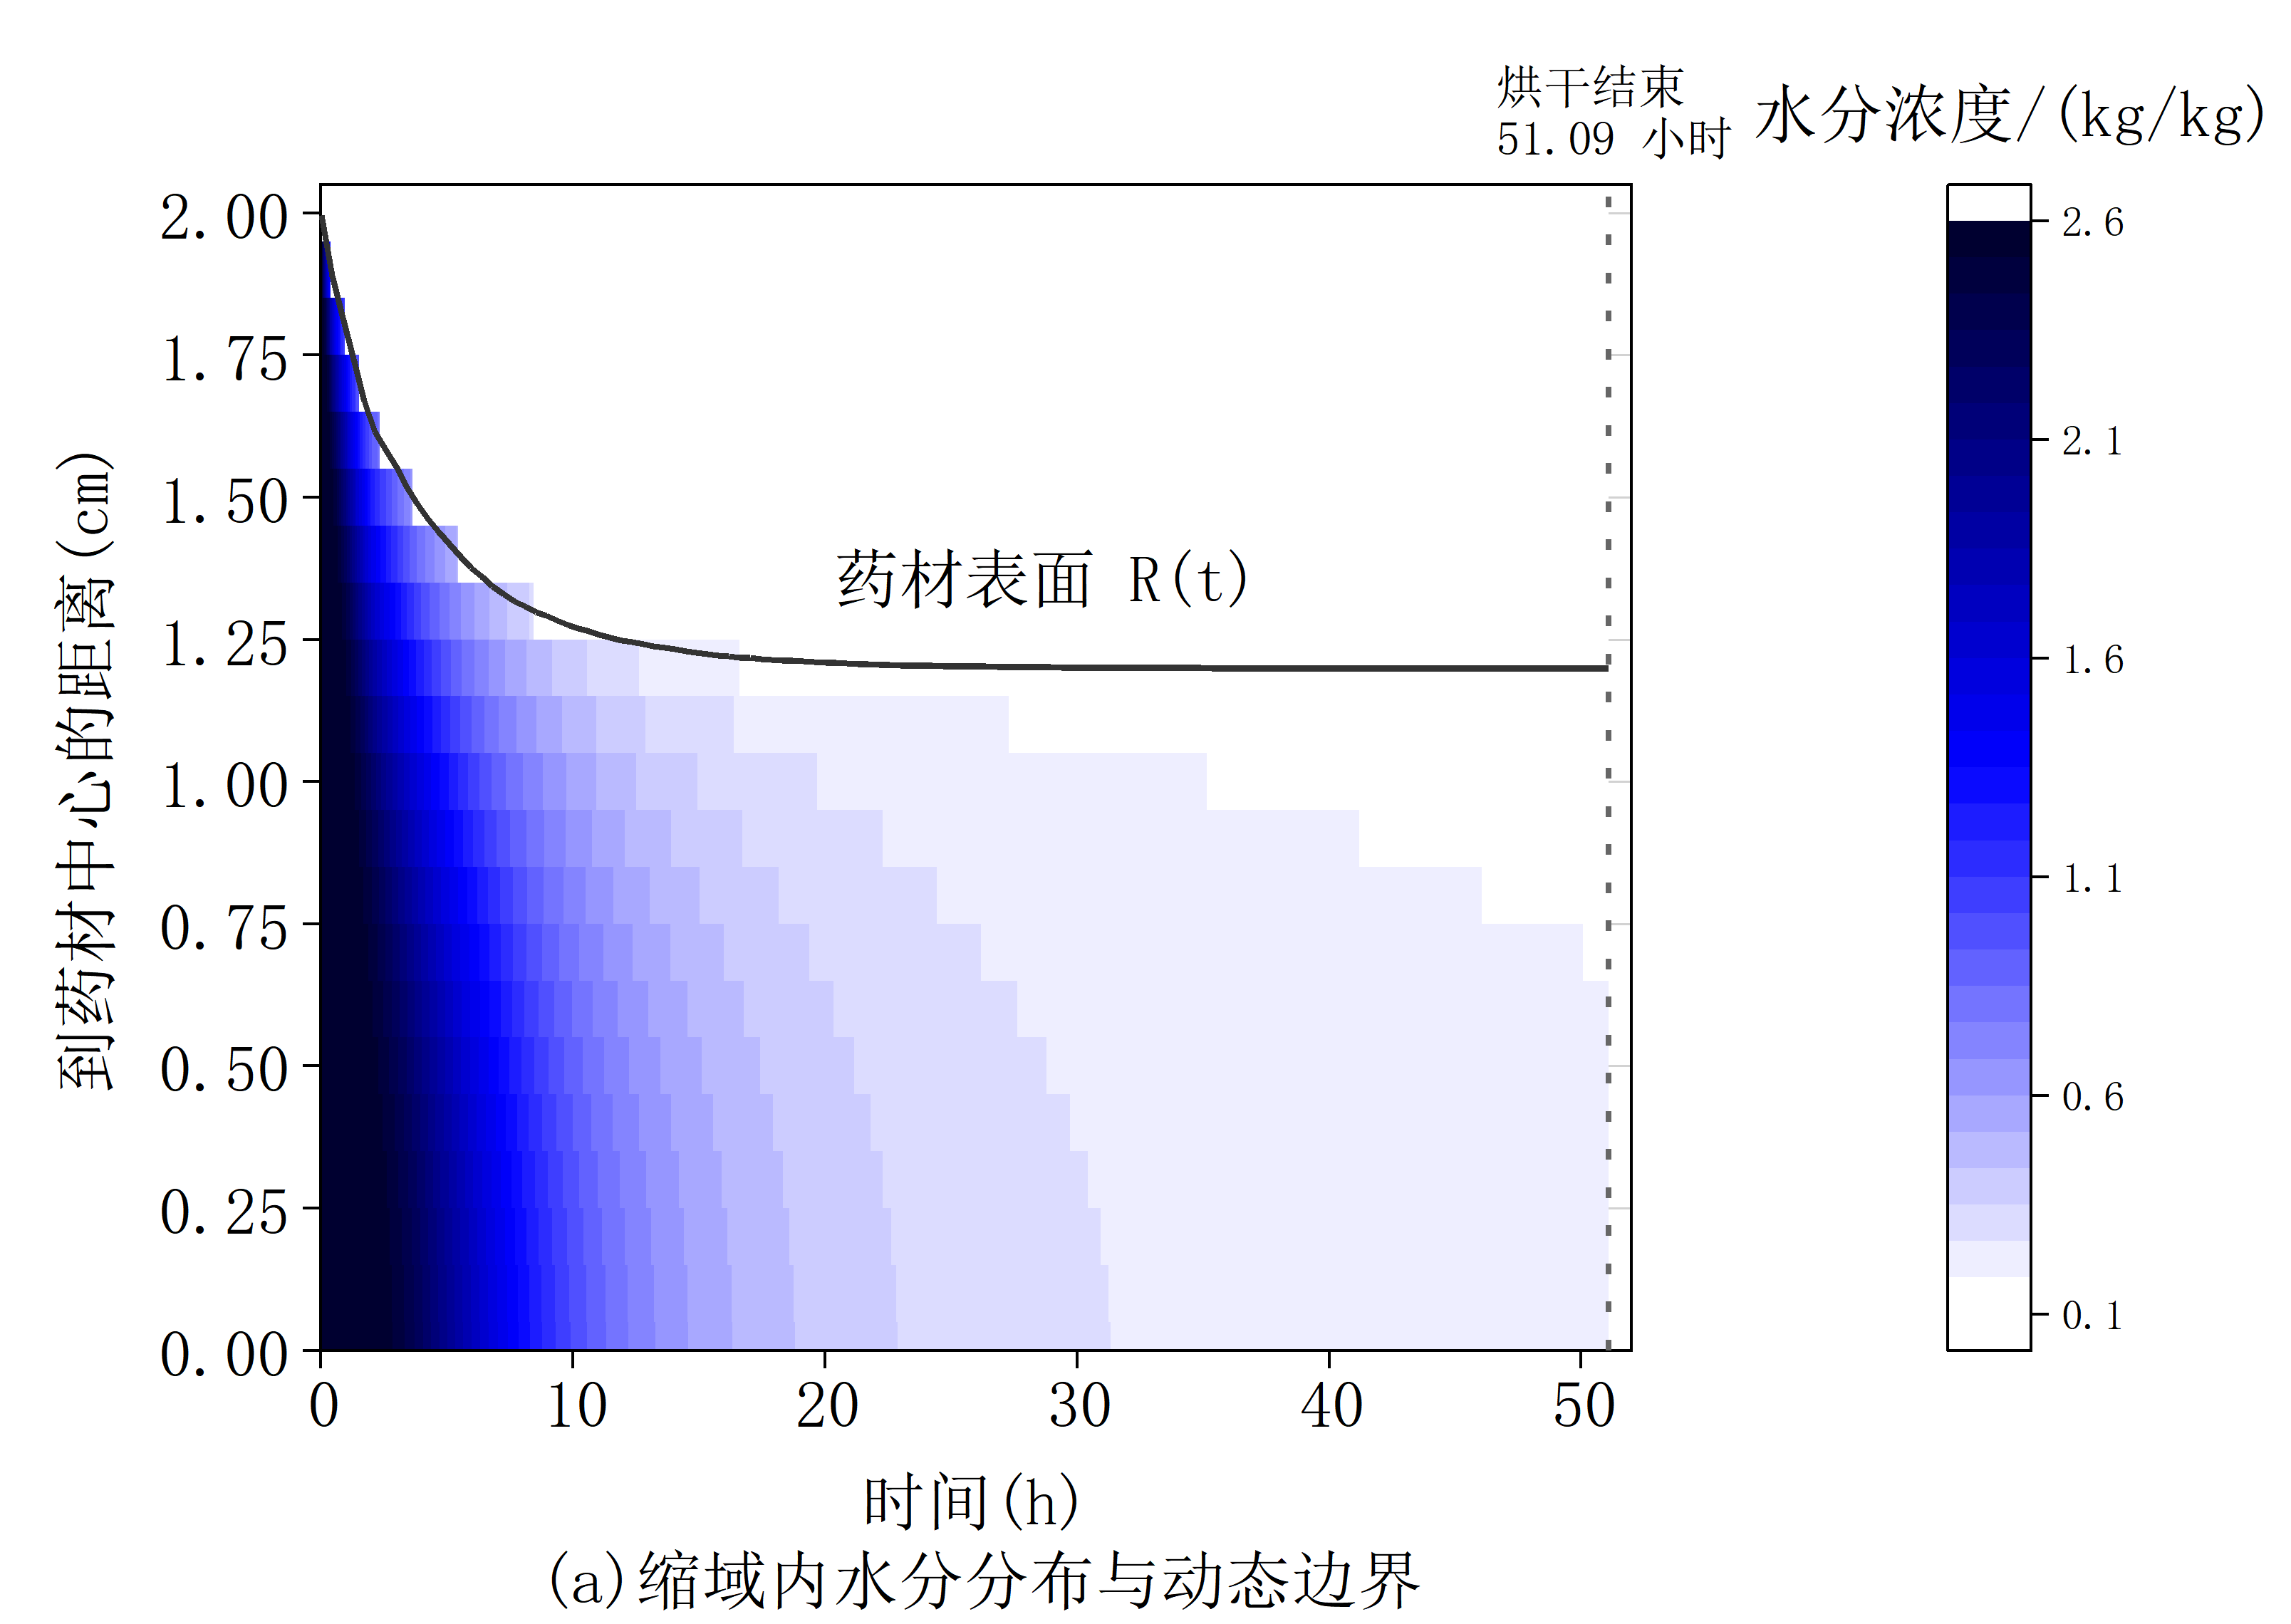
\includegraphics[trim={14.400bp 27.600bp 212.640bp 58.800bp},clip,
      height=0.387954163\unitlength]{图10(a).png}}}
  \put(0.074658053,0.395434391){\makebox(0,0)[lb]{%
    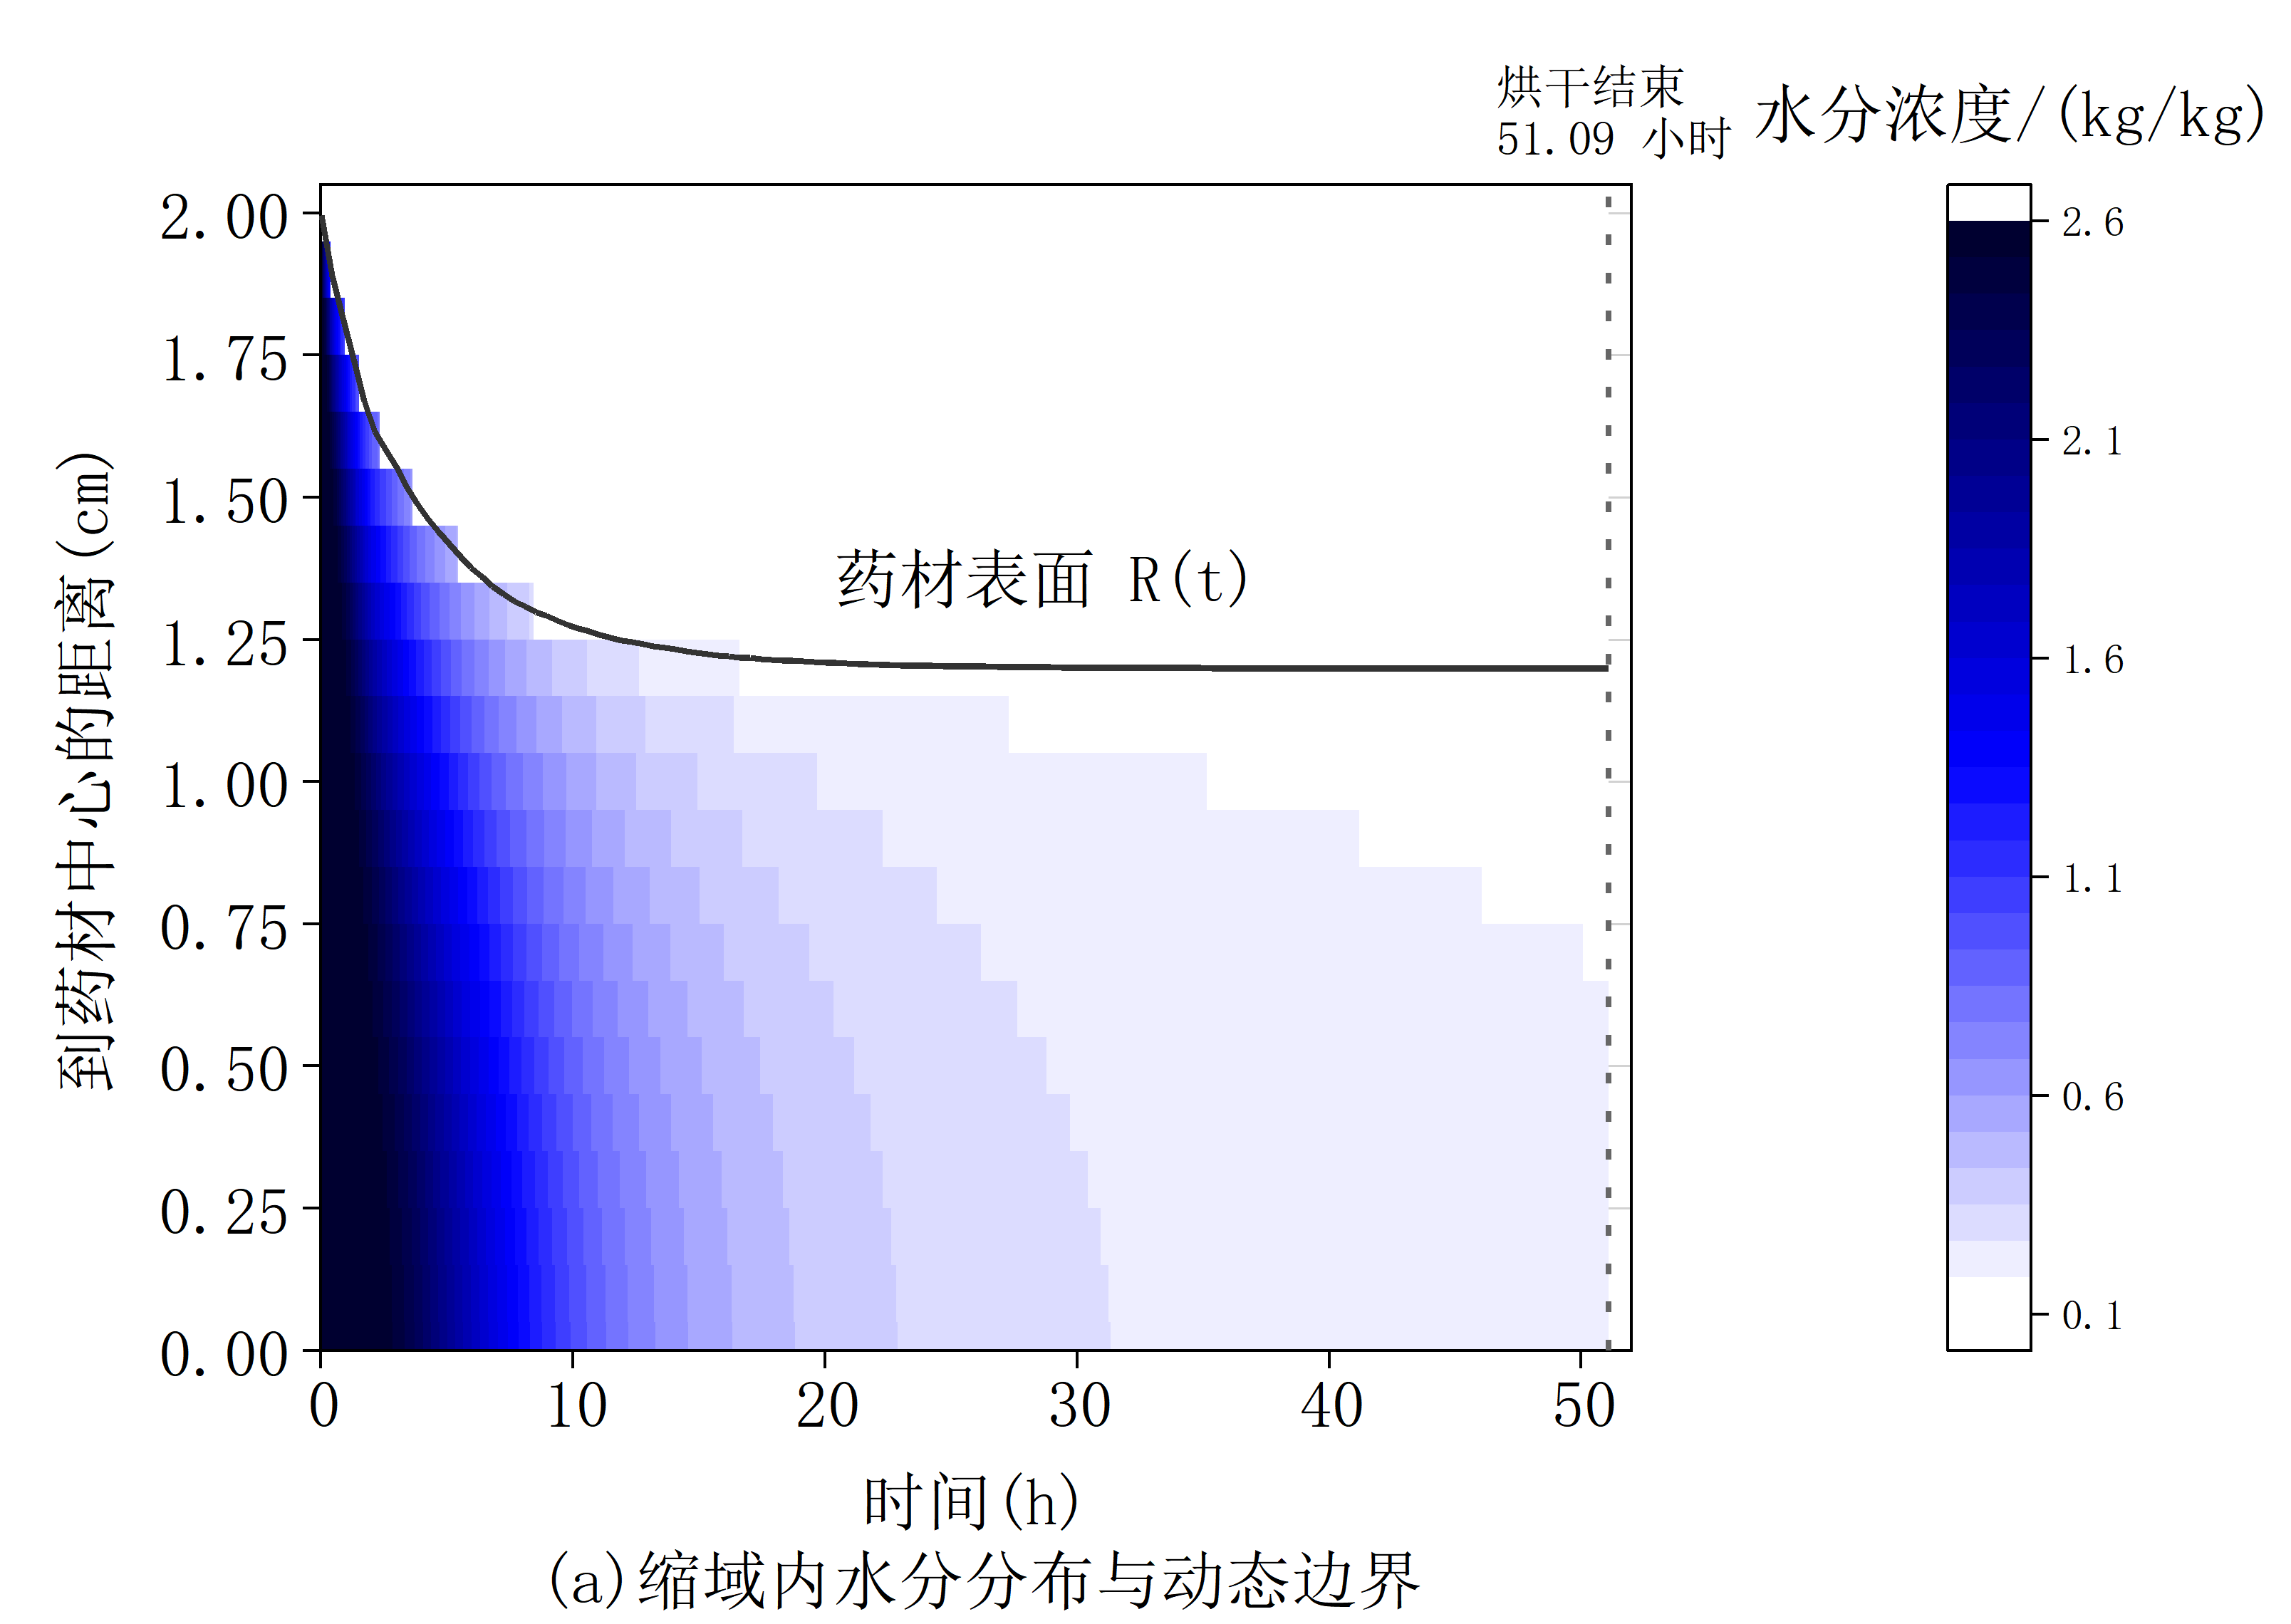
\includegraphics[trim={104.400bp 487.200bp 367.440bp 34.800bp},clip,
      height=0.021216243\unitlength]{图10(a).png}}}
  % (a)色条及单位。
  \put(0.461073868,0.060015687){\makebox(0,0)[lb]{%
    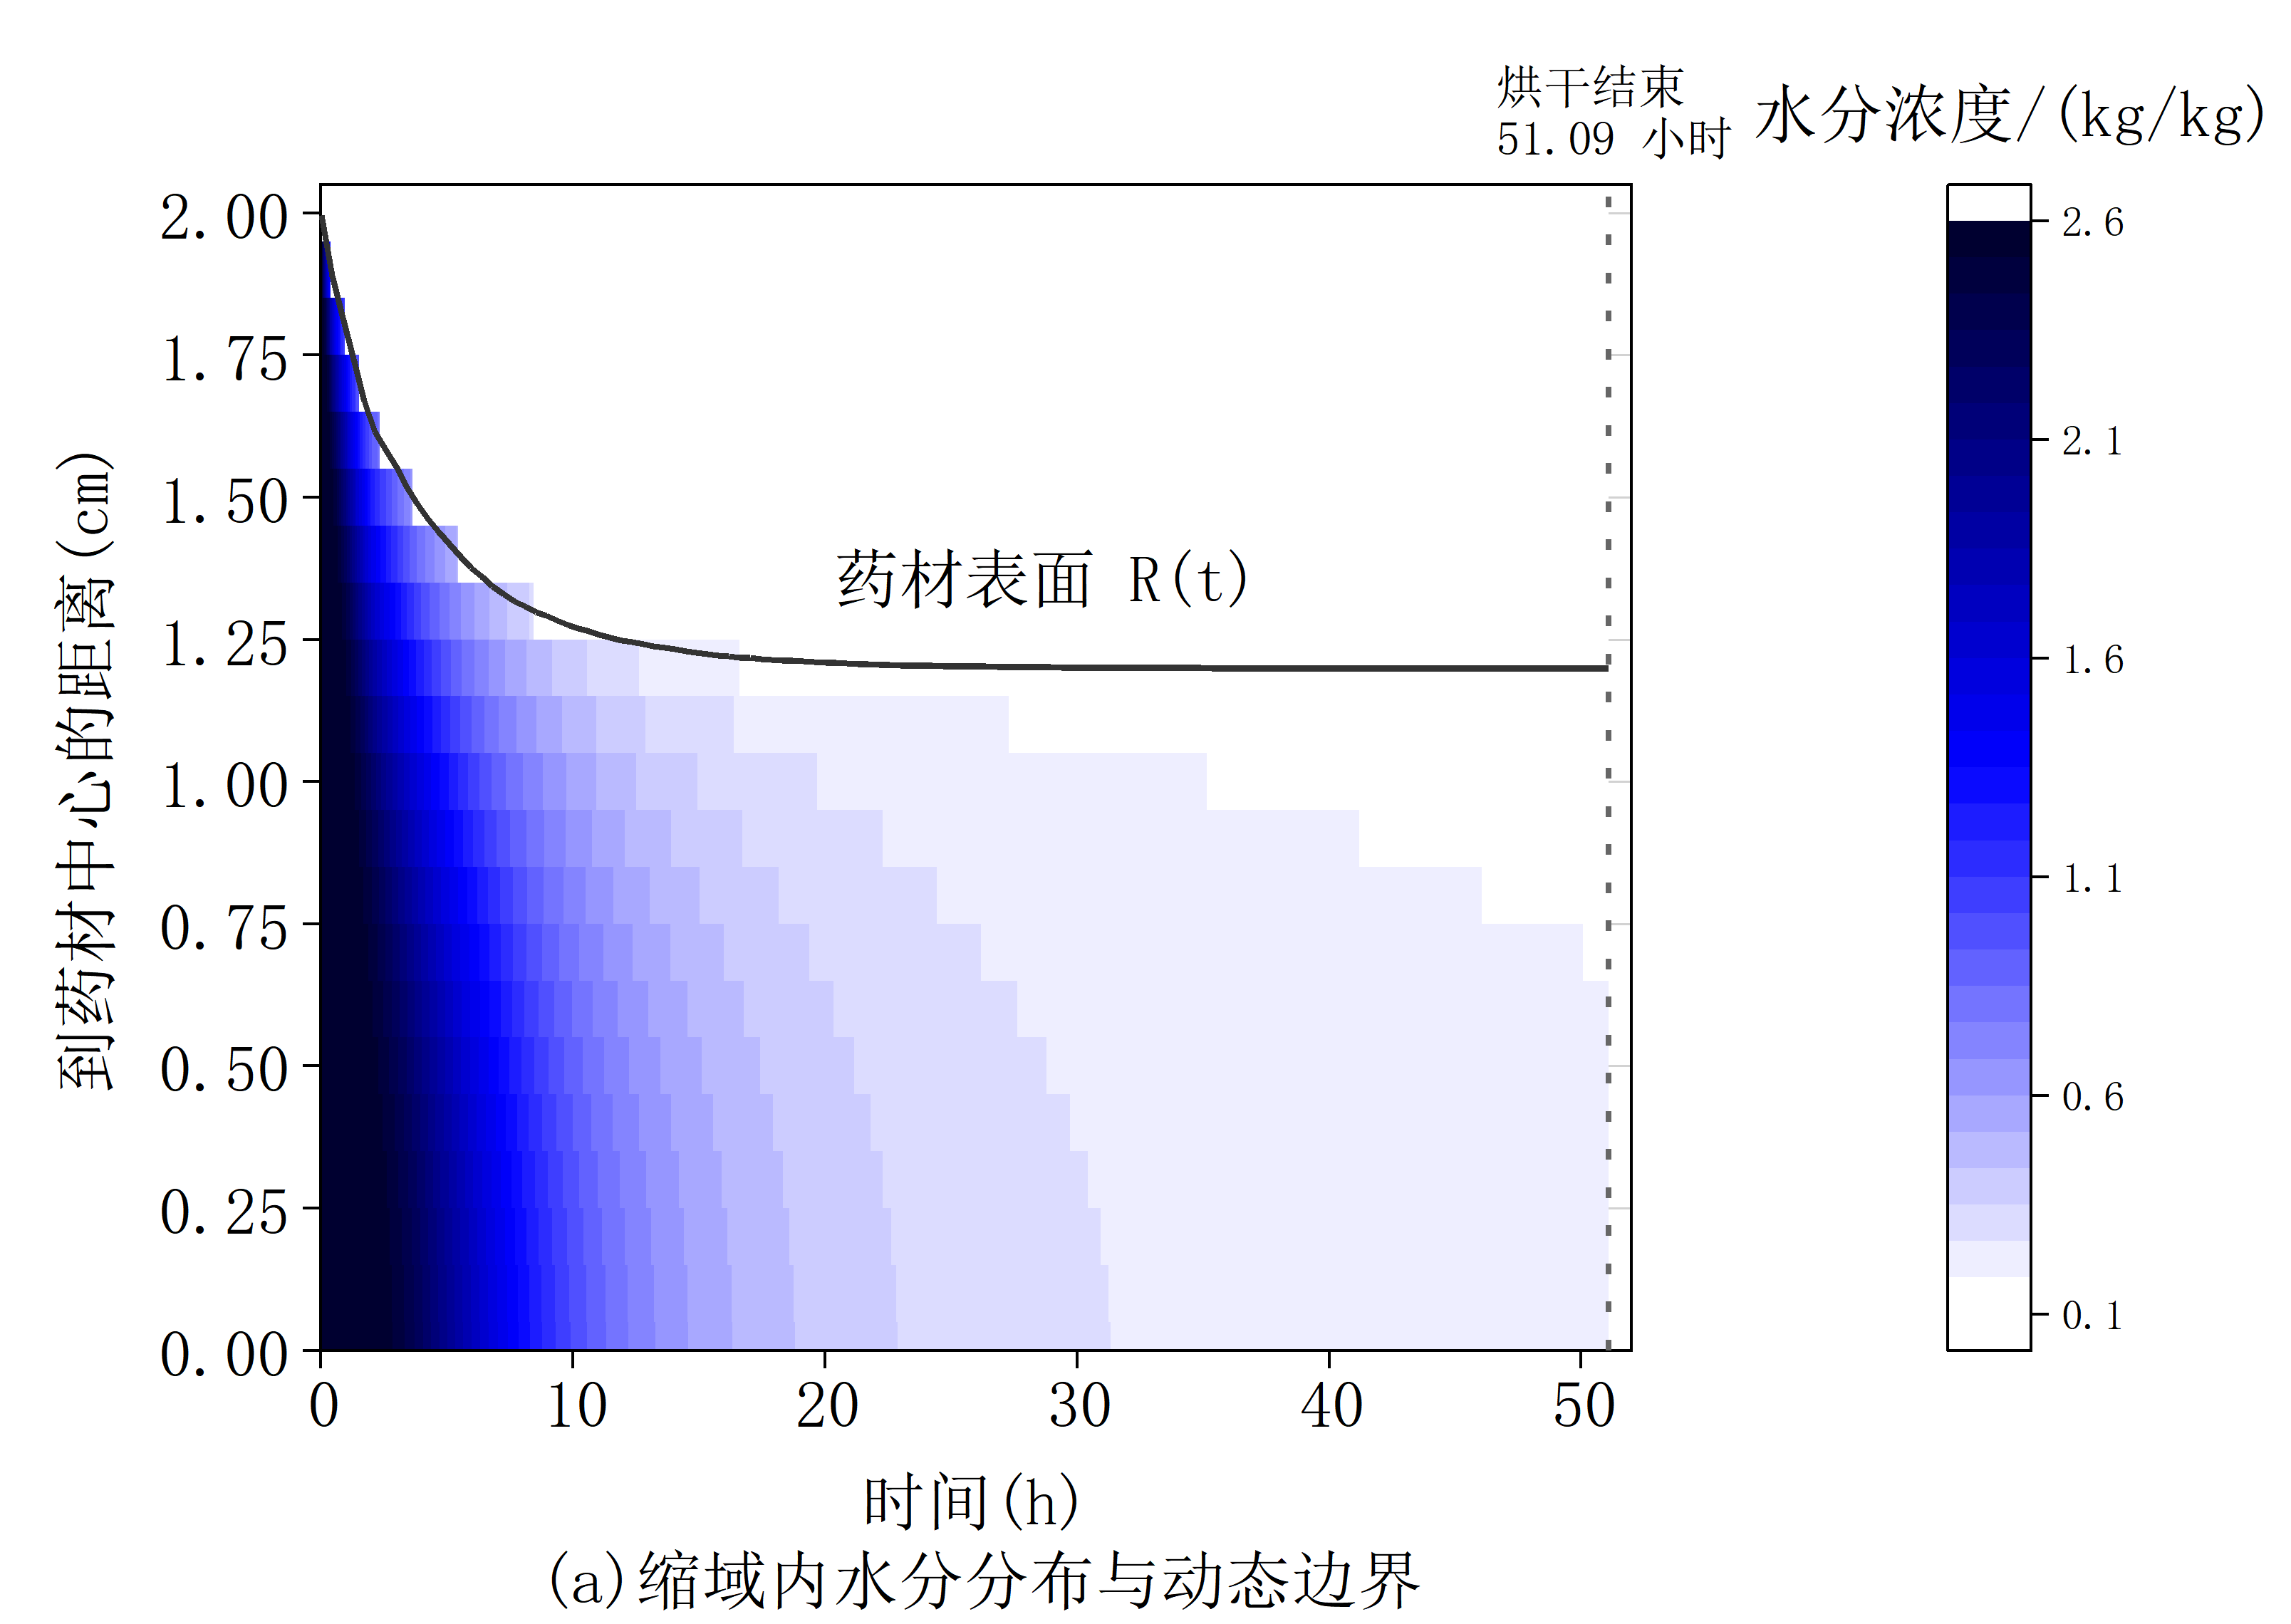
\includegraphics[trim={651.600bp 88.800bp 24.240bp 58.800bp},clip,
      height=0.336429001\unitlength]{图10(a).png}}}
  \put(0.396278884,0.402506472){\makebox(0,0)[lb]{%
    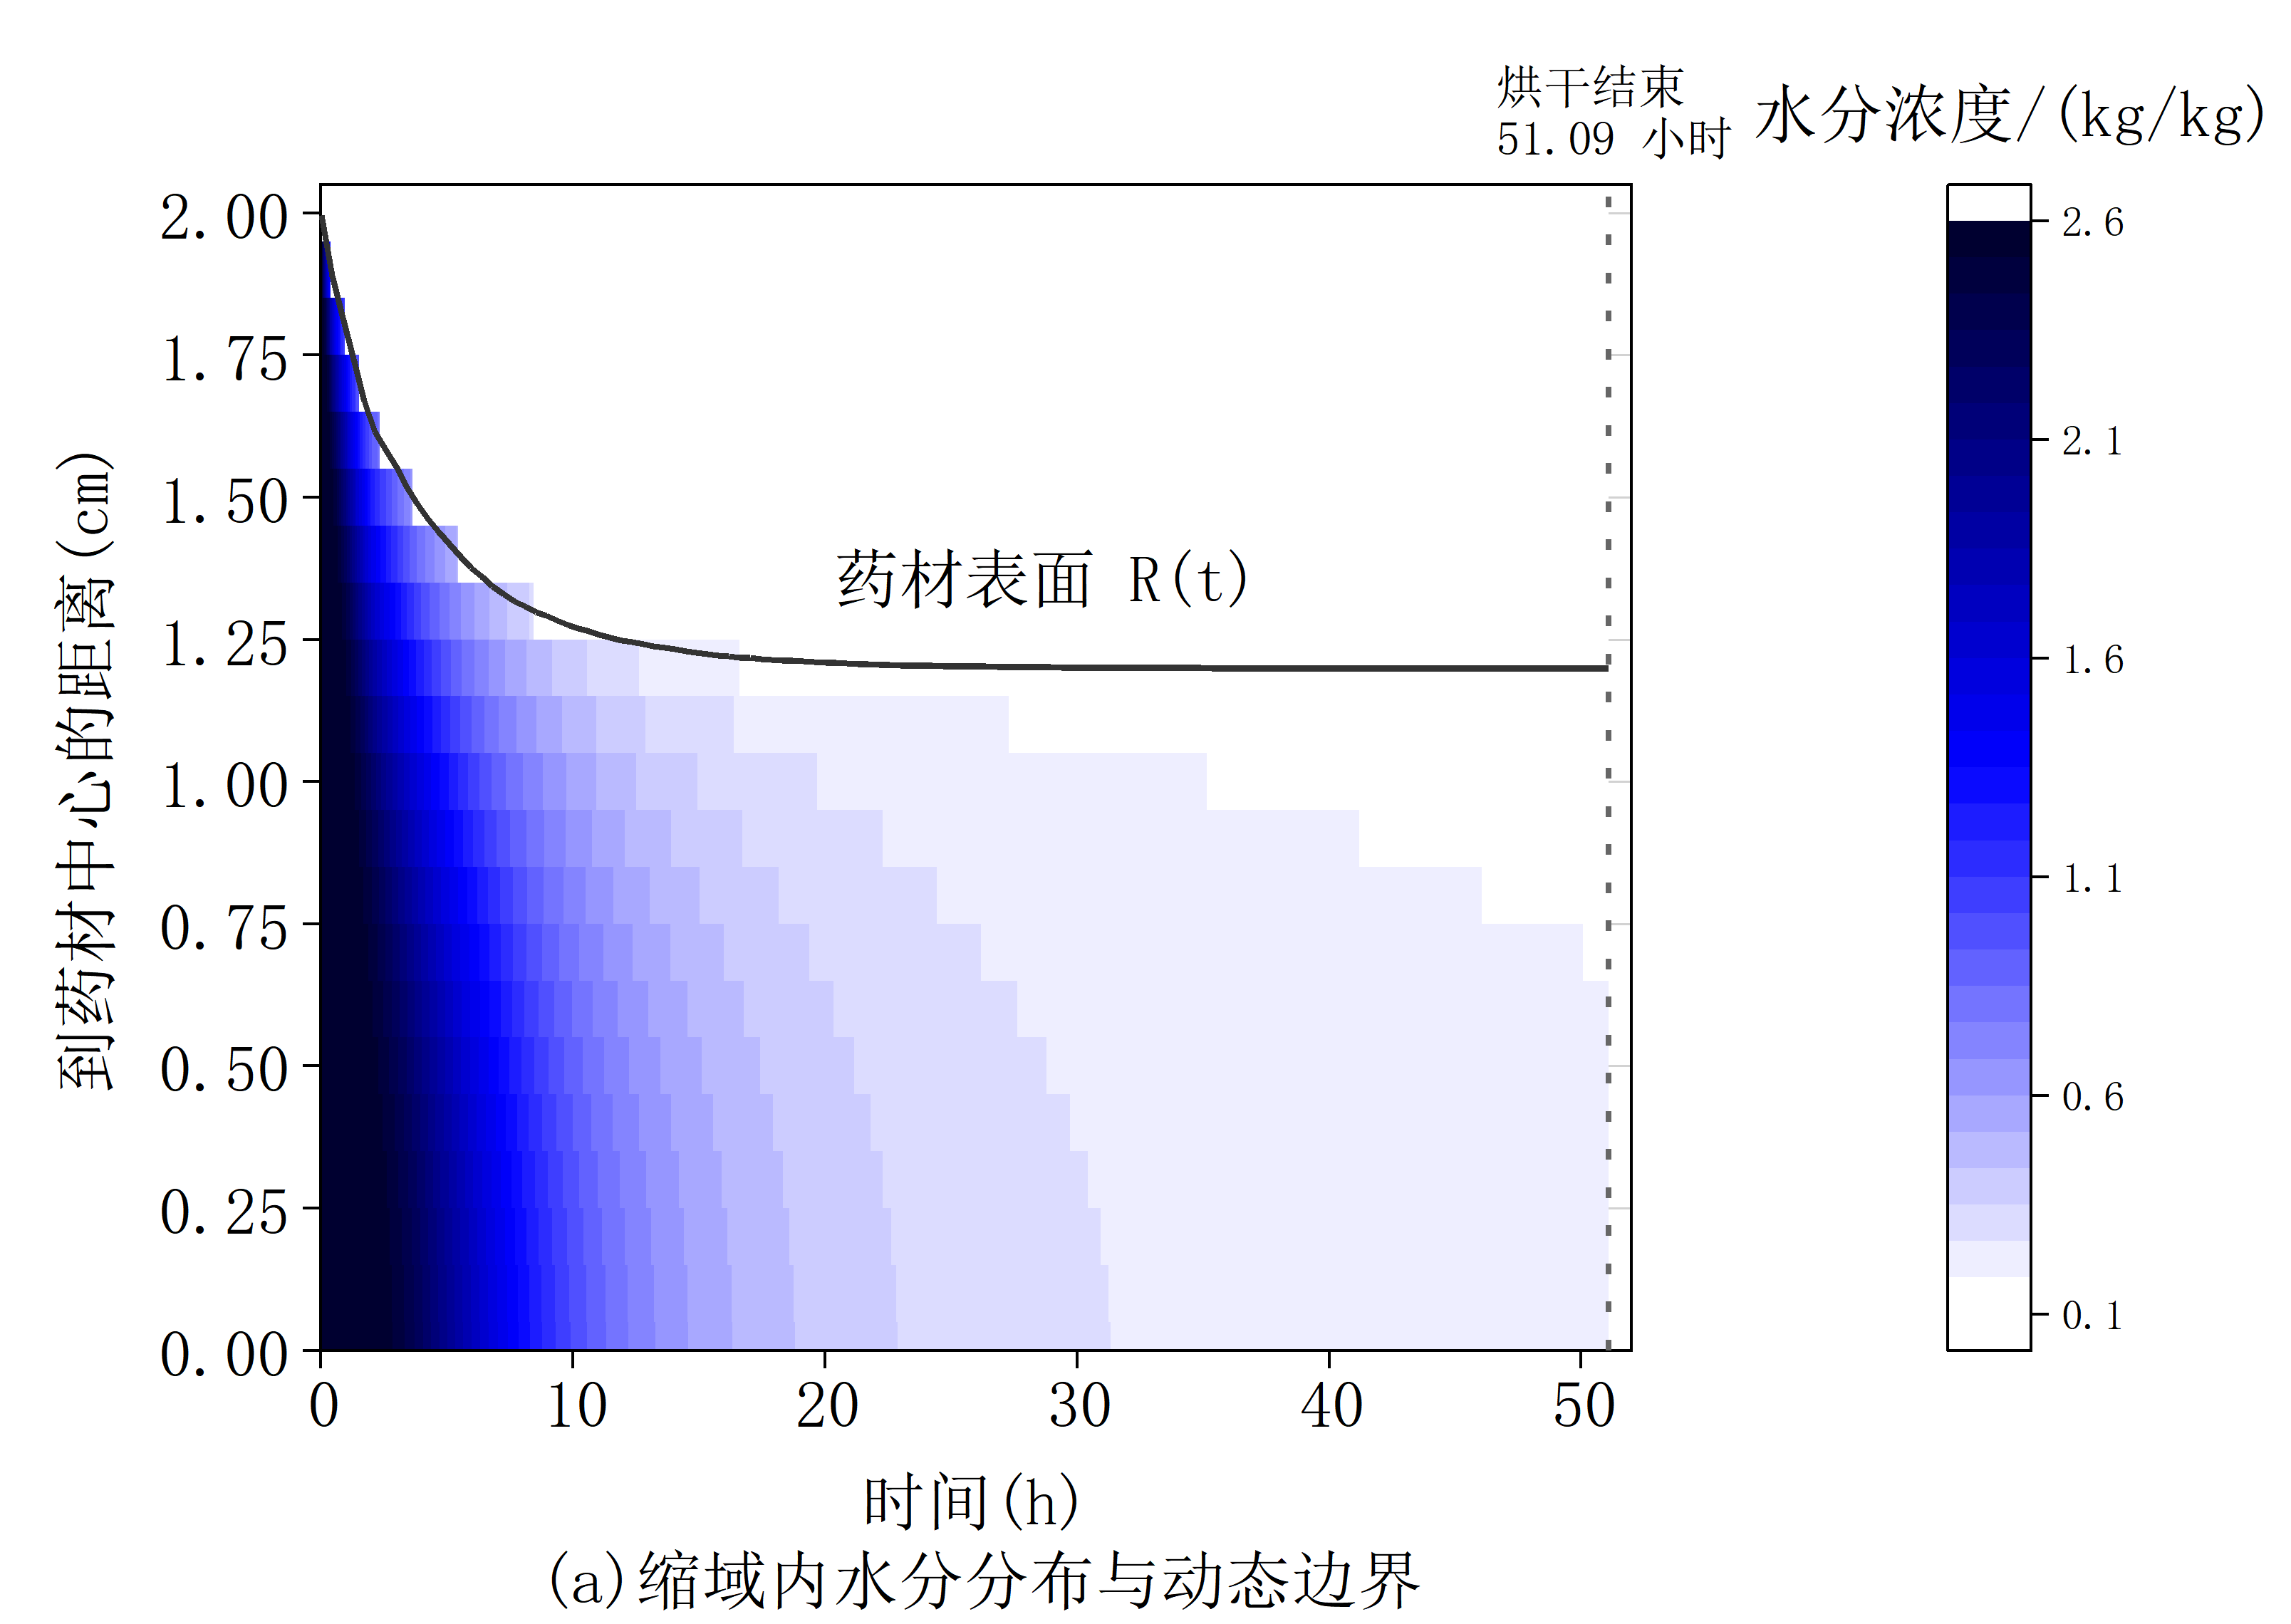
\includegraphics[trim={588.000bp 495.600bp 6.240bp 25.200bp},clip,
      height=0.022226541\unitlength]{图10(a).png}}}
  % (a)完整保留结束时间标注。
  \put(0.370318457,0.339440365){\makebox(0,0)[lb]{%
    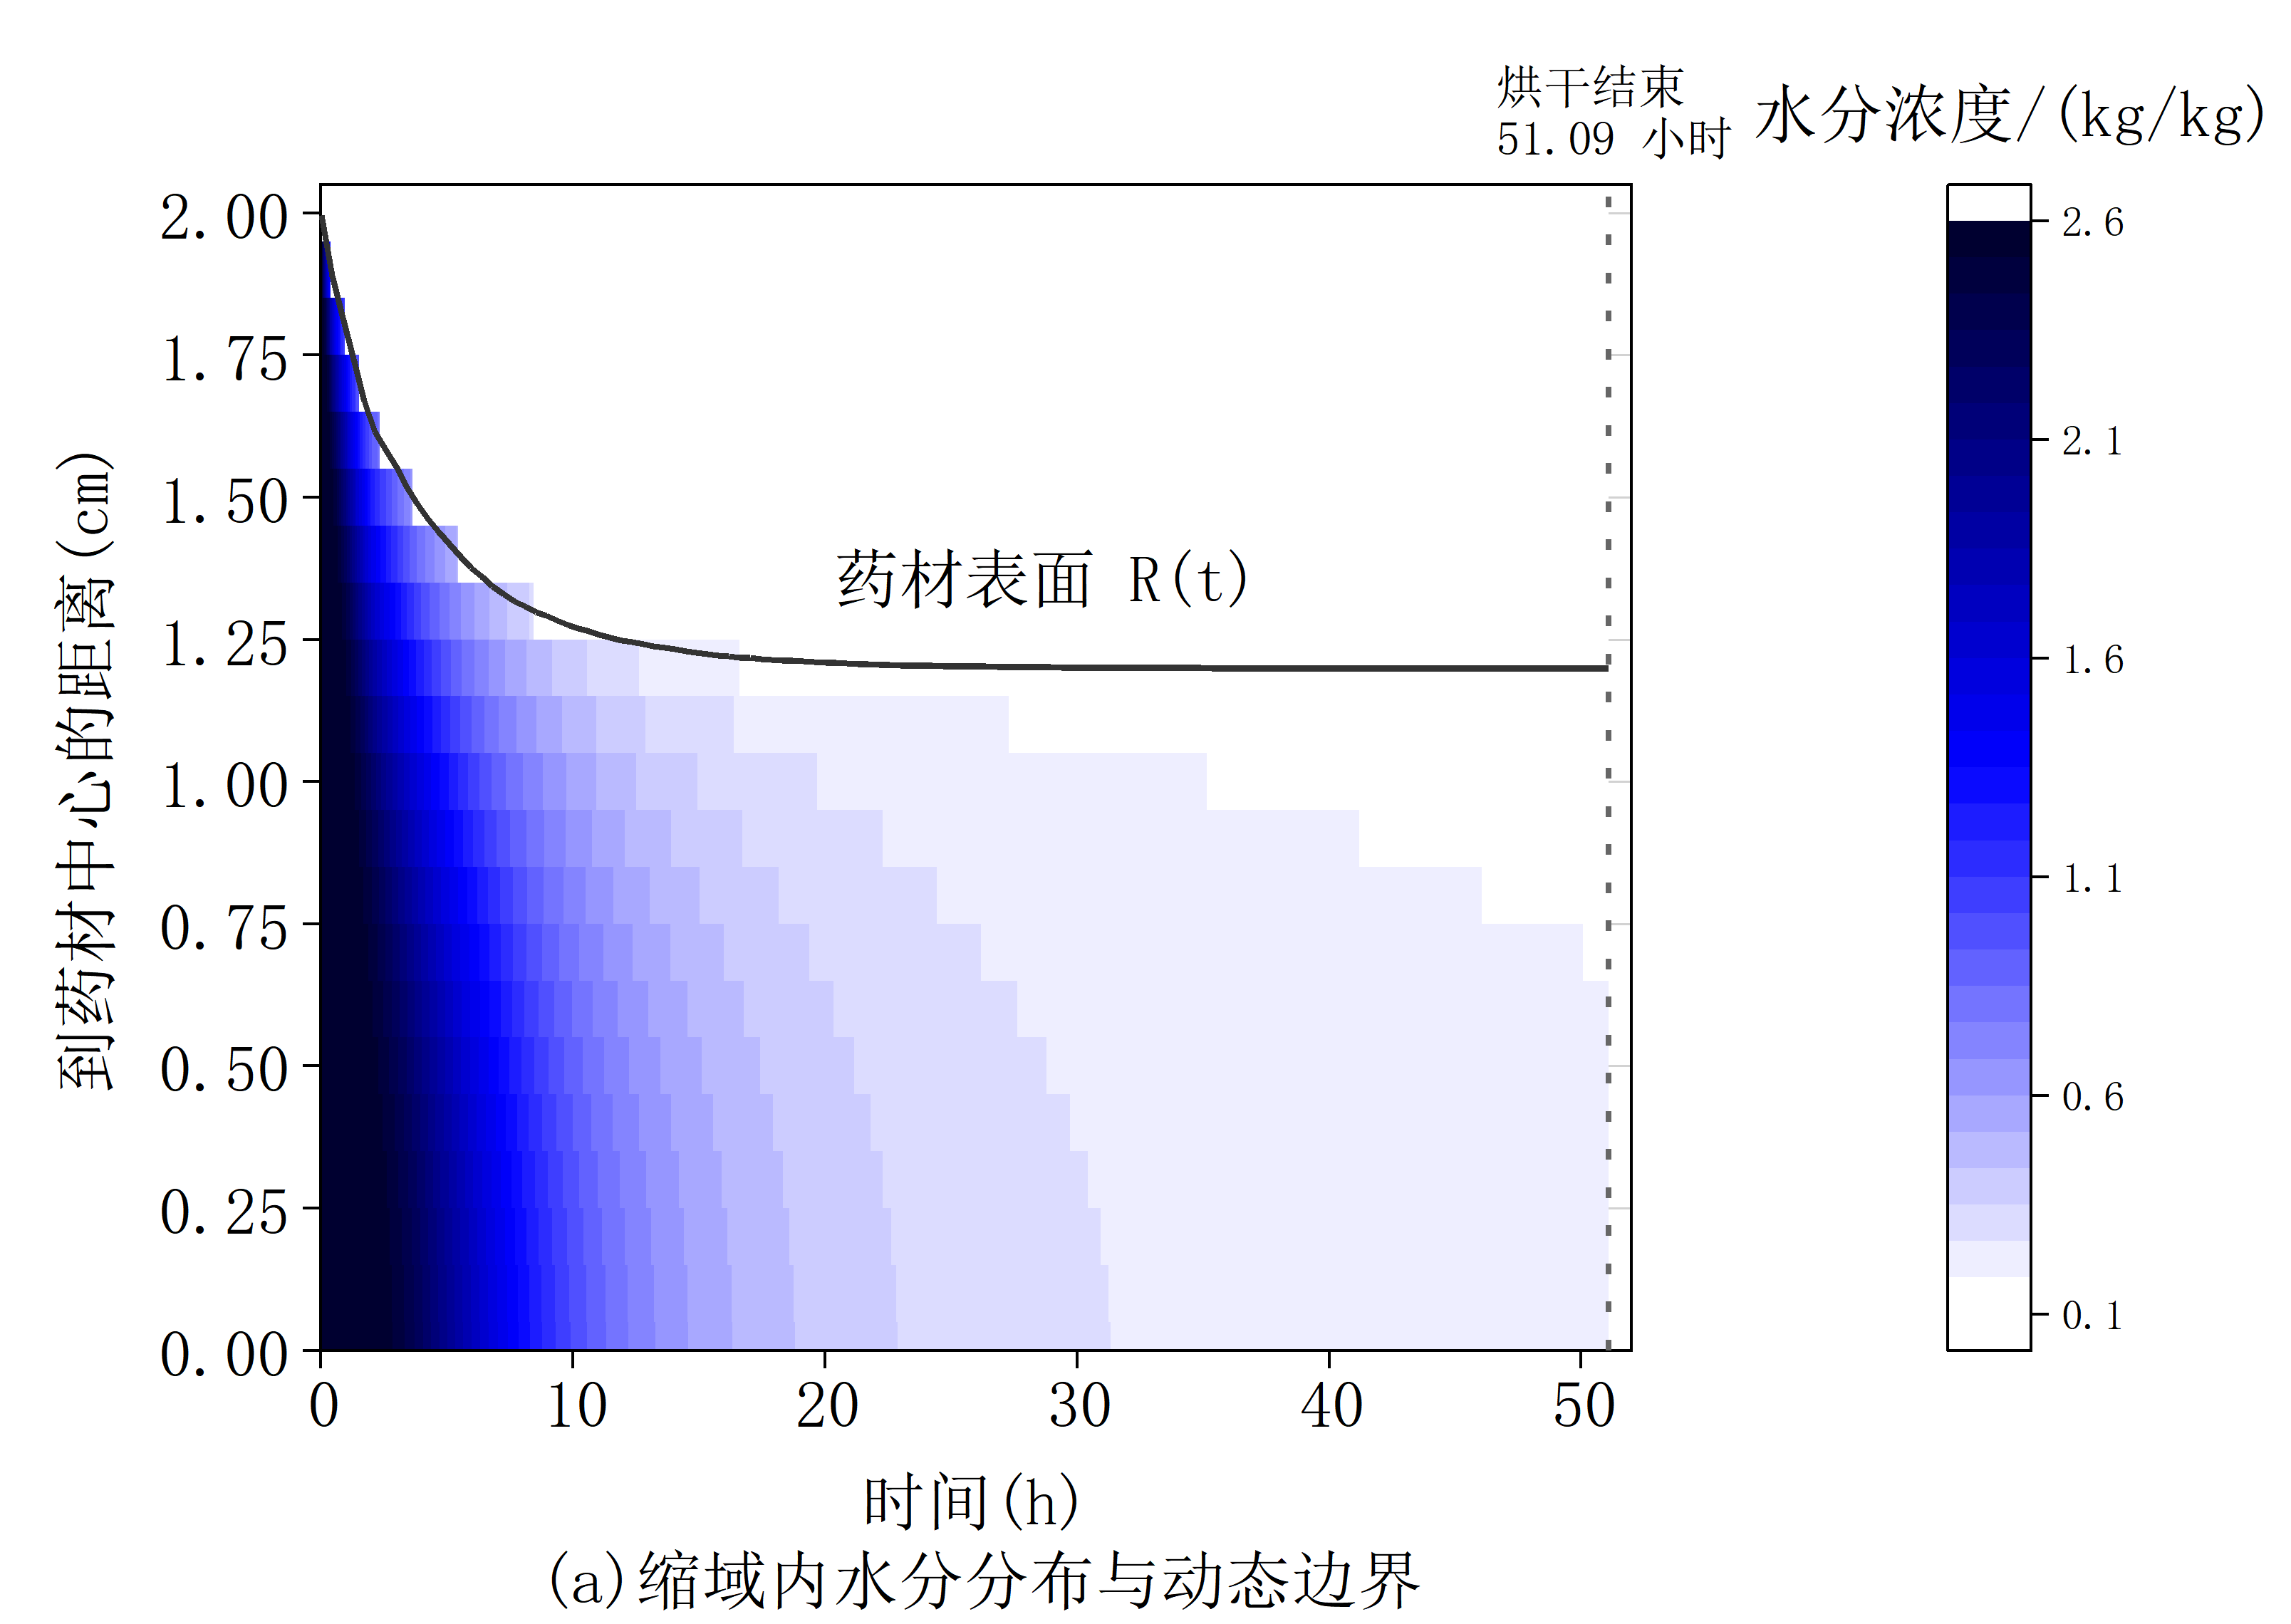
\includegraphics[trim={500.400bp 490.800bp 185.040bp 18.000bp},clip,
      height=0.032329514\unitlength]{图10(a).png}}}
  % (b)半径与平均含水率两幅原有曲线。
  \put(0.549566187,-0.000127956){\makebox(0,0)[lb]{%
    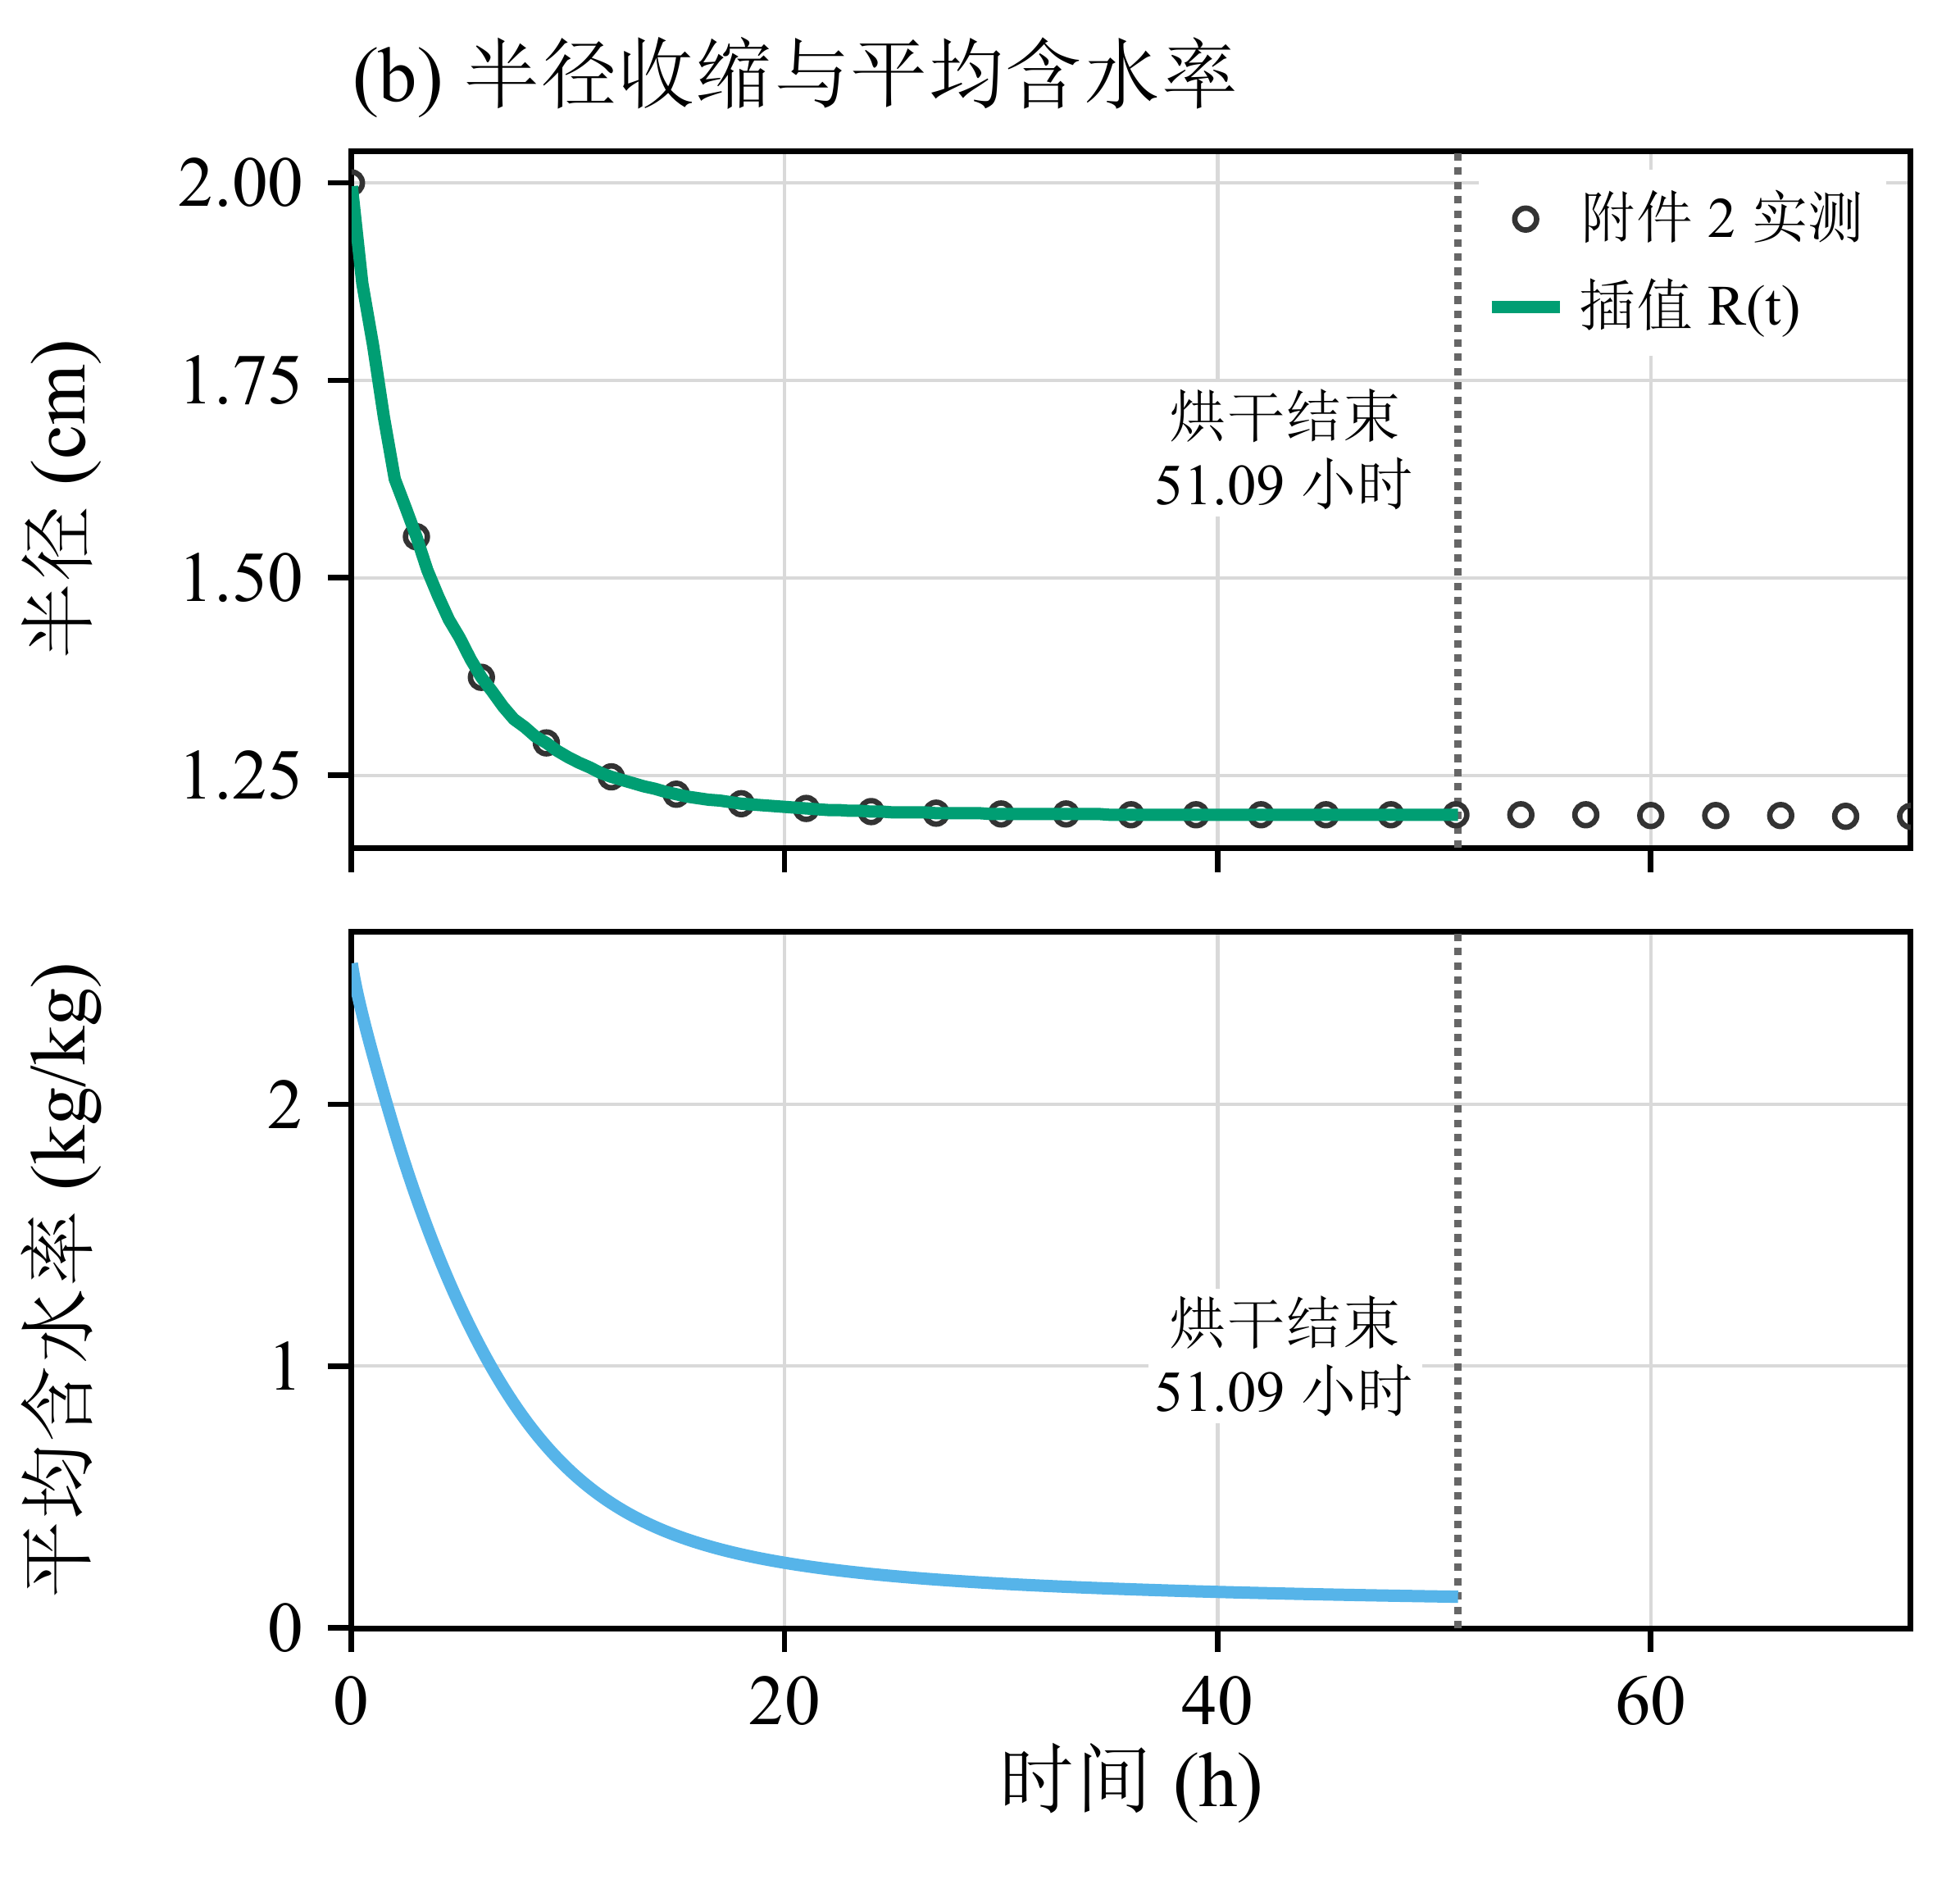
\includegraphics[width=0.450467176\unitlength]{图10(b).png}}}
\end{picture}
\caption{问题四收缩区域内的含水率分布、半径与平均含水率演化}
\label{fig:p4-drying}
\end{figure}

图\ref{fig:p4-drying}(b)中的半径曲线由附件2记录插值得到，属于模型输入；
截面平均含水率按当前截面面积加权，反映给定收缩历程下的计算响应。
半径曲线与记录点吻合不构成对含水率预测的独立验证。

$51.0905\ \mathrm{h}$的临界状态下，中心与实际表面的含水率分别为
$0.1500\cunit$和$0.0526\cunit$，仍存在内湿外干的径向差异。
结合第\ref{sec:p4-solution}节的逐节点核验，本算例仍由中心控制终点。
图\ref{fig:p4-drying}(b)中平均含水率曲线后期趋平，
说明收缩并未消除低含水率阶段的缓慢脱水特征。

\subsubsection{与固定尺寸工况的比较}

本问较问题三的$57.4721\ \mathrm{h}$缩短$6.3816\ \mathrm{h}$，约$11.10\%$。
但图\ref{fig:p34-comparison}中两问的中心含水率曲线约在$41.20\ \mathrm{h}$才交叉：
问题四前期中心含水率较高，此后才更低并率先达标。
因此，总时长较短并不意味着全过程失水更快。

\pfig{图11.pdf}{0.86}{问题三与问题四的中心含水率比较（分别采用附录3、4的物性关系）}{fig:p34-comparison}

以$D_3$、$D_4$分别表示两问的扩散系数。
由式\eqref{eq:p2-properties}、式\eqref{eq:p4-properties}，在相同含水率和温度下有
\begin{equation}
  \frac{D_4(C,T_K)}{D_3(C,T_K)}
    =0.175\exp\!\left(\frac{0.15}{C}\right).
  \label{eq:p34-diffusivity-ratio}
\end{equation}
当$C=1\cunit$和$C=0.0526\cunit$时，该比值分别约为$0.2033$和$3.03$。
附录4在较高含水率下给出的扩散能力较弱，在较低含水率下则较强，
为两问前后期表现的差异提供了物性方面的解释。

同时，问题四临界半径约为初值的$60\%$，缩短了水分迁移距离。
相关文献研究研究也表明，收缩可通过缩短迁移路径加快内部水分脱除\cite{radish-shrinkage}。
上述比较仅解释变化趋势，实际时长仍取决于全域温湿分布及表面交换，不能由局部扩散系数直接推定。
两问的热物性也同时改变，故\textbf{时长差反映尺寸收缩与物性更新的共同作用}；
若要单独量化收缩贡献，仍需在相同物性下比较固定与收缩半径两种工况。


\section{模型检验与灵敏度分析}
\label{sec:verification}
% 第九节：转录自“9.12中午_误差分析完成.docx”，统一为现有LaTeX格式。
% 原表7保留数据；原式48、原图9改由LaTeX自动编号及引用。
为评估计算结果的可靠性，分别检验数值实现、离散误差及关键参数扰动的影响。
检验沿用原计算数据，重点考察温度、含水率和临界烘干时长。

\subsection{数值检验与误差分析}
\label{sec:verification-errors}

采用独立对照与网格细化检验数值精度：
问题一温度场与Bessel--Duhamel半解析解对照；
非线性传质方程通过制造解检验\cite{mms-verification}；
各问进一步比较网格及时间步长调整后的结果。
主要指标汇总于表\ref{tab:verification}。

\begin{table}[!htbp]
  \centering
  \caption{数值检验的主要结果}
  \label{tab:verification}
  \begin{tabularx}{\textwidth}{@{}C{0.19\textwidth}YC{0.25\textwidth}@{}}
    \toprule
    检验对象 & 关键结果 & 说明\\
    \midrule
    问题一温度场
      & 最大偏差$1.68\times10^{-6}\tempunit$
      & 半解析解对照\\
    非线性传质
      & 误差$2.088\times10^{-6}\cunit$；阶约$2.00$
      & 制造解检验\\
    问题二含水率
      & 离散误差估计约$2.5\times10^{-5}\cunit$
      & 空间与时间误差之和\\
    问题四含水率
      & 最细误差估计约$1.0\times10^{-4}\cunit$
      & 固定物理位置重采样\\
    长期临界时长
      & 问题三$57.4721\ \mathrm{h}$；问题四$51.0905\ \mathrm{h}$
      & 882节点结果\\
    \bottomrule
  \end{tabularx}
\end{table}

问题一温度与含水率场均呈二阶收敛。
问题三由442细化至882节点，临界时长变化约$0.0003\ \mathrm{h}$；
问题四在882节点上将步长加倍，时长变化约$0.0001\ \mathrm{h}$，
说明达标时间对所检验的离散设置较稳定。
问题四重采样场的观测阶约为$1.63$，
故部分含水率结果的第四位小数仍有不确定性。

离散收支检验中，问题一至四的传质相对残差均不超过$1.78\times10^{-12}$，
问题一、二的热量收支相对残差均不超过$1.63\times10^{-10}$。
该检验对应本文的离散显热模型；收缩域按材料坐标的逐步收支计算。
数值场范围、严格达标条件及正文结果表与工作簿亦已核对。

现有数据缺少内部温度、径向含水率及独立烘干终点观测，
因此上述结果验证的是数值实现与离散精度，
尚不能代表相对实测值的预测误差。

\subsection{参数灵敏度分析}
\label{sec:sensitivity}

以临界烘干时长$t_*$为响应量，
对换热系数$h$、传质系数$h_m$和扩散前置系数$D_0$
分别施加$\pm10\%$的单因素扰动，其余参数保持不变。
归一化灵敏度定义为
\begin{equation}
  S_p^{\pm}
    =\frac{t_*\!\left(p(1\pm0.1)\right)-t_*(p)}
      {\pm0.1\,t_*(p)},
  \qquad p\in\{h,h_m,D_0\}.
  \label{eq:parameter-sensitivity}
\end{equation}

两问各计算1组基准和6组扰动工况，均采用222节点及原时间步长。
基准时长分别为$57.4706\ \mathrm{h}$和$51.0906\ \mathrm{h}$，
与882节点结果相差小于$0.002\ \mathrm{h}$。
$D_0$扰动仅改变前置系数；
问题四保持给定半径历程$R(t)$不变。
各参数引起的时长相对变化见图\ref{fig:parameter-sensitivity}。

\pfig{图12.png}{0.98}{参数增减10\%时临界烘干时长的相对变化}{fig:parameter-sensitivity}

两问均表现为扩散前置系数影响最大、传质系数次之、换热系数最小。
$D_0$增加$10\%$时，烘干时长减少约$8\%$；
降低$10\%$时，时长增加约$9.8\%$。
传质系数引起的时长变化约为$1.0\%$--$1.3\%$（问题三）
和$0.4\%$--$0.6\%$（问题四），
换热系数仅约$0.01\%$--$0.02\%$。

扩散参数扰动的影响远大于网格细化误差，
说明后续提高预测精度应优先标定扩散参数，
尤其是低含水率阶段的扩散能力。
该结论限于题给工况及给定收缩历程，
不能直接用于确定最优温度或风速。


% 第十节接续前文，避免浮动屏障触发节首换页。
\let\savedSectionFloatBarrier\FloatBarrier
\let\FloatBarrier\relax
\section{模型评价与改进方向}
\let\FloatBarrier\savedSectionFloatBarrier
\label{sec:evaluation}
% 第十节：转录自“9.12中午_误差分析完成.docx”，优缺点分别采用“1、2、……”编号。
\subsection{模型优点}

\begin{enumerate}[label=\arabic*、,leftmargin=2em,labelsep=0pt,itemsep=0.5em,topsep=0.3em]
\item \textbf{模型具有较强的物理解释性。}
本文从药材内部热质传递机理出发，
逐步建立径向热质传递模型、变物性热质耦合模型以及收缩动边界模型，
能够较全面地描述烘干过程中温度、水分及尺寸变化规律。

\item \textbf{模型具有较好的递进性。}
针对不同阶段的研究需求，逐步引入物性变化、烘干判据和尺寸收缩因素，
在保证计算可行性的同时提高了模型与实际干燥过程的符合程度。

\item \textbf{数值求解过程稳定可靠。}
采用表面加密有限体积法和中点物性迭代处理模型计算，
并通过多种检验方法验证结果的稳定性，提高了模型预测精度。
\end{enumerate}

\subsection{模型缺点}

\begin{enumerate}[label=\arabic*、,leftmargin=2em,labelsep=0pt,itemsep=0.5em,topsep=0.3em]
\item \textbf{部分复杂物理过程进行了简化。}
模型中忽略了蒸发潜热、辐射换热等因素，
并采用一维径向假设描述药材内部传递过程，
对实际复杂结构药材的适用性存在一定限制。

\item \textbf{部分参数依赖题目给定或等效处理。}
水分扩散系数、换热系数等参数仍需要更精确的实验数据支持，
进一步完善参数测定可提高模型预测能力。
\end{enumerate}

